% !TEX program = xelatex
\documentclass[12pt, a4paper, UTF8]{ctexart}

\usepackage[margin=2.5cm]{geometry}
\usepackage{amsmath, amssymb}
\usepackage{bm}
\usepackage{graphicx}
\usepackage{booktabs}
\usepackage{longtable}
\usepackage{float}
\usepackage{xcolor}
\usepackage{listings}
\usepackage{caption}
\usepackage{enumitem}
\usepackage[section]{placeins}
\usepackage[colorlinks=true, linkcolor=black, urlcolor=blue, citecolor=black]{hyperref}

\graphicspath{{results/plots/}}

% 浮动体排版优化：允许图片浮动回填文字空隙，消除页尾大片留白
\renewcommand{\topfraction}{0.92}
\renewcommand{\bottomfraction}{0.55}
\renewcommand{\textfraction}{0.06}
\renewcommand{\floatpagefraction}{0.85}
\setcounter{topnumber}{3}
\setcounter{totalnumber}{5}
\raggedbottom
\captionsetup{font=small, labelfont=bf, skip=5pt}

% 代码排版样式
\definecolor{codegray}{RGB}{245,245,245}
\definecolor{codegreen}{RGB}{0,128,0}
\definecolor{codeblue}{RGB}{0,0,200}
\lstset{
  language=Python,
  basicstyle=\ttfamily\scriptsize,
  keywordstyle=\color{codeblue}\bfseries,
  commentstyle=\color{codegreen}\itshape,
  stringstyle=\color{teal},
  backgroundcolor=\color{codegray},
  numbers=left,
  numberstyle=\tiny\color{gray},
  numbersep=8pt,
  frame=single,
  breaklines=true,
  tabsize=4,
  showstringspaces=false,
  columns=flexible,
  extendedchars=false
}

\title{\textbf{多变换域联合的信号调制特征识别与\\滤波优化系统}\\[0.5em]
\large 数字信号处理综合大作业实践报告（题目三：创新拓展型）}
\author{李宸威 \quad 学号：202464820504 \\[0.4em]
班级：24级超级机器人珠峰班 \quad 指导教师：俞祝良}
\date{\today}

\begin{document}

\maketitle

\begin{abstract}
本报告围绕数字调制通信信号的处理需求，设计并实现了一个多变换域联合的信号调制特征识别与滤波优化系统。系统以 Python 为实现平台，完整覆盖离散信号建模、时域卷积、DTFT/DFT/Z 变换多域联合分析、FIR/IIR 滤波器设计与迭代优化、NLMS 自适应滤波、调制方式自动识别与解调级误码率评估等环节。针对 ASK/FSK/PSK 三种数字调制信号，系统在 10\,dB 信噪比下实现了 100\% 的自动识别准确率；滤波器参数三维网格扫描（阶数$\times$窗函数$\times$截止频率）使信噪比改善最高达 9.60\,dB；消融实验定量证明多域联合识别相比最佳单一域取得 +31.1\% 的准确率增益。报告详细阐述各环节的理论依据、实现方法与实验结果，关键程序代码见附录。
\end{abstract}

\tableofcontents
\newpage

%==============================================================
\section{引言}
%==============================================================

\subsection{选题背景}

在现代数字通信系统中，信号经信道传输后不可避免地叠加噪声，接收端需要完成两个核心任务：一是通过滤波尽可能恢复纯净信号，二是自动识别信号的调制方式以便正确解调。单一域（仅时域或仅频域）的分析手段往往只能刻画信号的局部特征，难以应对调制方式间的相似性（如 ASK 与 PSK 的频谱均为单峰结构）。本题要求建立``时域--频域--Z域''三维联合分析思维，完成调制信号的特征分析、噪声抑制与自动识别，并对滤波器性能进行迭代优化。

\subsection{总体设计}

系统采用模块化流水线结构，共 11 个处理步骤，全部由 Python（NumPy、SciPy、Matplotlib）实现。整体流程与模块对应关系如表~\ref{tab:pipeline} 所示。

\begin{table}[H]
\centering
\caption{系统处理流水线与模块对应关系}
\label{tab:pipeline}
\resizebox{\textwidth}{!}{%
\begin{tabular}{cllc}
\toprule
步骤 & 内容 & 核心模块/函数 & 输出 \\
\midrule
1 & 调制信号建模与生成 & \texttt{generator} & 纯净/含噪信号 \\
2 & 时域分析与卷积平滑 & \texttt{analyzer} & 图 01--02 \\
3 & DTFT/DFT/Z 域多域分析 & \texttt{analyzer} & 图 03--05、13、15 \\
4 & FIR/IIR 滤波器设计 & \texttt{filter\_design} & 图 06--07、系统函数 \\
5 & 滤波器参数迭代优化 & \texttt{filter\_design.iterative\_optimize} & 图 09、09b \\
6 & NLMS 自适应滤波 & \texttt{filter\_design.lms\_filter} & 图 10、10b \\
7 & 调制方式自动识别 & \texttt{recognizer.classify\_signal} & 图 11 \\
8 & 性能评估（SNR/BER/复杂度） & \texttt{recognizer} & 图 12 \\
9 & SNR 扫描蒙特卡洛实验 & \texttt{recognizer.run\_snr\_sweep} & 图 14 \\
10 & 单域 vs 多域消融实验 & \texttt{recognizer.run\_domain\_ablation} & 图 16 \\
11 & 评估报告生成 & \texttt{recognizer.generate\_report} & logs.txt \\
\bottomrule
\end{tabular}%
}
\end{table}

实验参数统一在 \texttt{config.py} 中管理：采样率 $F_s=10\,\mathrm{kHz}$，符号速率 10\,Baud（每符号 1000 点），信息长度 20 bit，默认信噪比 SNR $=10$\,dB，随机种子 42 保证结果可复现。三种调制的载波参数为：ASK 载频 $f_c=1\,\mathrm{kHz}$（OOK，$A_1{=}1, A_0{=}0$）；FSK 两个符号频率 $f_1=800\,\mathrm{Hz}$、$f_2=1200\,\mathrm{Hz}$；PSK（BPSK）载频 $1\,\mathrm{kHz}$、相位 $\{0,\pi\}$。由于符号频率均为符号率整数倍，逐符号生成的 FSK 相位天然连续（等效 CPFSK），频谱双峰结构干净。

\subsection{主要工作与工作量}

本作业围绕题目五项实施要点完成的主要工作如下：

\begin{enumerate}
  \item \textbf{系统搭建}：自主设计并实现覆盖``建模--分析--滤波--识别--评估''全链路的 DSP 仿真系统，含 7 个源模块、约 3660 行 Python 代码，单命令复现全部实验，自动产出 29 张结果图与 1 份六章节量化评估报告；
  \item \textbf{信号建模}：实现 ASK/FSK/PSK 三种数字调制信号模型与 AWGN 信道（式(1)--(4)），比特序列与噪声流分离管理，支持可控复现；
  \item \textbf{多域分析}：实现时域卷积平滑与统计特征、DFT/DTFT 频谱分析、基于 AR 参数模型的 Z 域零极点估计，并完成三种变换应用差异的对比分析（图~\ref{fig:cmp15}）；
  \item \textbf{滤波优化}：设计 FIR/IIR 带通滤波器并完成``阶数$\times$窗函数$\times$截止频率''三维网格（84 种组合/调制）迭代优化，以保真度与归一化 $\Delta$SNR 加权评分自动选型；
  \item \textbf{自适应滤波}：实现标准 LMS 与 NLMS 两种算法，完成步长扫描、收敛性分析、权值演化追踪与按条件择优策略；
  \item \textbf{解调评估}：构建三种调制的完整解调链路（包络检波/相关/相干解调），建立解调级误码率（BER）评估体系，并量化各方法的运算复杂度；
  \item \textbf{系统实验}：完成 7 个 SNR 点$\times$5 次蒙特卡洛的性能扫描实验，以及``仅时域/仅频域/仅Z域/多域联合''四模式消融实验，定量回答``多域联合优势''问题；
  \item \textbf{问题排查}：针对开发中发现的 4 个典型问题完成根因分析与修复验证（详见 \S\ref{sec:debug}）。
\end{enumerate}

本系统完整源代码、实验结果图表与评估报告已开源于 GitHub 仓库：\url{https://github.com/lcw578/-}。

%==============================================================
\section{基本理论}
%==============================================================

\subsection{数字调制信号模型}

设二进制比特序列 $b_m \in \{0,1\}$，$m=0,1,\dots,M-1$，每符号采样点数 $N_s = F_s T_s = 1000$。

\textbf{（1）ASK（幅移键控，OOK）}：用幅度携带信息，
\begin{equation}
s_{\mathrm{ASK}}(n) = A(b_m)\cos(2\pi f_c n T_s), \quad A(b_m)=\begin{cases}A_1=1, & b_m=1\\ A_0=0, & b_m=0\end{cases}
\end{equation}

\textbf{（2）FSK（频移键控）}：用频率携带信息，
\begin{equation}
s_{\mathrm{FSK}}(n) = \cos\!\left(2\pi f_{b_m} n T_s\right), \quad f_{b_m}=\begin{cases}f_1=800\,\mathrm{Hz}, & b_m=0\\ f_2=1200\,\mathrm{Hz}, & b_m=1\end{cases}
\end{equation}

\textbf{（3）PSK（相移键控，BPSK）}：用相位携带信息，
\begin{equation}
s_{\mathrm{PSK}}(n) = \cos\!\left(2\pi f_c n T_s + \varphi_{b_m}\right), \quad \varphi_{b_m}=\begin{cases}0, & b_m=0\\ \pi, & b_m=1\end{cases}
\end{equation}

\textbf{信道噪声模型（AWGN）}：叠加加性高斯白噪声
\begin{equation}
x(n) = s(n) + v(n), \quad v(n)\sim\mathcal{N}(0,\sigma_v^2), \quad \sigma_v^2 = \frac{P_s}{10^{\mathrm{SNR}/10}}
\end{equation}
其中 $P_s=\frac{1}{N}\sum_n s^2(n)$ 为信号功率。SNR $=10$\,dB 时 $\sigma_v^2 = P_s/10$。

\subsection{时域分析与卷积平滑}

卷积是 LTI 系统分析的基础运算。时域平滑采用矩形核均值滤波器：
\begin{equation}
h[k] = \frac{1}{L},\ k=0,1,\dots,L-1, \qquad y[n] = \sum_{k} x[k]\,h[n-k] = \frac{1}{L}\sum_{k=n-L+1}^{n} x[k]
\end{equation}
窗长 $L$ 越大平滑（去噪）能力越强，但会模糊信号边缘细节，实验中对 $L\in\{5,11,21,51\}$ 进行对比。

信号包络由 Hilbert 变换构造解析信号获得：
\begin{equation}
\tilde{x}(n) = x(n) + \mathrm{j}\,\hat{x}(n), \qquad \mathrm{env}(n) = |\tilde{x}(n)|
\end{equation}
其中 $\hat{x}$ 为 Hilbert 变换。包络的变异系数 $\mathrm{CV}=\sigma_{\mathrm{env}}/\mu_{\mathrm{env}}$ 是区分幅度键控与恒包络调制的关键时域特征。

\subsection{DTFT 与 DFT 及其关系}

\textbf{DTFT（离散时间傅里叶变换）}是连续谱：
\begin{equation}
X(e^{\mathrm{j}\omega}) = \sum_{n=-\infty}^{\infty} x[n]\,e^{-\mathrm{j}\omega n}, \qquad \omega \in [-\pi, \pi)
\end{equation}

\textbf{DFT（离散傅里叶变换）}是有限长序列的离散谱：
\begin{equation}
X[k] = \sum_{n=0}^{N-1} x[n]\,e^{-\mathrm{j}2\pi kn/N}, \quad k=0,1,\dots,N-1
\end{equation}

二者的核心关系为：\textbf{DFT 是 DTFT 在 $\omega_k = 2\pi k/N$ 处的等间隔采样}，频率分辨率 $\Delta f = F_s/N$。本系统 $N=20000$，$\Delta f = 0.5\,\mathrm{Hz}$。工程实现中，DTFT 通过零填充 FFT 在密集频点上逼近；DFT 直接由 FFT 计算。DFT 谱线支撑峰值检测（调制识别的频域核心特征），DTFT 连续谱形则直观呈现带宽与旁瓣结构。

\subsection{Z 变换与零极点分析}

序列的 Z 变换定义为 $X(z)=\sum_n x[n]z^{-n}$。对 LTI 系统，传递函数 $H(z)=B(z)/A(z)$ 的零极点分布完全刻画其频率选择性：极点在单位圆内靠近单位圆处对应谐振峰，极点角位置 $\theta$ 映射模拟频率 $f \approx \theta F_s/(2\pi)$。

离散信号本身不具有有理形式的 Z 变换，本系统采用\textbf{AR 参数模型}对信号进行 Z 域建模：
\begin{equation}
x(n) = \sum_{k=1}^{p} a_k\, x(n-k) + e(n) \quad\Longleftrightarrow\quad H_{\mathrm{AR}}(z) = \frac{1}{1-\sum_{k=1}^{p} a_k z^{-k}}
\end{equation}
AR 系数 $a_k$ 由 Yule--Walker 方程 $R\,\bm{a}=\bm{r}$ 求解（自相关矩阵 $R$ 为 Toeplitz 结构，用 Levinson--Durbin 递推高效求解），随后对 $A(z)$ 求根得到极点。主极点模长 $r=|p_{\max}|$ 反映谱线锐度（品质因数）：恒包络调制（FSK/PSK）的载波谱线极尖锐，$r\to 1$；而 ASK 因通断键控使谱线展宽，$r$ 明显下降——这是 Z 域区分幅度键控与恒包络调制的物理依据。

\subsection{FIR/IIR 滤波器设计}

\textbf{FIR 窗函数法}：以理想带通响应 $h_d[n]$ 与窗函数 $w[n]$ 相乘截断：
\begin{equation}
h_d[n] = \frac{\sin\big(\omega_2(n-\alpha)\big)-\sin\big(\omega_1(n-\alpha)\big)}{\pi (n-\alpha)}, \qquad h[n] = h_d[n]\,w[n]
\end{equation}
其中 $\alpha=N/2$ 保证线性相位。本系统对比 Hamming、Hann、Blackman、Kaiser 四种窗。

\textbf{IIR 滤波器}：基于模拟原型经双线性变换 $s \leftarrow \frac{2}{T}\frac{1-z^{-1}}{1+z^{-1}}$ 设计。Butterworth 幅度平方函数为
\begin{equation}
|H(\mathrm{j}\Omega)|^2 = \frac{1}{1+(\Omega/\Omega_c)^{2N}}
\end{equation}
另对比 Chebyshev I 型（通带等纹波）与椭圆滤波器（双带等纹波、过渡带最窄）。

\textbf{零相位滤波}：使用 filtfilt（前向+后向滤波），等效频率响应为 $|H_{\mathrm{eff}}(e^{\mathrm{j}\omega})|=|H(e^{\mathrm{j}\omega})|^2$，相位严格为零，完全消除群延迟引起的波形失真，代价是乘加次数加倍。

\subsection{LMS 与 NLMS 自适应滤波}

自适应噪声对消（ANC）结构：参考信道输入与噪声相关的信号 $x(n)$，期望响应 $d(n)=s(n)+v(n)$，自适应滤波器输出噪声估计 $\hat{v}(n)=\sum_k w_k x(n-k)$，误差
\begin{equation}
e(n) = d(n) - \hat{v}(n) = s(n) + \big(v(n)-\hat{v}(n)\big)
\end{equation}
当权向量收敛到维纳解时 $v(n)-\hat{v}(n)\to 0$，误差即为去噪信号。

\textbf{LMS 算法}按最速下降方向更新权值：
\begin{equation}
\bm{w}(n+1) = \bm{w}(n) + 2\mu\, e(n)\,\bm{x}(n)
\end{equation}
收敛条件为 $0<\mu<1/(M P_x)$（$M$ 为滤波器阶数，$P_x$ 为输入功率）。标准 LMS 步长与输入功率强耦合：白噪声输入下权值需收敛到类冲激响应，收敛时间常数约为 $M/(2\mu)$ 量级，短记录内常来不及收敛。

\textbf{NLMS（归一化 LMS）}对更新步长按输入向量能量归一化：
\begin{equation}
\bm{w}(n+1) = \bm{w}(n) + \frac{\mu\, e(n)\,\bm{x}(n)}{\bm{x}^{\mathrm{T}}(n)\bm{x}(n)+\delta}, \qquad \mu\in(0,2)
\end{equation}
步长与输入功率无关，收敛速度大幅提升且对输入电平变化鲁棒。代价是稳态失调随 $\mu$ 增大而增大，存在``收敛速度--稳态精度''折中，实验通过步长扫描定量刻画。

\subsection{解调与误码率（BER）}

波形级指标（SNR、相关系数）之外，系统进一步实现解调级评估：
\begin{itemize}
  \item \textbf{ASK 包络检波}：Hilbert 包络按符号积累能量 $E_m$，与自适应门限比较判决；
  \item \textbf{FSK 相关解调}：每符号分别与两个本地载波作相关运算 $\left|\sum_n s(n)\cos(2\pi f_i nT_s)\right|$，择大判决；
  \item \textbf{PSK 相干解调}：每符号与本地同相载波相关，按极性判决。
\end{itemize}
误码率定义为 $\mathrm{BER} = N_{\mathrm{err}}/N_{\mathrm{bits}}$，直接反映滤波对通信正确性的改善。

\subsection{调制识别特征体系}

多域联合识别使用三类特征（表~\ref{tab:features}）。

\begin{table}[H]
\centering
\caption{调制识别特征体系}
\label{tab:features}
\resizebox{\textwidth}{!}{%
\begin{tabular}{clll}
\toprule
特征域 & 特征 & 定义 & 判别意义 \\
\midrule
时域 & 包络变异系数 CV & $\sigma_{\mathrm{env}}/\mu_{\mathrm{env}}$ & ASK 大（$>0.5$），恒包络小（$<0.3$） \\
时域 & 相位跳变率 & $P(|\Delta\phi|>\pi/2)$ & PSK 符号边界相位反转 \\
时域 & 瞬时频率标准差 & $\sigma_{f_i}$ & FSK 双频切换使 $\sigma_{f_i}$ 大 \\
频域 & 显著谱峰数量 & 峰值检测（阈值 0.3） & FSK 双峰，ASK/PSK 单峰 \\
频域 & 谱集中度 & 主峰 $\pm 100$\,Hz 能量占比 & 单载波调制能量集中 \\
Z 域 & 主极点半径 $r$ & AR 模型 $|p_{\max}|$ & 恒包络 $r\ge 0.96$，ASK 谱线展宽 \\
\bottomrule
\end{tabular}%
}
\end{table}

分类器采用加权投票规则：每条规则命中时为对应类别累加分数，最终取得分最高者为识别结果，置信度为该类得分占总分比例。

%==============================================================
\section{系统实现}
%==============================================================

\subsection{开发环境与工程结构}

开发与实验环境如表~\ref{tab:env} 所示，工程按``参数--生成--分析--滤波--解调--识别''职责划分为 7 个模块（合计约 3660 行），主流程入口为 \texttt{main.py}，单命令即可复现全部实验与图表。

\begin{table}[H]
\centering
\caption{开发环境}
\label{tab:env}
\begin{tabular}{ll}
\toprule
项目 & 配置 \\
\midrule
操作系统 & Windows x64 \\
编程语言 & Python 3.11.15 \\
数值计算 & NumPy 2.4.6、SciPy 1.17.1 \\
可视化 & Matplotlib 3.9.2（Agg 后端，SimHei 中文字体） \\
报告排版 & \LaTeX（XeLaTeX + ctex，MiKTeX 25.12） \\
版本管理 & Git（GitHub 仓库 \url{https://github.com/lcw578/-}） \\
\bottomrule
\end{tabular}
\end{table}

\begin{table}[H]
\centering
\caption{工程模块划分}
\label{tab:modules}
\begin{tabular}{lll}
\toprule
模块 & 行数 & 职责 \\
\midrule
\texttt{config.py} & 112 & 全局参数中心（采样/载波/滤波器/自适应/SNR 扫描） \\
\texttt{utils/generator.py} & 260 & 比特序列、ASK/FSK/PSK 调制、AWGN 信道 \\
\texttt{utils/analyzer.py} & 701 & 卷积平滑、DFT/DTFT/Z 域分析、多域可视化 \\
\texttt{utils/filter\_design.py} & 857 & FIR/IIR 设计、迭代优化、LMS/NLMS 自适应滤波 \\
\texttt{utils/demodulator.py} & 175 & 三种调制解调与 BER 计算 \\
\texttt{utils/recognizer.py} & 1036 & 特征提取、分类识别、性能评估、扫描/消融实验 \\
\texttt{main.py} & 516 & 11 步主流程调度 \\
\bottomrule
\end{tabular}
\end{table}

\subsection{各模块关键实现细节}

\textbf{（1）信号生成与信道建模。}三种调制波形按符号分段生成；由于各载频均为符号率（10\,Hz）的整数倍，符号边界处载波相位差为零，逐符号独立生成即等效连续相位调制。比特序列由独立种子 \texttt{RandomState(42)} 驱动，而 AWGN 使用全局随机流——二者分离使不同试验间比特保持一致、噪声实现相互独立，便于蒙特卡洛统计。

\textbf{（2）多域分析。}DFT 单边谱归一化时对 DC 与 Nyquist 分量不作加倍处理，避免端点幅度失真；DTFT 通过 4096/8192 点零填充 FFT 在密集频点逼近；AR 建模取信号\textbf{中段} 4000 点（覆盖 4 个符号），保证 FSK 的两个载频成分都进入自相关估计，模型阶数取 6——阶数过高（如 12）会对带通噪声过拟合，产生大量虚假谐振极点，反而破坏特征区分度（排查过程见 \S\ref{sec:debug} 问题 3）。

\textbf{（3）滤波器设计与优化。}\texttt{firwin(numtaps=order+1)} 使参数``阶数''与教科书定义严格一致；\texttt{filtfilt} 零相位滤波对短信号保护 \texttt{padlen} 并自动回退 \texttt{lfilter}。迭代优化的综合评分设计为
\begin{equation}
\mathrm{Score} = 0.6\times\mathrm{corr} + 0.4\times\frac{\min(\max(\Delta\mathrm{SNR},0),15)}{15}
\end{equation}
将 SNR 改善以 15\,dB 为参考上限归一化到 $[0,1]$，与保真度等权融合，避免原始评分公式中 $ \mathrm{SNR}/50 $ 归一化基准无依据的问题。

\textbf{（4）NLMS 自适应滤波。}ANC 参考信道取含当前时刻样本的噪声序列，此时互相关向量 $p[0]=\sigma_v^2>0$，维纳解为类冲激响应 $\bm{w}^\ast=[1,0,\dots,0]^\ast$（该设计的关键性见 \S\ref{sec:debug} 问题 1）；迭代未启动的前 $M$ 个样本对期望信号透传输出。SNR 扫描实验中，NLMS 在候选步长 $\{0.01,0.05,0.1,0.5\}$ 内按当前噪声实现下的输出 SNR 择优——深噪区选大步长保证快速收敛，高 SNR 区选小步长压低稳态失调，体现``收敛速度--稳态精度''折中的工程化处理。

\textbf{（5）解调与 BER 评估。}ASK 采用每符号能量的 10\%/90\% 分位数中点作为判决门限，对离群帧（如自适应滤波收敛瞬态造成的能量异常）鲁棒（\S\ref{sec:debug} 问题 2）；FSK/PSK 相关解调利用载波整周期特性直接作内积判决，无需载波恢复环路；BER 统计前按符号数对齐收发序列。

\textbf{（6）调制识别分类器。}规则权重按证据强度分级：强证据（如 FSK 频谱双峰）计 3 分，中等证据（包络稳定、相位跳变）计 1.5--2.5 分，弱证据计 0.5--1 分；分类器通过 \texttt{domain} 参数支持仅时域/仅频域/仅Z域/多域联合四种模式，为消融实验提供统一接口，保证对比公平。

\subsection{关键问题与排查过程}
\label{sec:debug}

题目强调``问题排查能力''的培养。开发与调试过程中定位并修复了以下 4 个典型问题，每个问题均遵循``现象$\to$根因分析$\to$修复$\to$验证''的完整流程。

\textbf{问题 1：标准 LMS 自适应滤波完全失效。}
\textit{现象}：$\Delta$SNR $\approx -0.1$\,dB，稳态 MSE（0.27）远大于噪声功率（0.025），滤波器输出趋近于零。
\textit{根因}：原实现中参考向量仅取时延 $1\sim M$ 的样本 $\bm{x}(n)=[x(n-1),\dots,x(n-M)]$，而白噪声各时刻互不相关，互相关向量 $p=\mathbb{E}[d(n)\bm{x}(n)]=\bm{0}$，维纳解 $\bm{w}^\ast=R^{-1}\bm{p}=\bm{0}$——自适应滤波器``学到''的最优解恰是零输出，结构上不可能去噪。
\textit{修复}：参考向量纳入当前时刻样本（时延 $0\sim M{-}1$），使 $p[0]=\sigma_v^2>0$，维纳解变为类冲激 $\bm{w}^\ast=[1,0,\dots,0]$。
\textit{验证}：$\Delta$SNR 由 $-0.1$\,dB 提升至 $+9.4$\,dB，权值演化曲线确认 $w[0]\to 1$、其余$\to 0$，与理论维纳解一致。

\textbf{问题 2：NLMS 在深噪区 BER 异常偏高。}
\textit{现象}：$-25$\,dB 时 NLMS 的 $\Delta$SNR 高达 $+25$\,dB，但 ASK 解调 BER 反而高达 0.4。
\textit{根因}：自适应收敛瞬态（前约 200 样本）使首个符号帧的能量膨胀至正常帧的约 3 倍；而原 ASK 判决门限取（最大+最小）帧能量中点，被该离群帧拉高至超过全部正常 bit-1 帧能量，造成系统性误判为 0。
\textit{修复}：判决门限改为能量 10\%/90\% 分位数中点（对离群帧鲁棒），并将迭代未启动的前 $M$ 个样本改为透传而非置零。
\textit{验证}：$-25$\,dB 时 ASK 的 BER 降至 0.0067 量级，三种调制 BER 均单调合理。

\textbf{问题 3：Z 域特征无判别力。}
\textit{现象}：仅Z域识别模式的准确率恒为随机水平（33\%），连特征最显著的 FSK 也无法识别。
\textit{根因}：其一，AR 建模窗口仅取信号前 1000 点（恰为 1 个符号），单符号窗口内不存在 FSK 的第二个载频成分，双极点对特征无从产生；其二，模型阶数取 12 时对带通信号过拟合，三种调制均产生 6 个``强极点对''，特征彻底失去区分度。
\textit{修复}：窗口改为信号中段 4000 点（覆盖 4 个符号），模型阶数降至 6，并以主极点半径 $r=|p_{\max}|$ 作为 Z 域特征。
\textit{验证}：ASK 的 $r\approx 0.93\sim0.96$ 与恒包络调制的 $r\approx 0.998$ 形成稳定分界，Z 域证据成功参与融合判决。

\textbf{问题 4：深噪区 FIR 的 BER 反而高于未滤波。}
\textit{现象}：$-25$\,dB 时 FIR 平均 BER（0.233）高于未滤波（0.200），与``滤波有益''的直觉矛盾。
\textit{根因分析}：该区间内 ASK 能量检测在滤波前后均被噪声完全淹没（各自贡献约 0.5 的错误率），FSK/PSK 相关解调经 FIR 后接近无误码；表观``恶化''主要来自每单元仅 $3\times3\times20=180$\,bit 的蒙特卡洛统计涨落（$\pm 0.03\sim0.05$）。
\textit{处理}：将每 SNR 点试验次数由 3 增至 5 以收窄方差，并在报告中如实呈现深噪区结论的统计不确定性——这本身即是蒙特卡洛方法教学意义的体现。

%==============================================================
\section{实验结果与分析}
%==============================================================

\subsection{时域分析与卷积平滑}

图~\ref{fig:time} 给出三种调制纯净与含噪波形（前 5 个符号）。ASK 的 OOK 结构使包络在 0 与 1 间跳变；FSK/PSK 为恒包络，二者波形幅度相同、仅频率/相位不同——这解释了时域特征 CV 的判别力。图~\ref{fig:smooth} 展示不同窗长卷积平滑效果：$L=5$ 保留细节但去噪弱，$L=51$ 平滑强但模糊符号边缘，验证了卷积平滑的折中特性。

时域统计特征定量印证了上述观察：ASK 的包络方差（0.227）比 FSK/PSK（$\le 0.0001$）高出三个数量级；ASK 的过零数（1410）显著低于 FSK/PSK（3760/4010），原因是 OOK 符号内幅度为零的区段不产生过零。这些统计量的显著差异正是第 2.7 节识别特征的直接来源。

\begin{figure}[htbp]
\centering
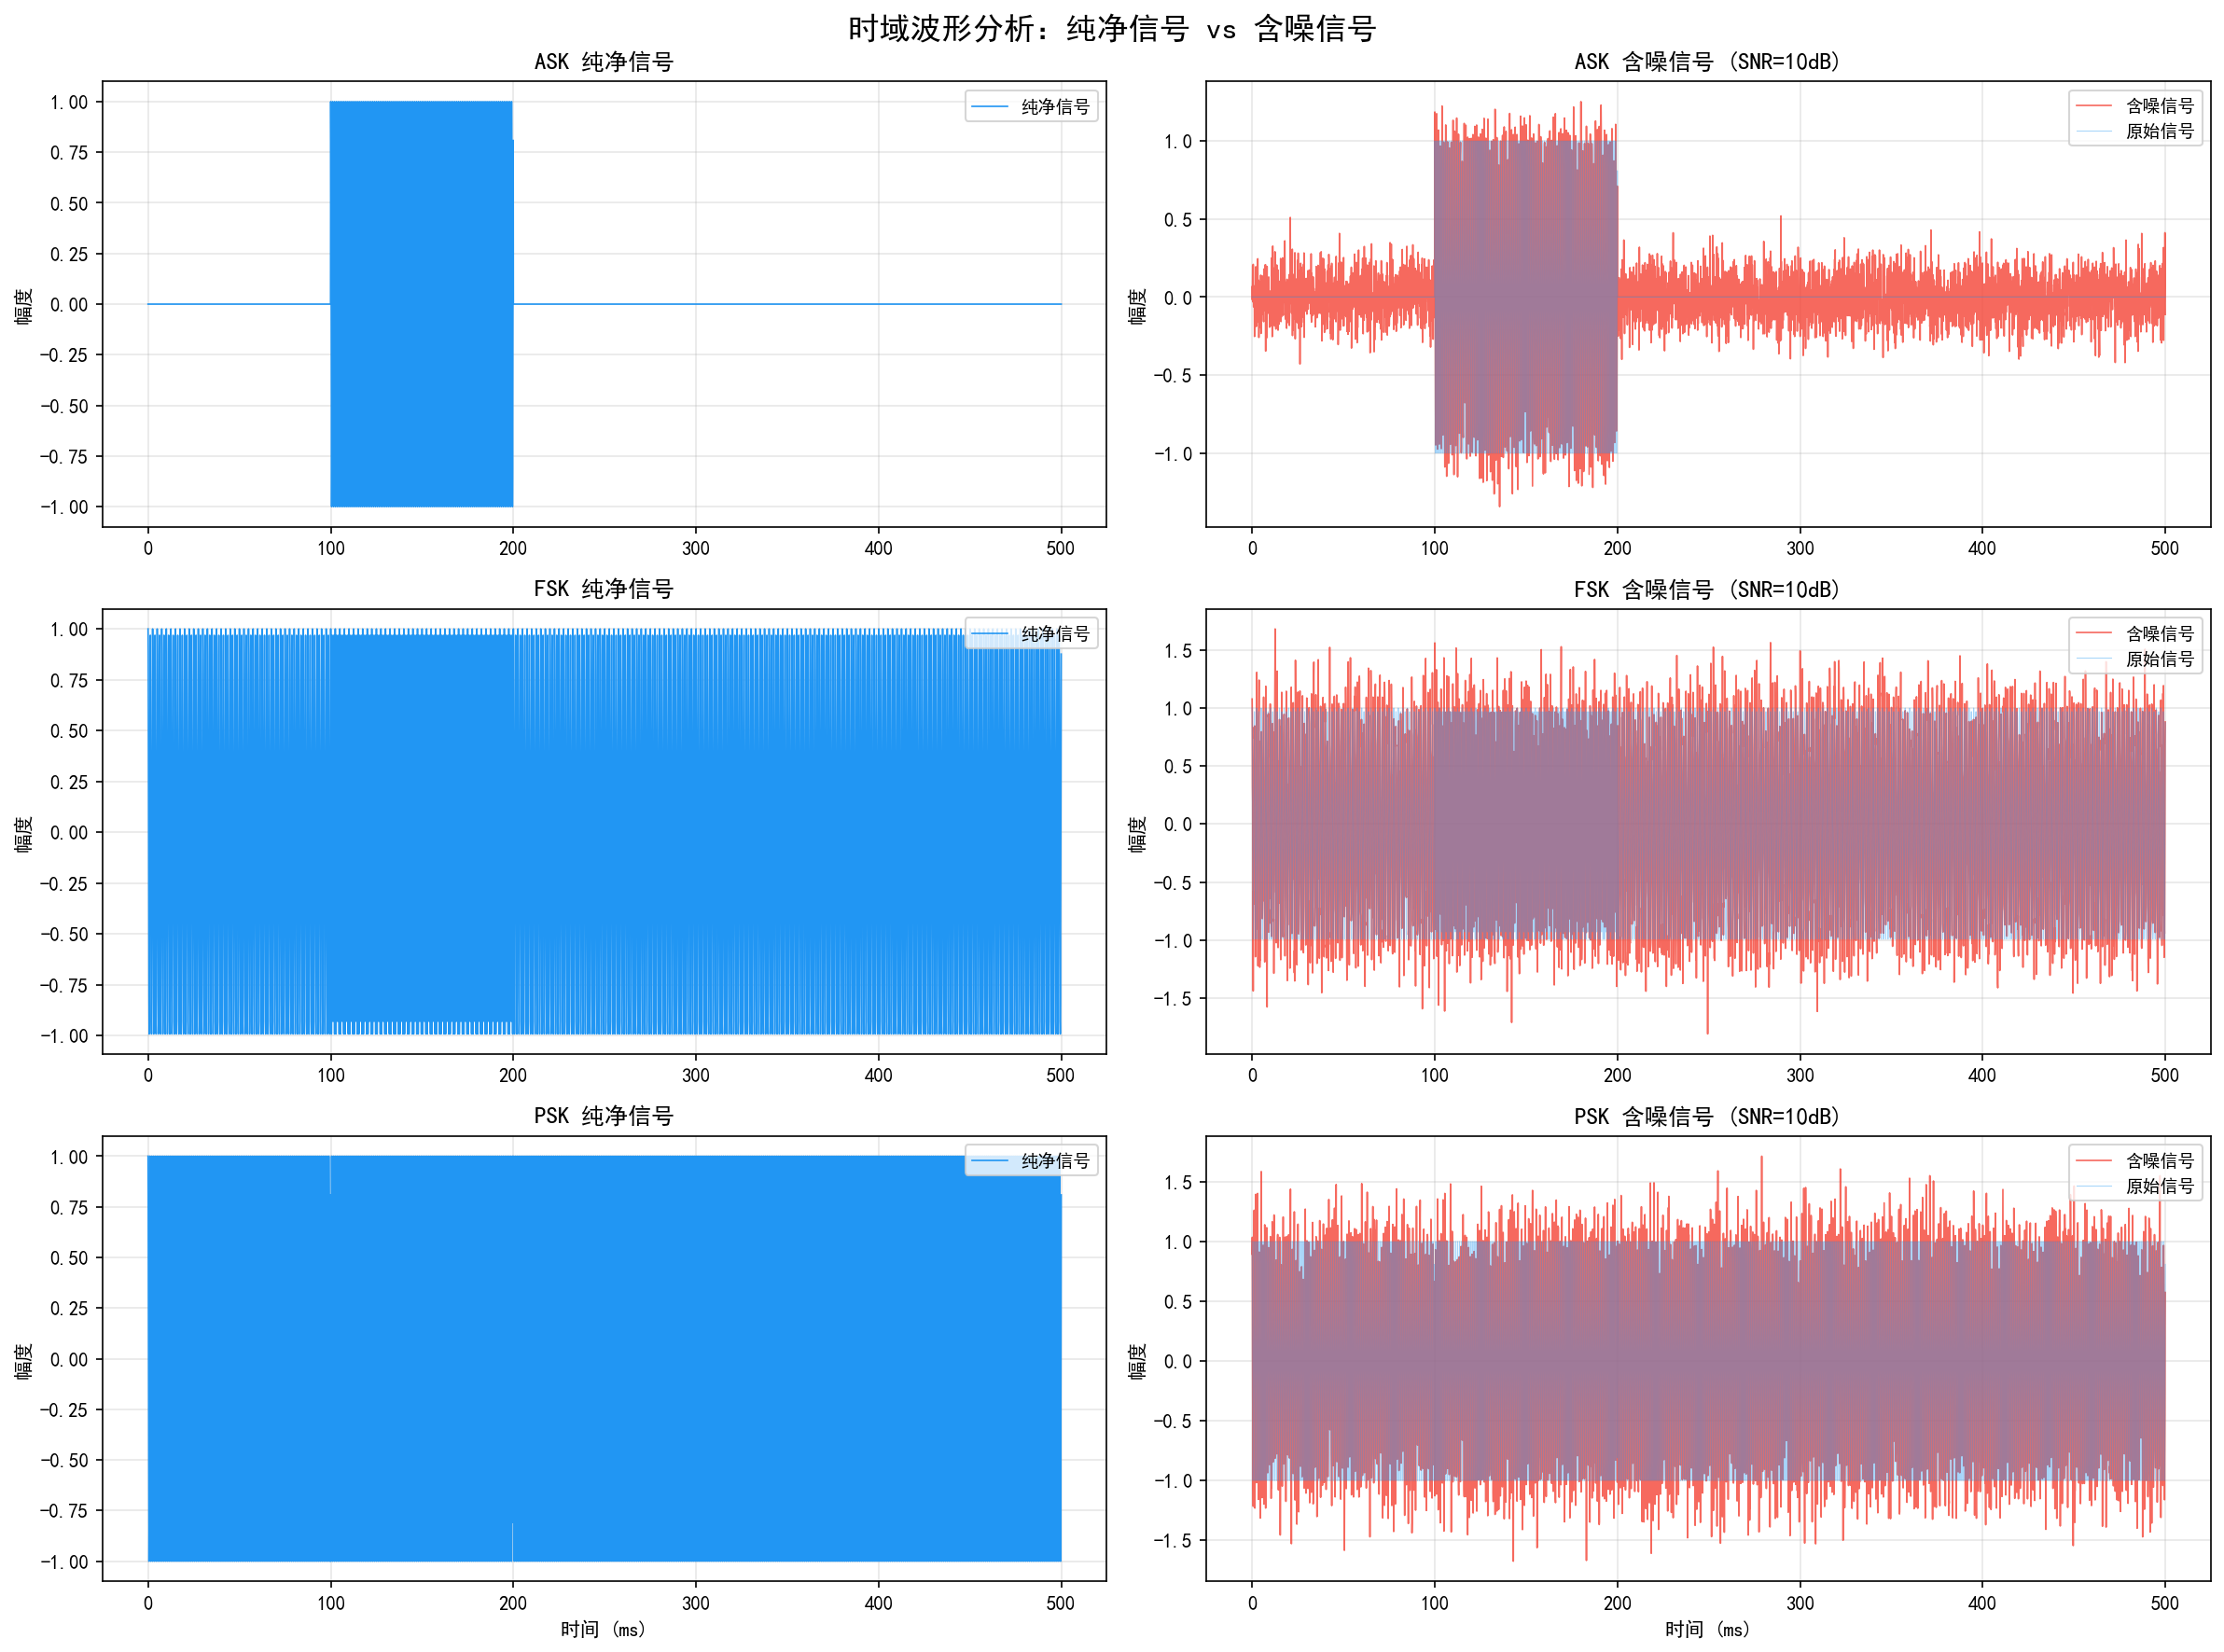
\includegraphics[width=0.85\textwidth]{01_time_domain_signals.png}
\caption{三种调制信号时域波形（纯净 vs 含噪，SNR=10\,dB）}
\label{fig:time}
\end{figure}

\begin{figure}[htbp]
\centering
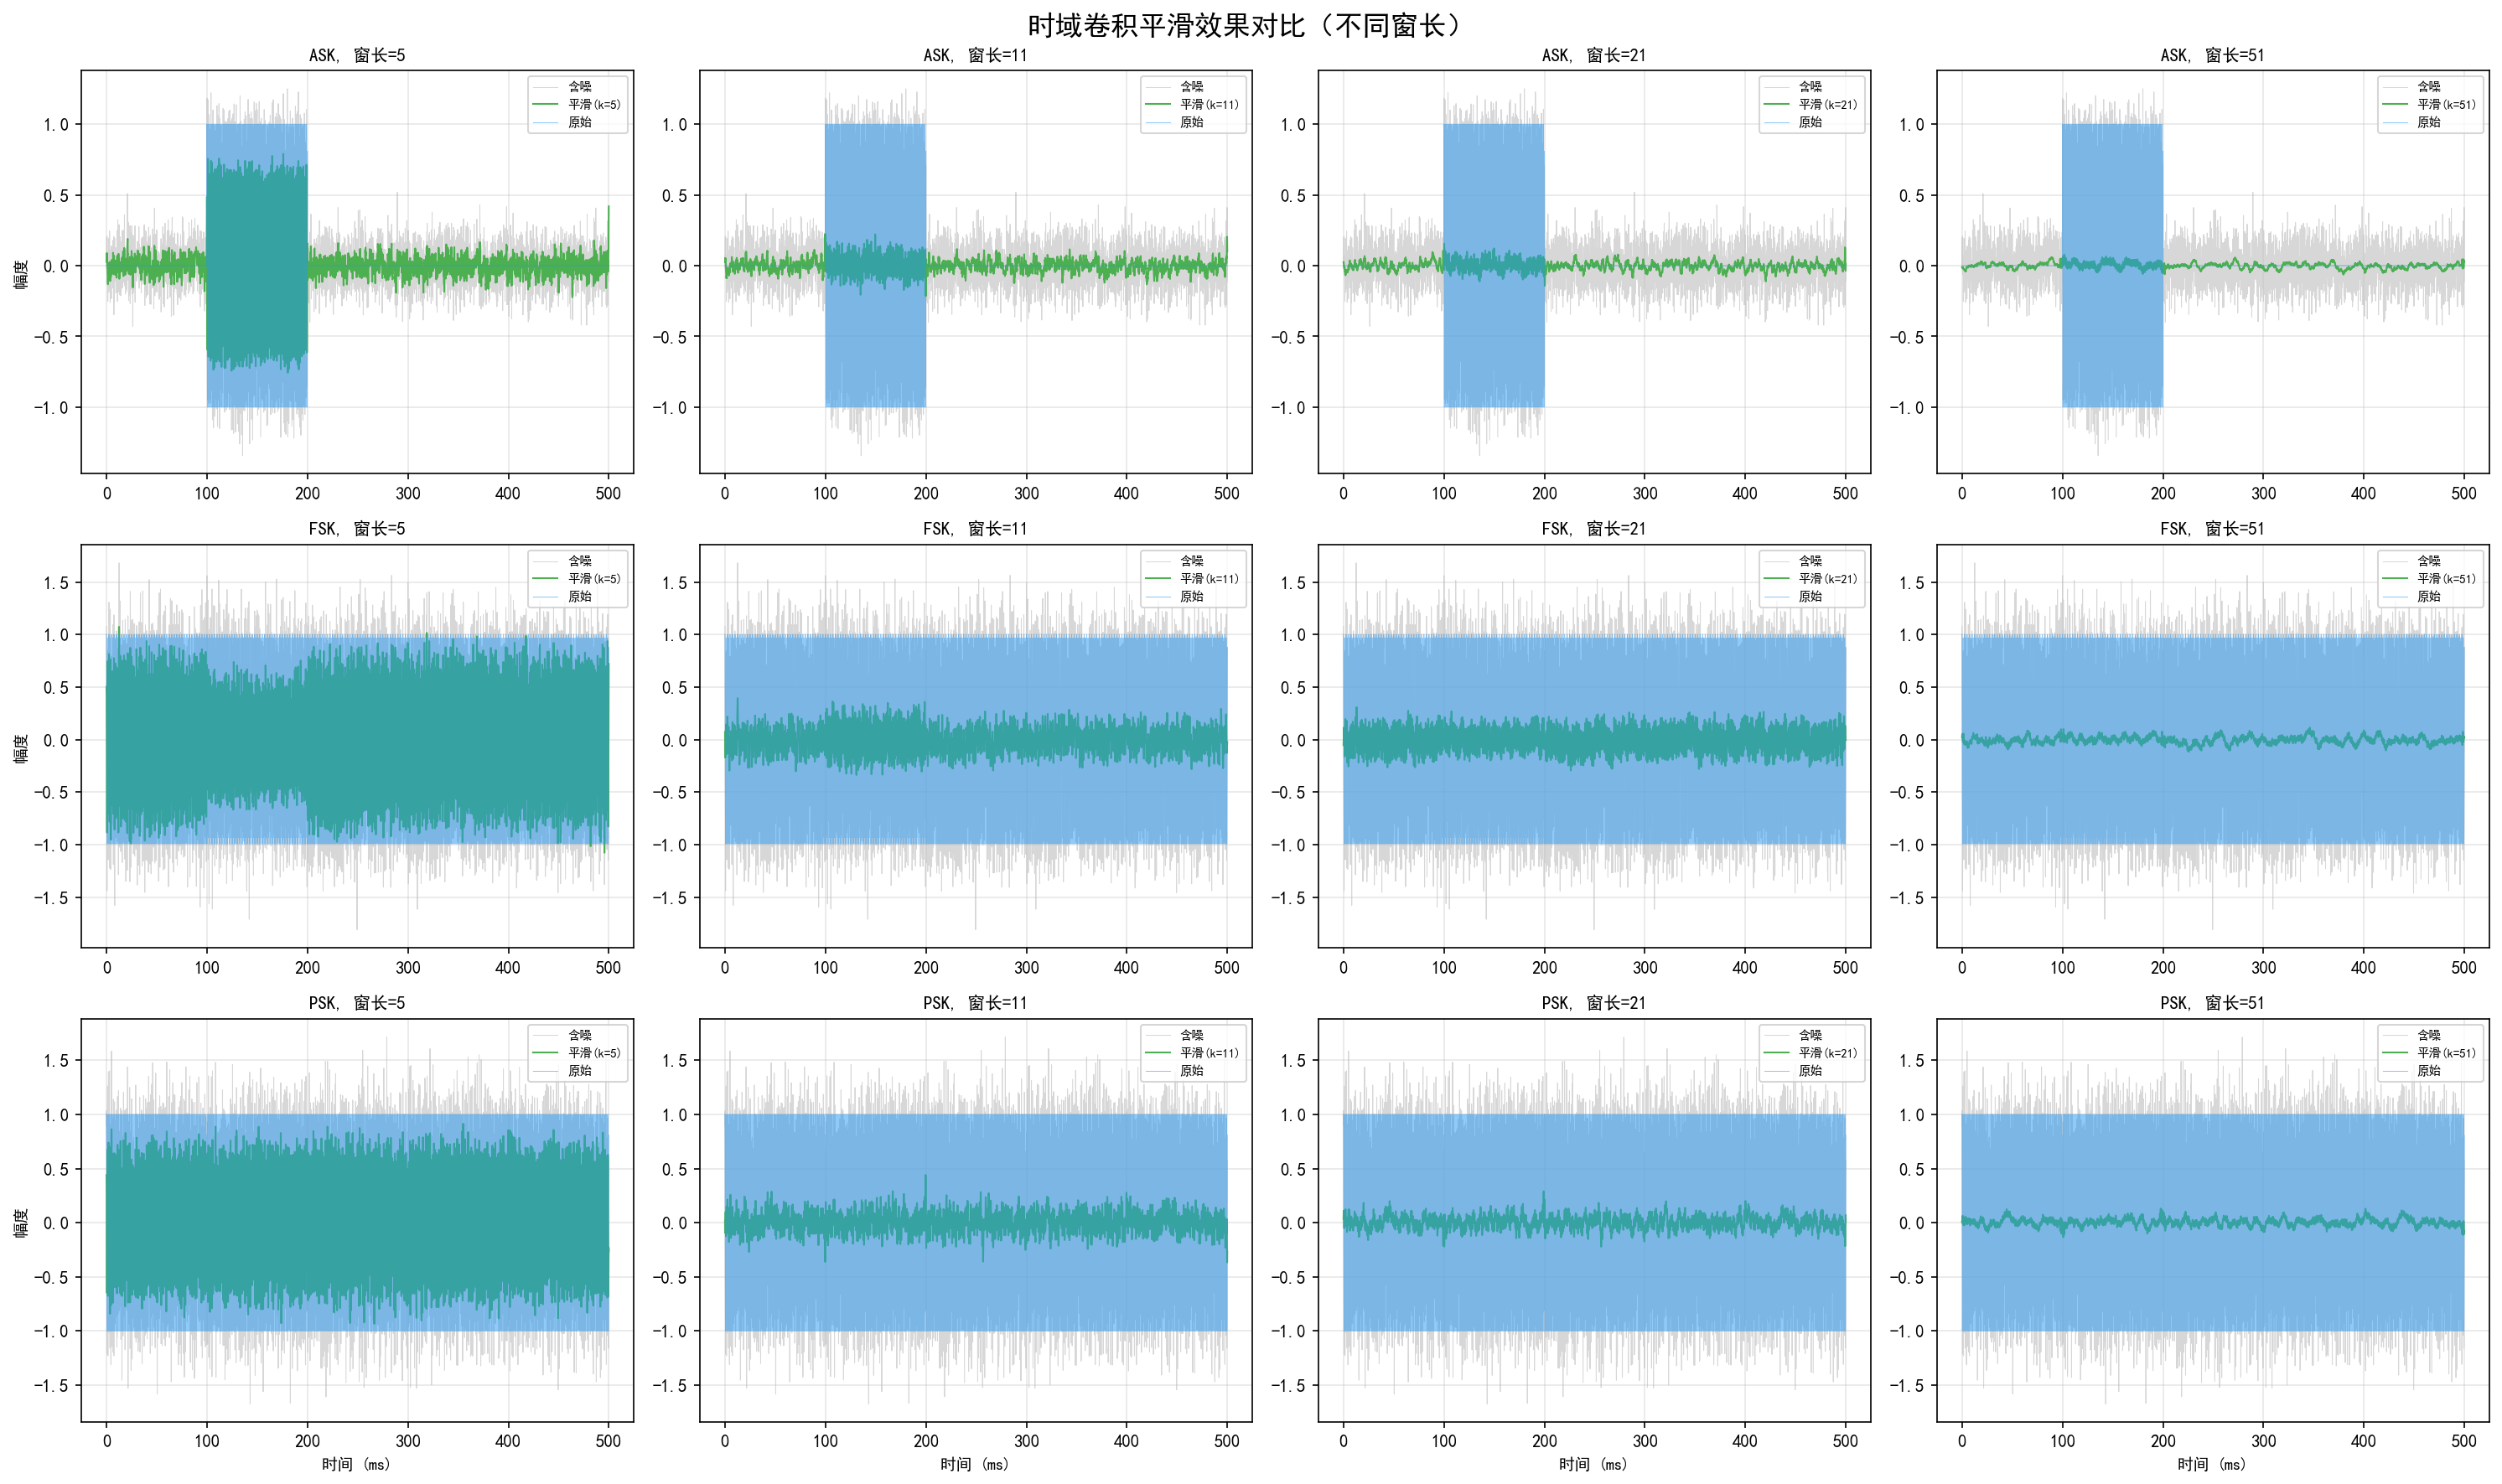
\includegraphics[width=0.88\textwidth]{02_convolution_smooth.png}
\caption{不同窗长的卷积平滑效果对比}
\label{fig:smooth}
\end{figure}

\subsection{多变换域联合分析}

图~\ref{fig:dft}--\ref{fig:zp} 分别为 DFT 幅度/相位谱、DTFT 连续谱与 Z 域零极点分布。DFT 频域中 FSK 呈现间隔 400\,Hz 的双峰，ASK/PSK 为单峰；Z 域中三种信号的强极点均落在各自载频对应角度附近。图~\ref{fig:cmp15} 将 DFT 谱线叠加在 DTFT 连续谱上，直观展示``DFT 是 DTFT 的等间隔采样''（谱线间隔 $F_s/N=0.5$\,Hz）；图~\ref{fig:multi} 为时域--频域--Z 域三列联合对比总览。

\begin{figure}[htbp]
\centering
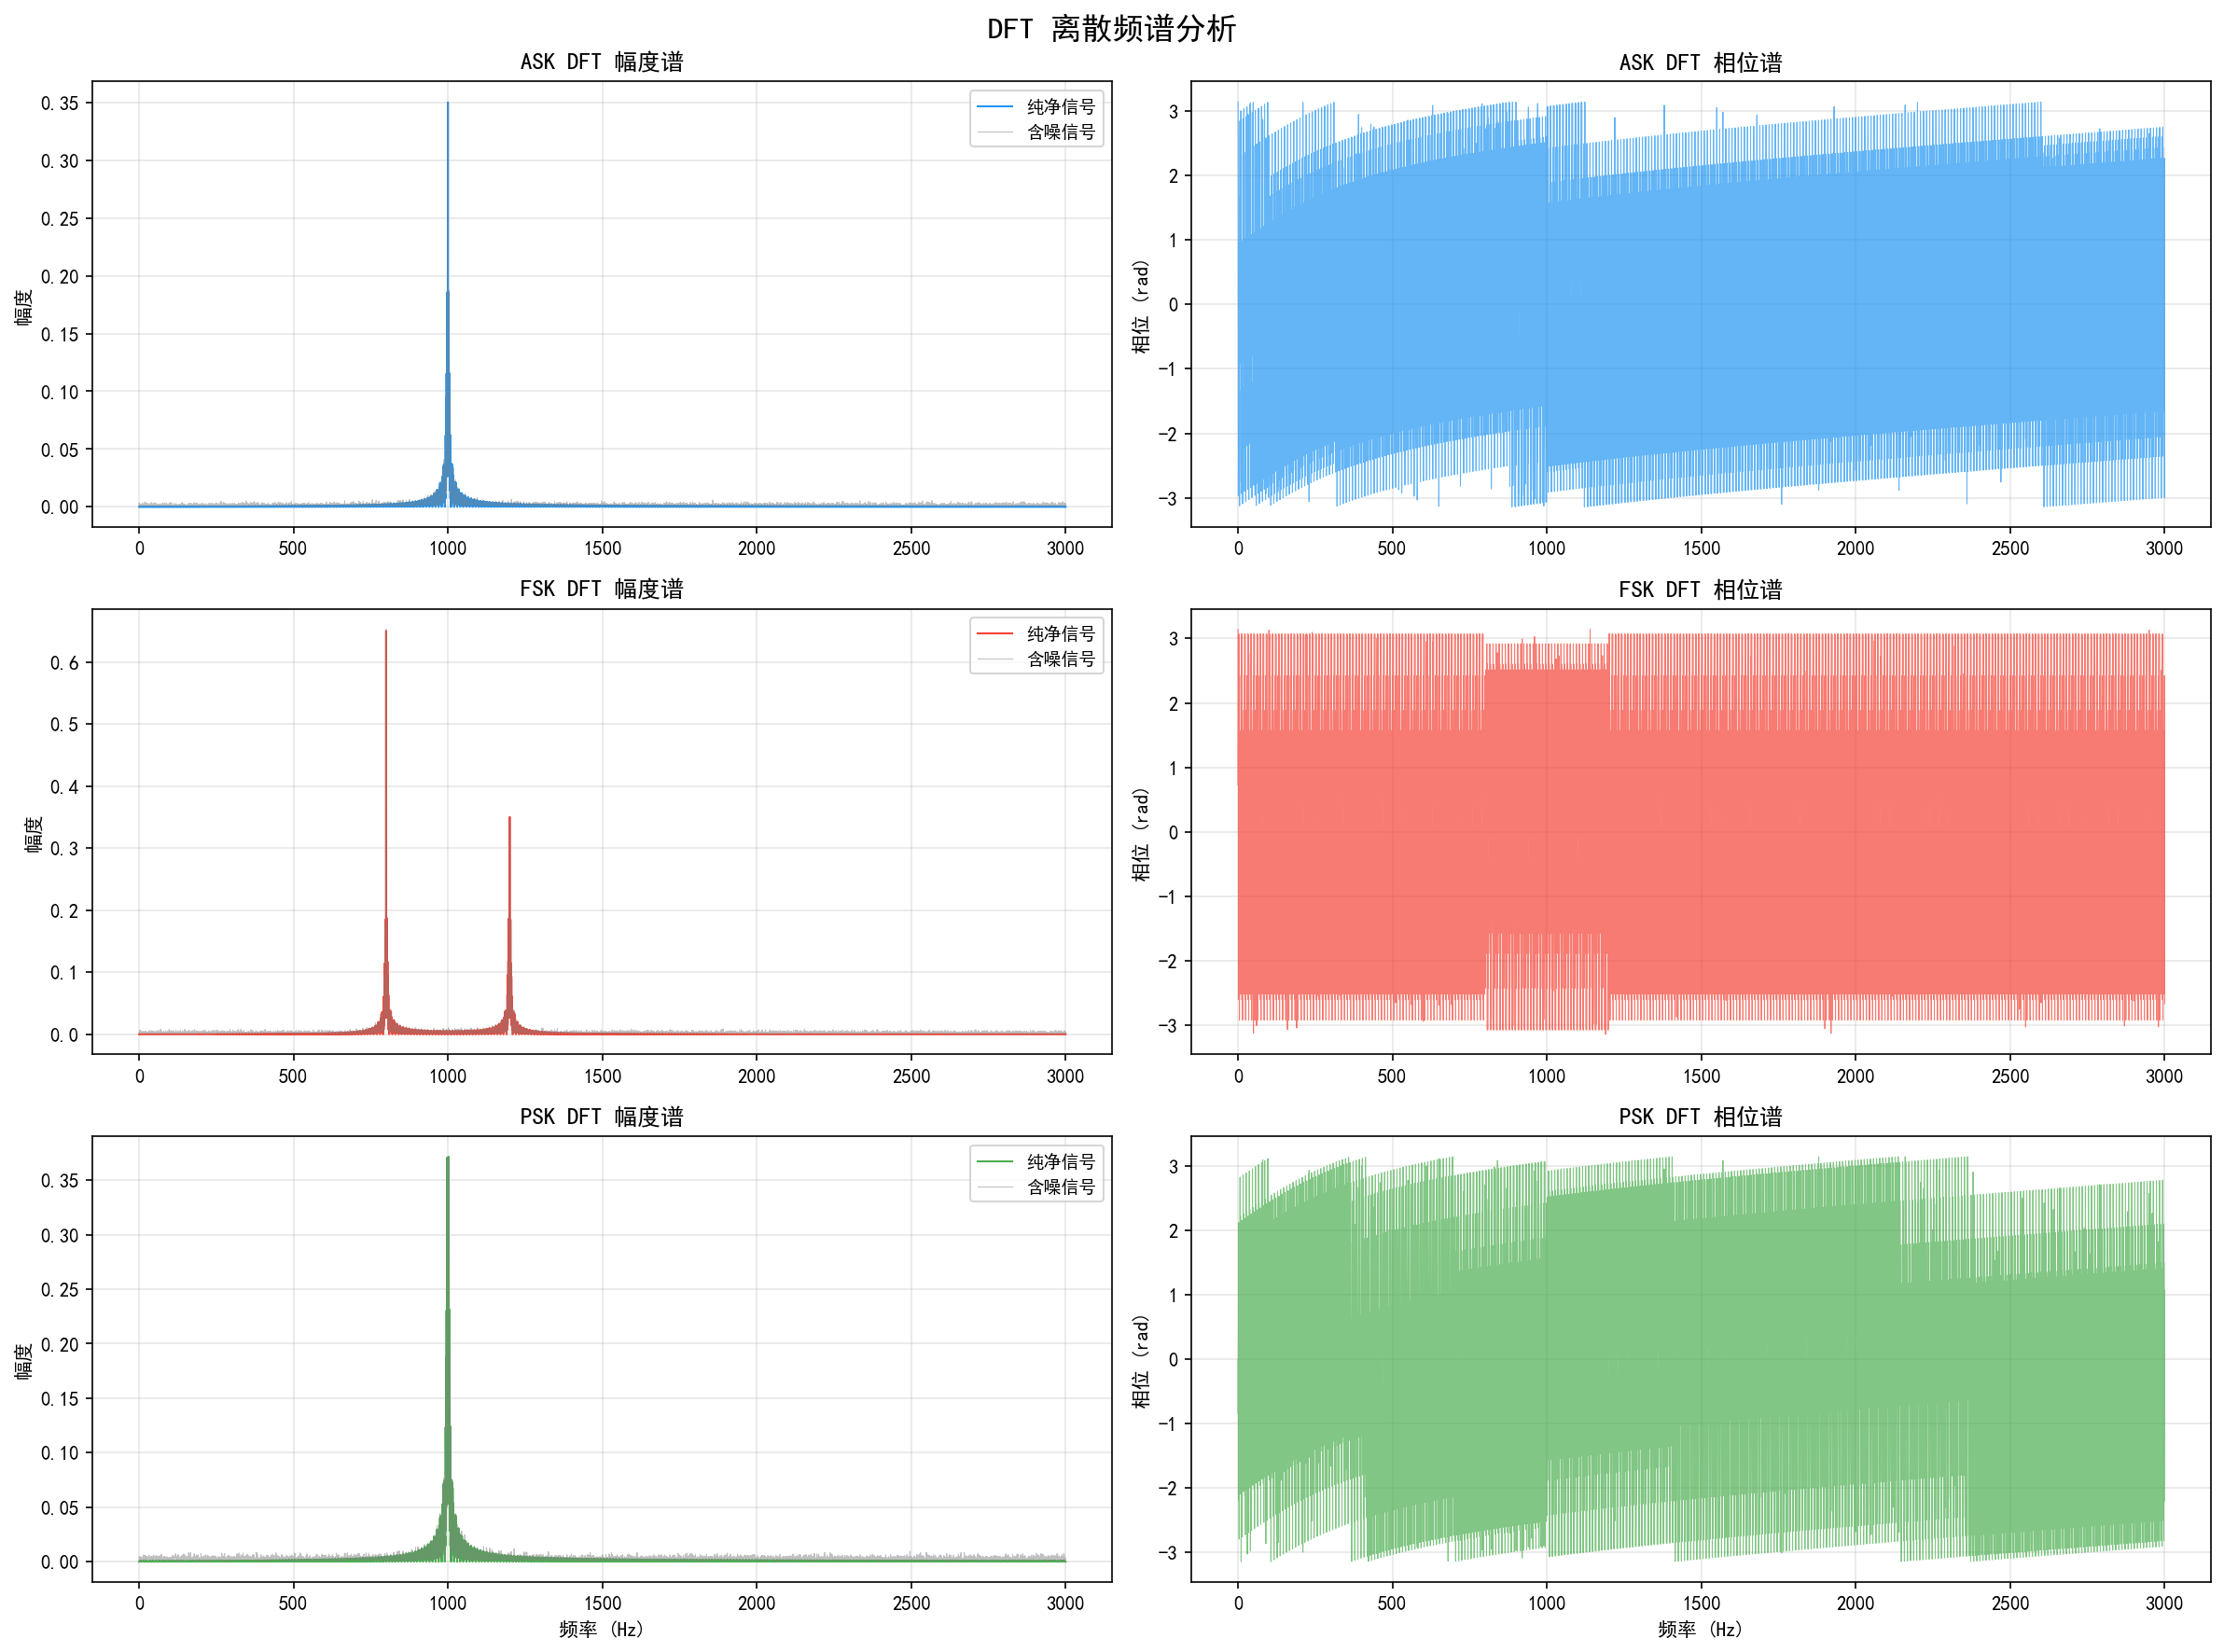
\includegraphics[width=0.88\textwidth]{03_dft_spectrum.png}
\caption{DFT 离散频谱（左：幅度谱，右：相位谱）}
\label{fig:dft}
\end{figure}

\begin{figure}[htbp]
\centering
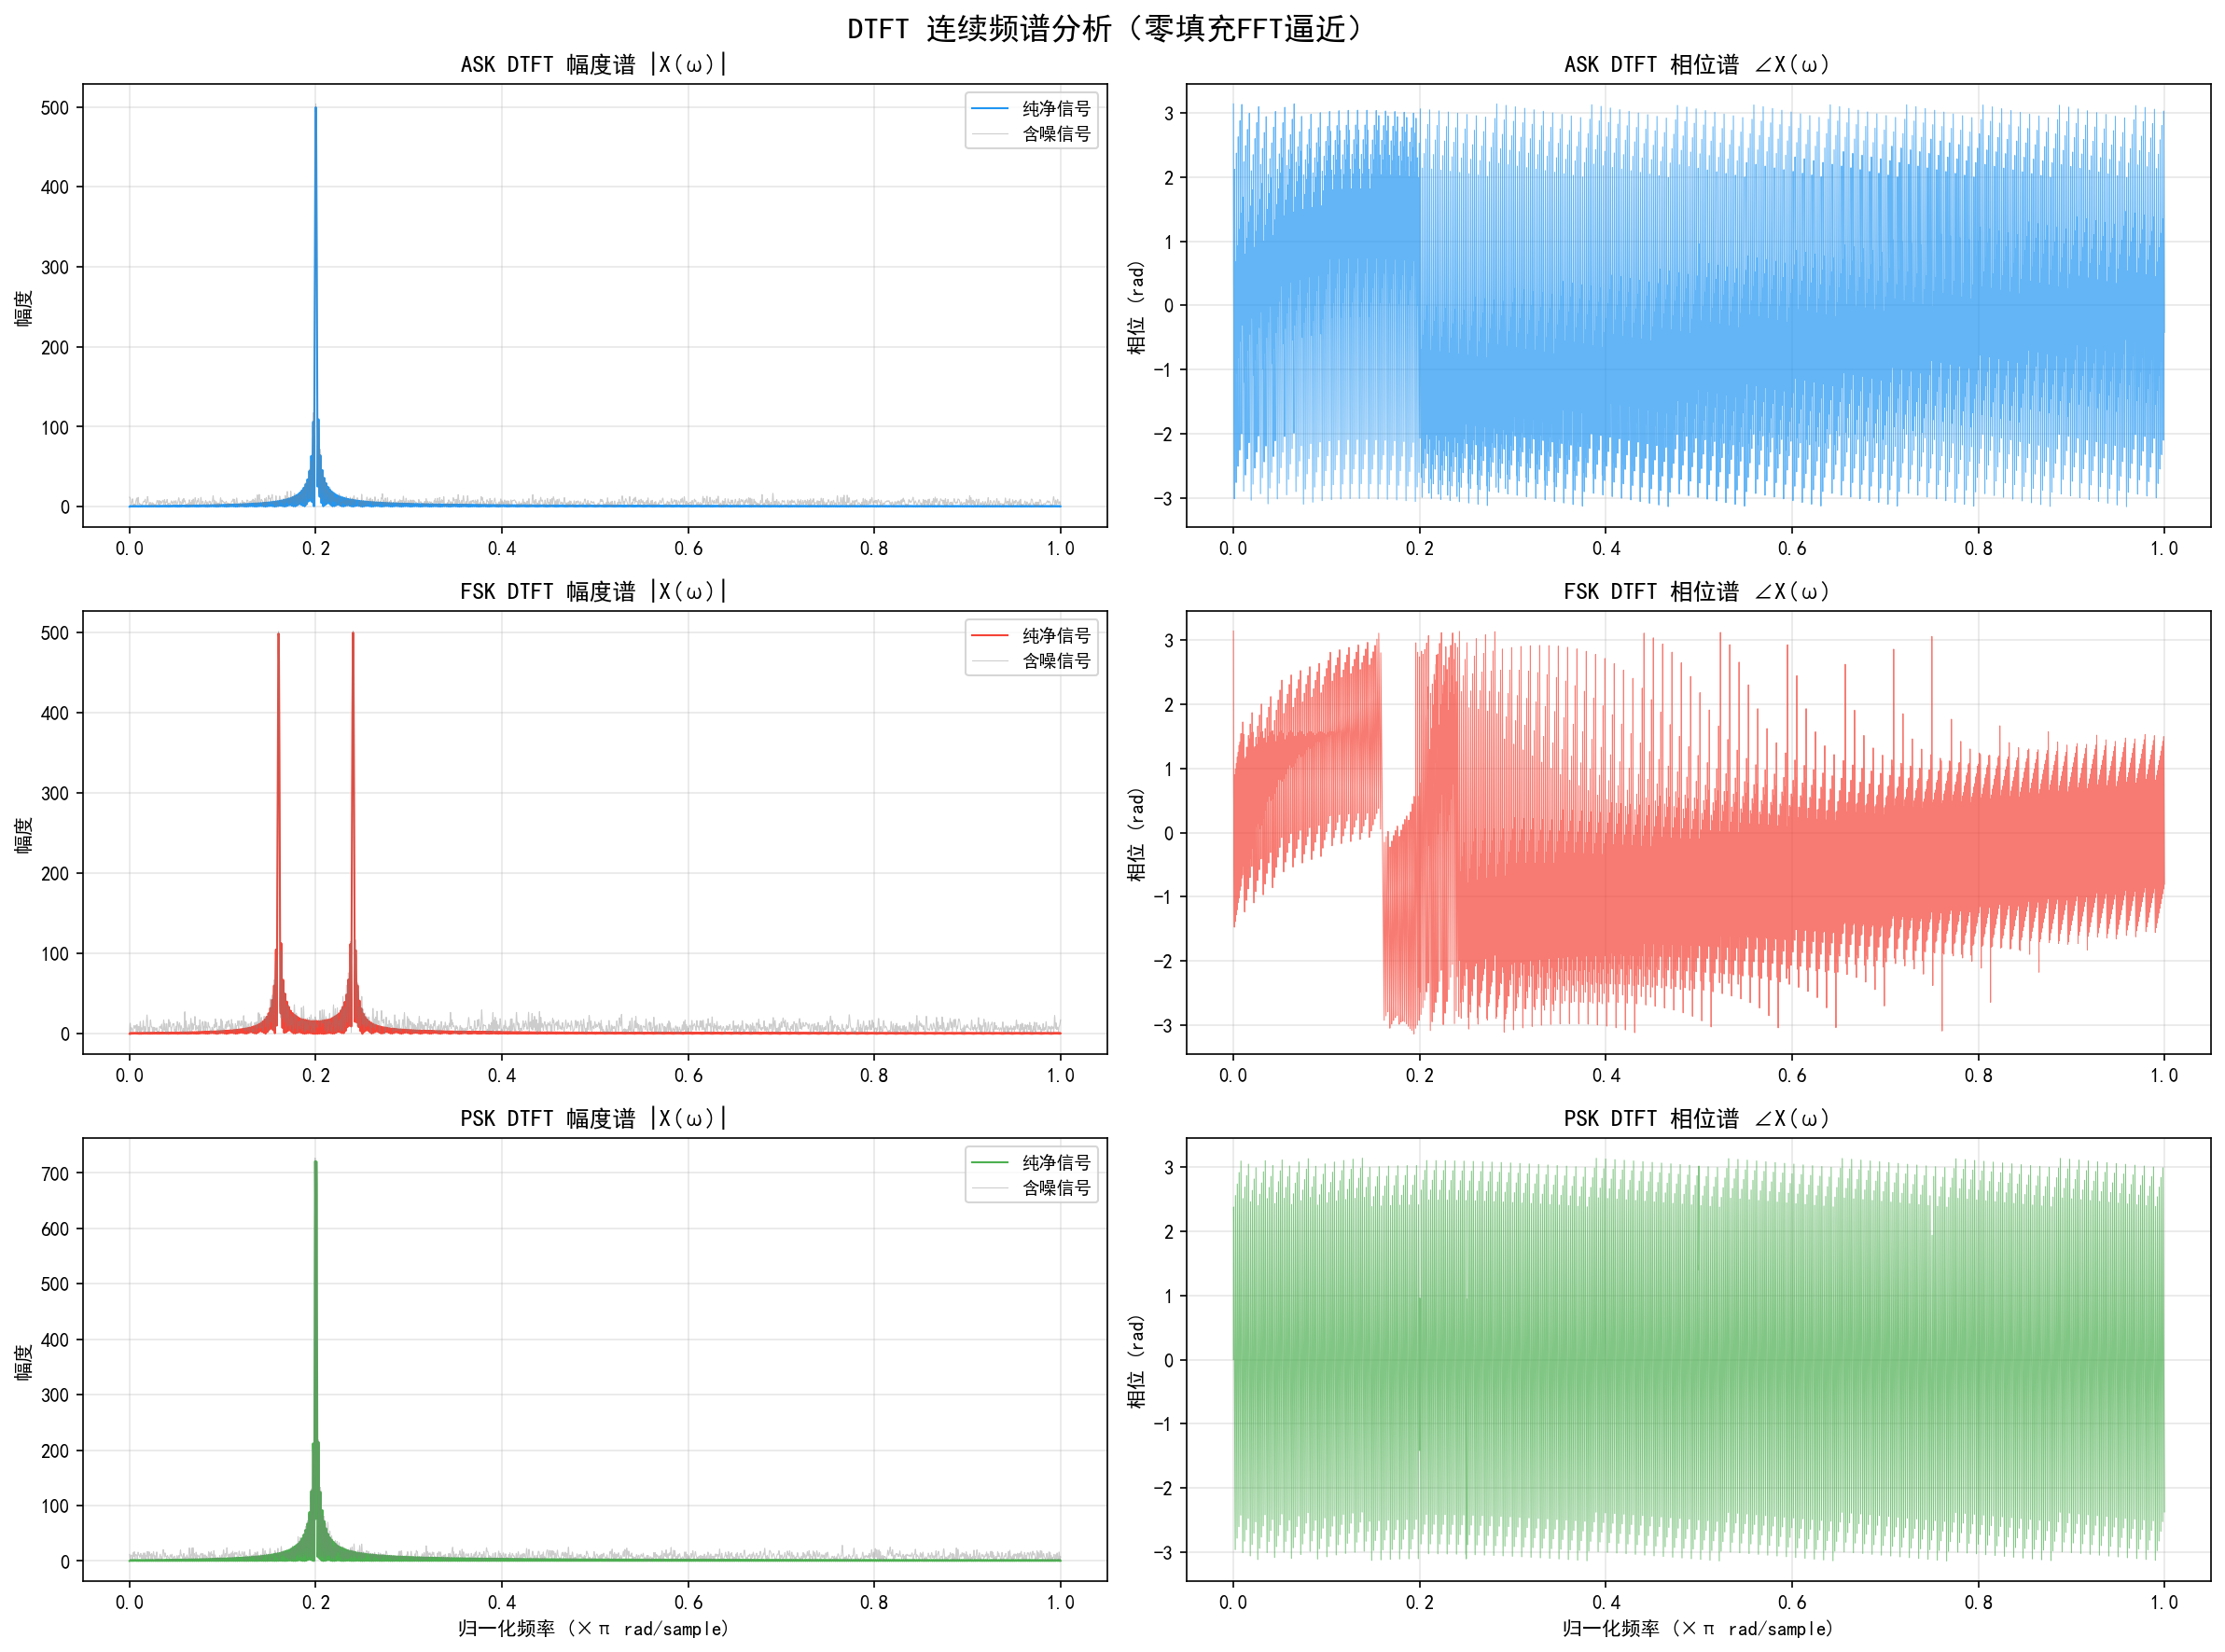
\includegraphics[width=0.88\textwidth]{04_dtft_spectrum.png}
\caption{DTFT 连续频谱（零填充 FFT 逼近）}
\label{fig:dtft}
\end{figure}

\begin{figure}[htbp]
\centering
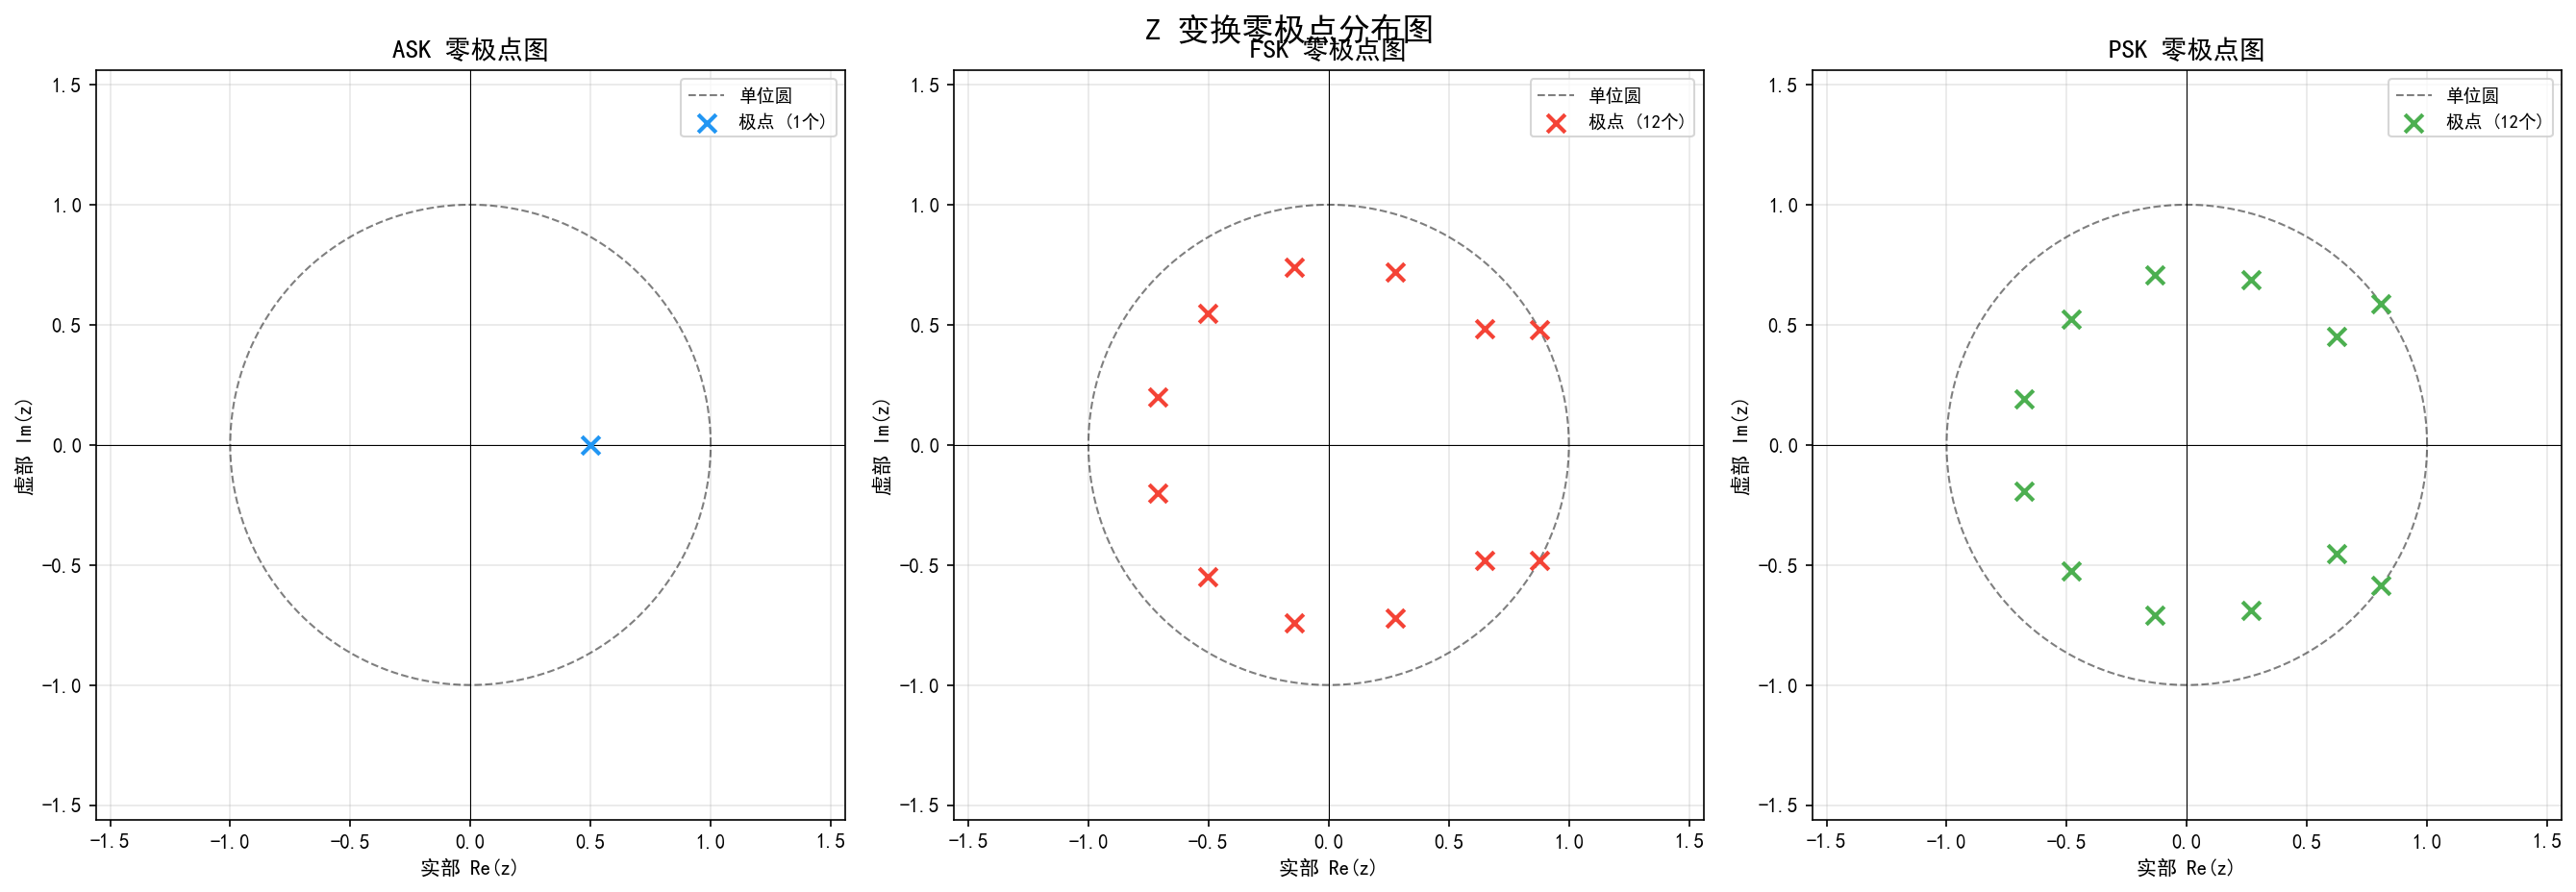
\includegraphics[width=0.95\textwidth]{05_zero_pole_map.png}
\caption{Z 变换零极点分布（AR 模型建模）}
\label{fig:zp}
\end{figure}

\begin{figure}[htbp]
\centering
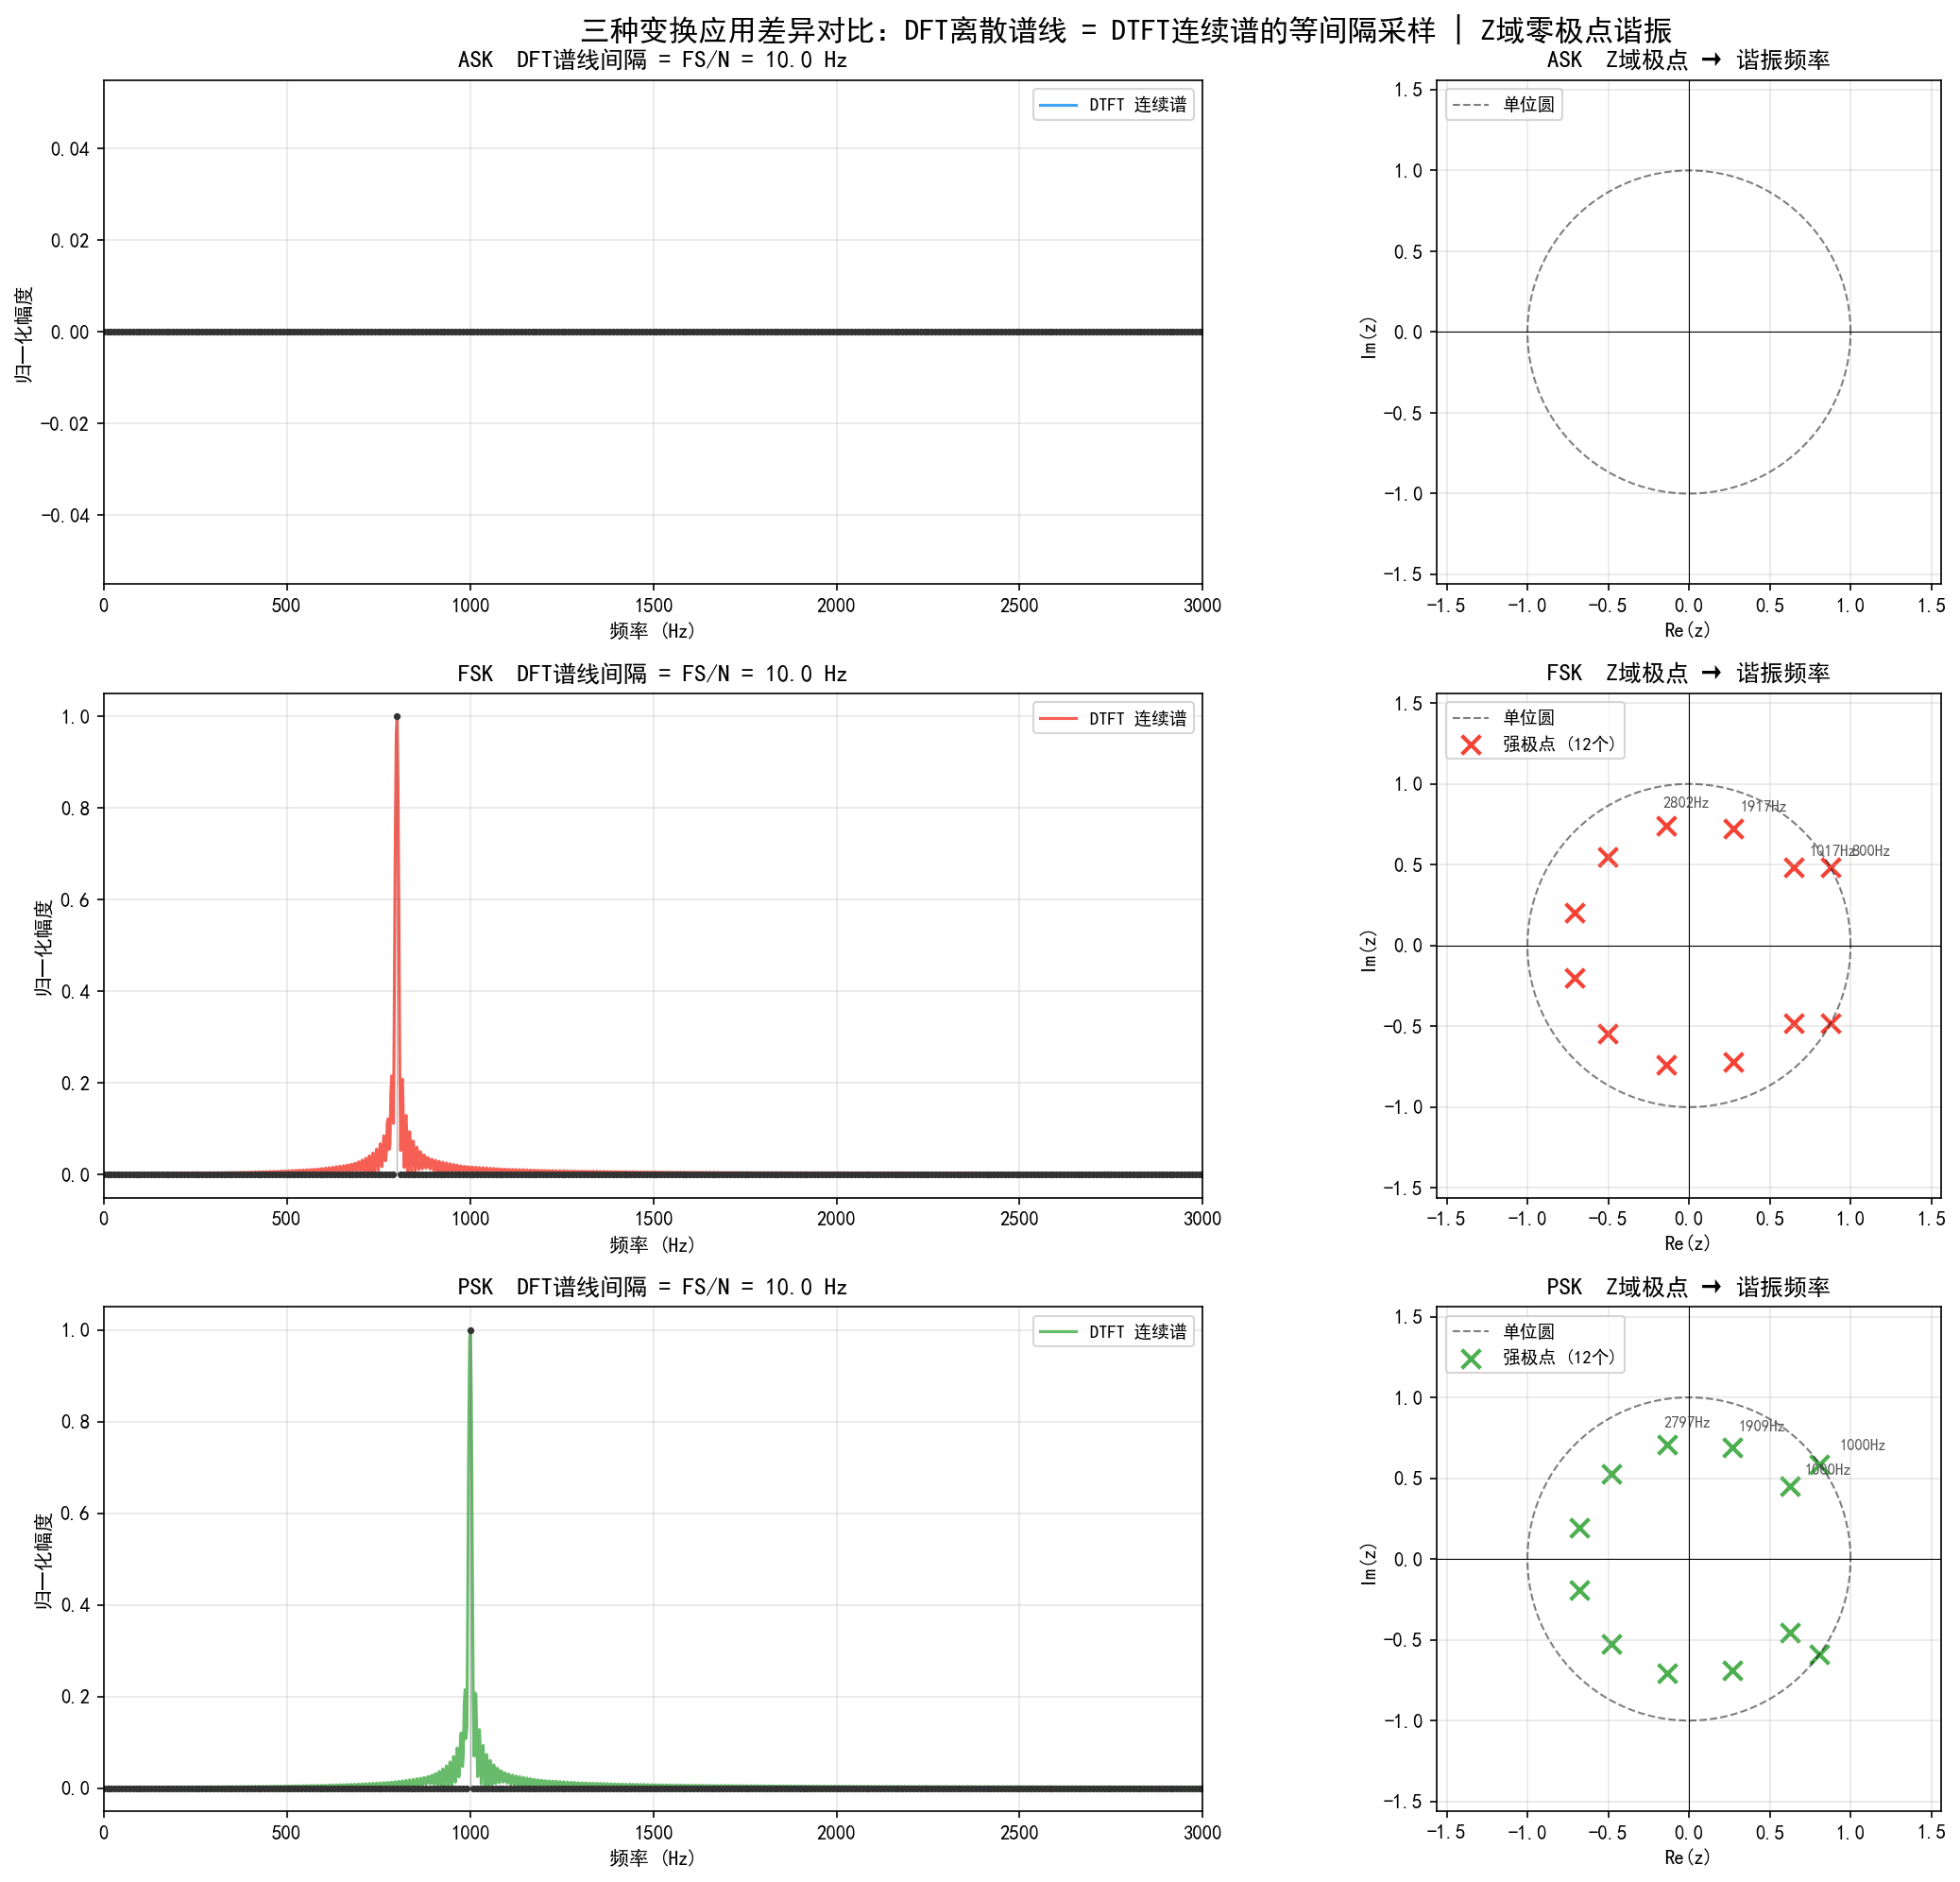
\includegraphics[width=0.8\textwidth]{15_transform_comparison.png}
\caption{三种变换应用差异对比：DFT 谱线与 DTFT 连续谱的采样关系（左），Z 域极点谐振频率（右）}
\label{fig:cmp15}
\end{figure}

\begin{figure}[htbp]
\centering
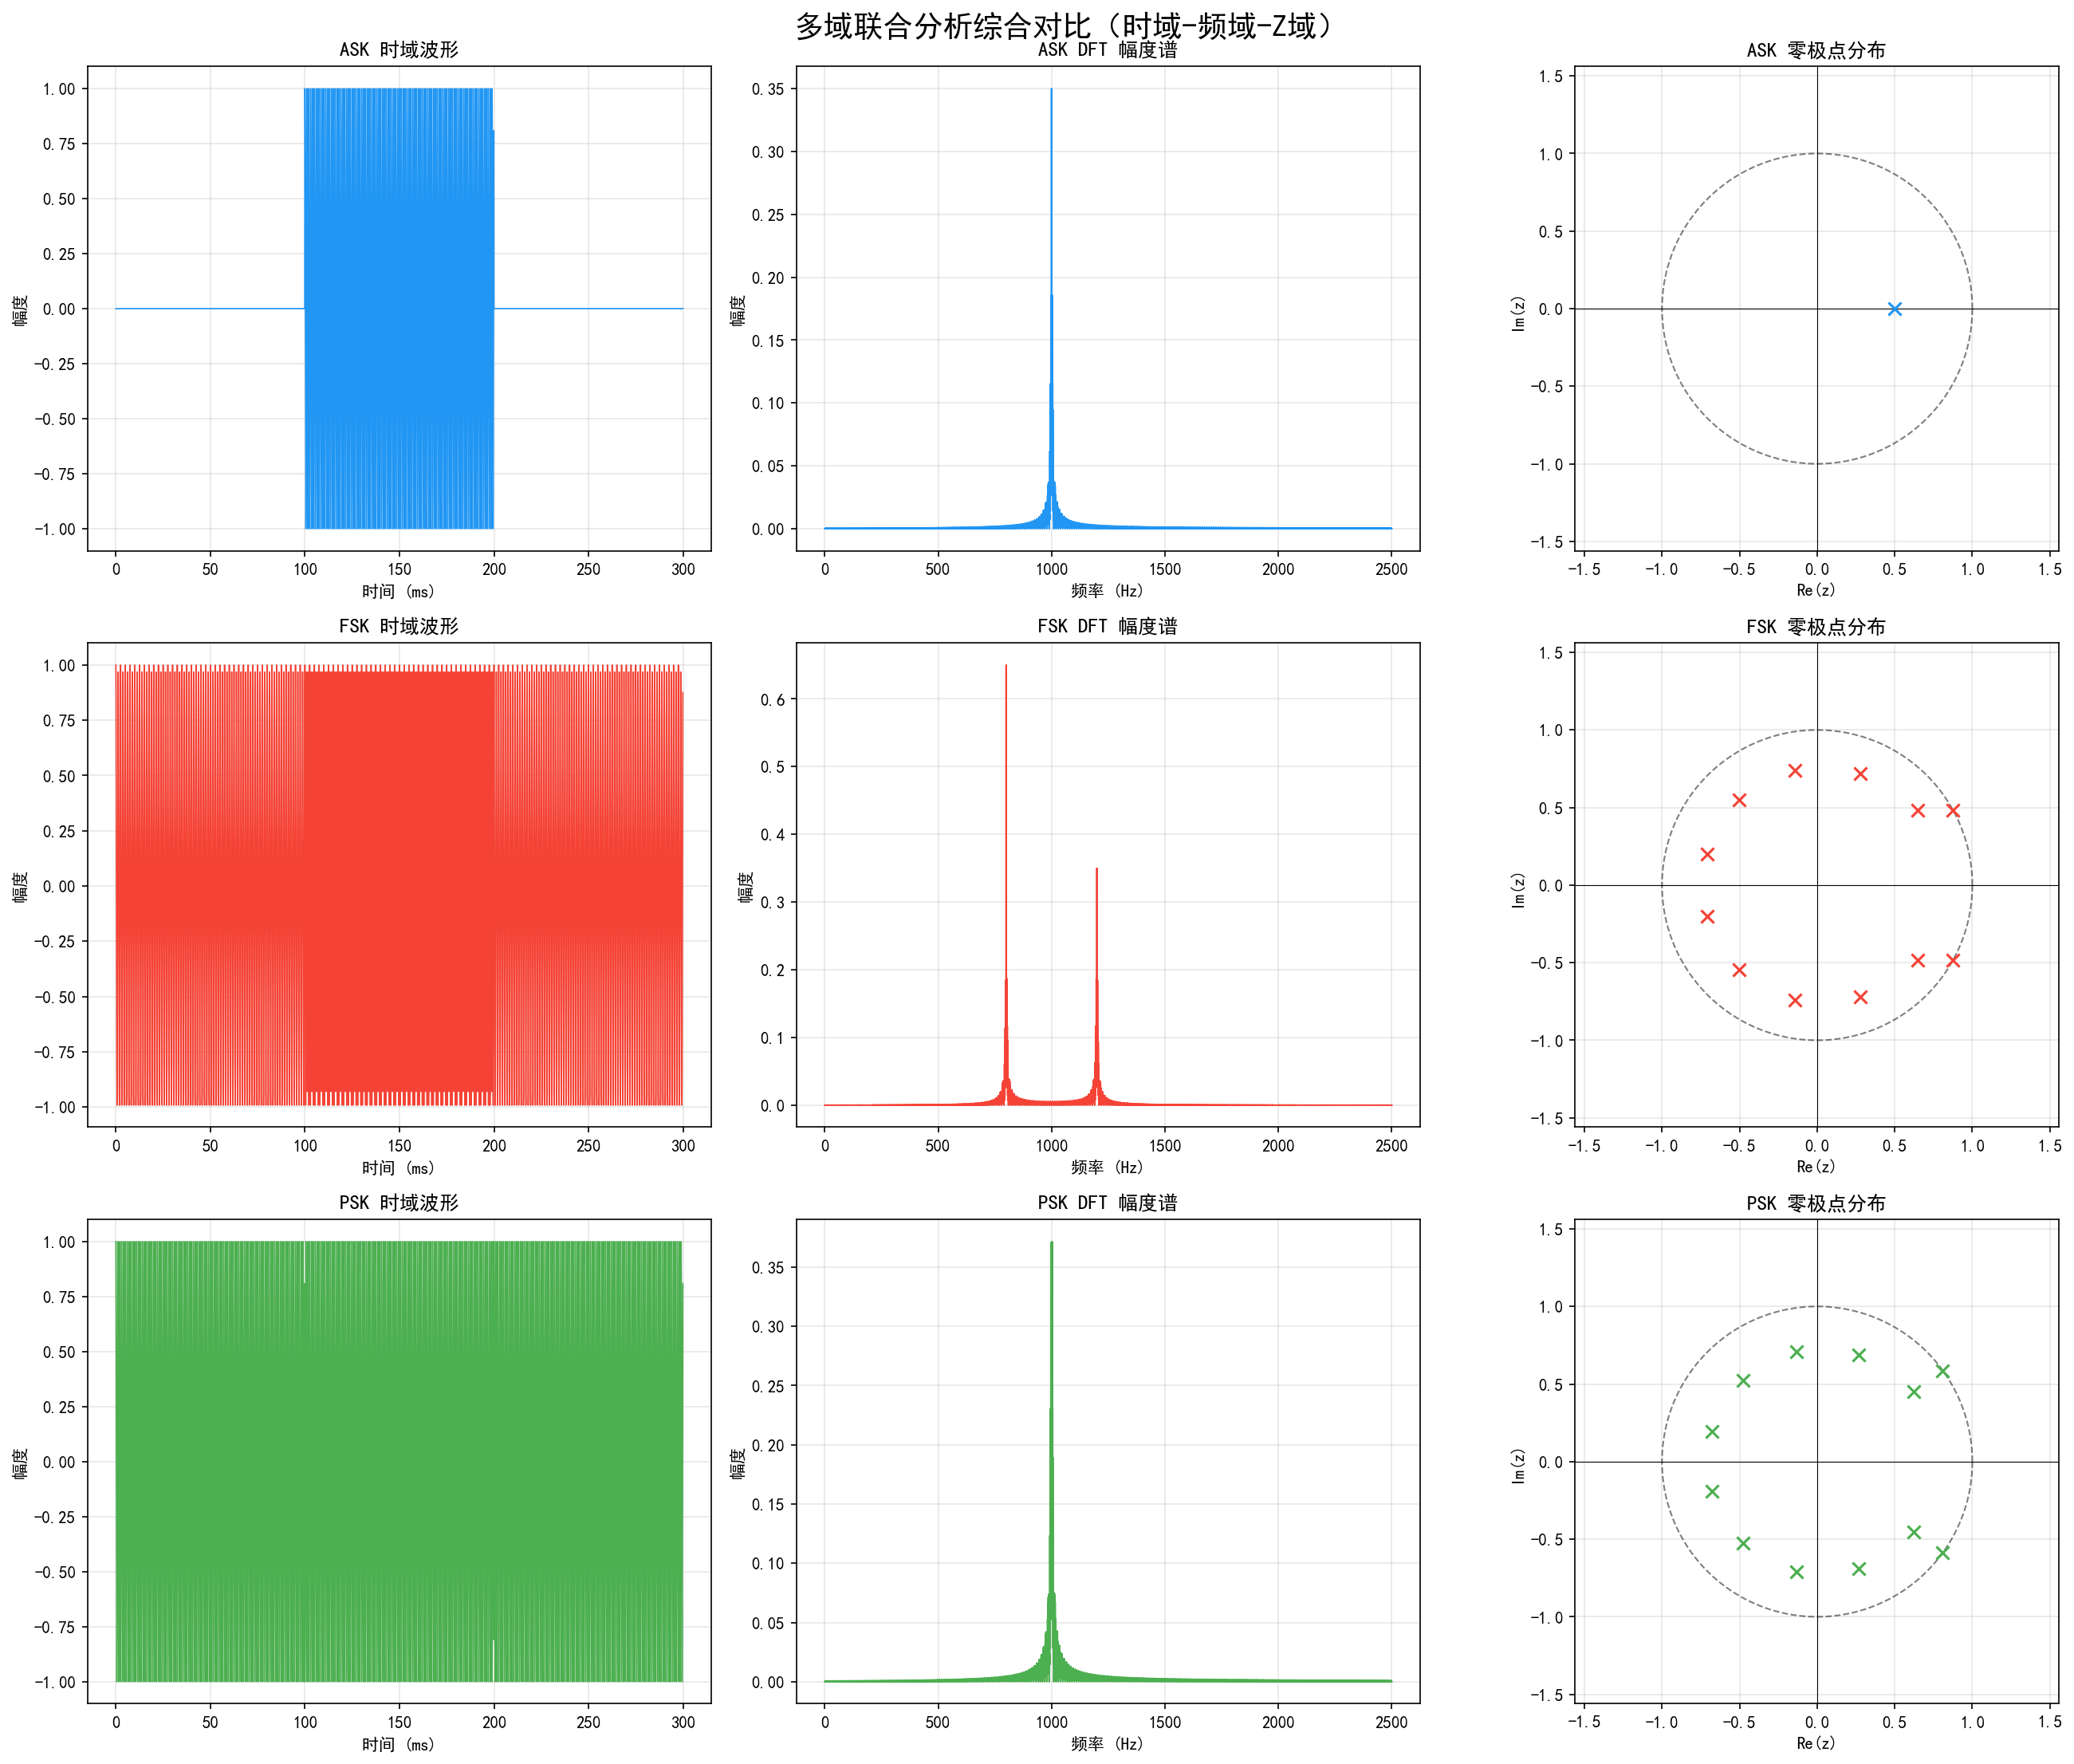
\includegraphics[width=0.78\textwidth]{13_multi_domain_comparison.png}
\caption{时域--频域--Z 域多域联合对比总览}
\label{fig:multi}
\end{figure}

\subsection{滤波器设计与迭代优化}

以 FSK 带通（500--1500\,Hz）为例，FIR（64 阶 Hamming）与 IIR（4 阶 Butterworth）的幅频/相频特性如图~\ref{fig:firiir}。FIR 严格线性相位；IIR 阶数低、过渡带窄但相位非线性——系统采用 filtfilt 零相位滤波消除其影响。IIR 系统函数推导输出示例（$N(z)/D(z)$ 多项式形式）由程序自动打印。

\begin{figure}[htbp]
\centering
\begin{minipage}{0.48\textwidth}
\centering
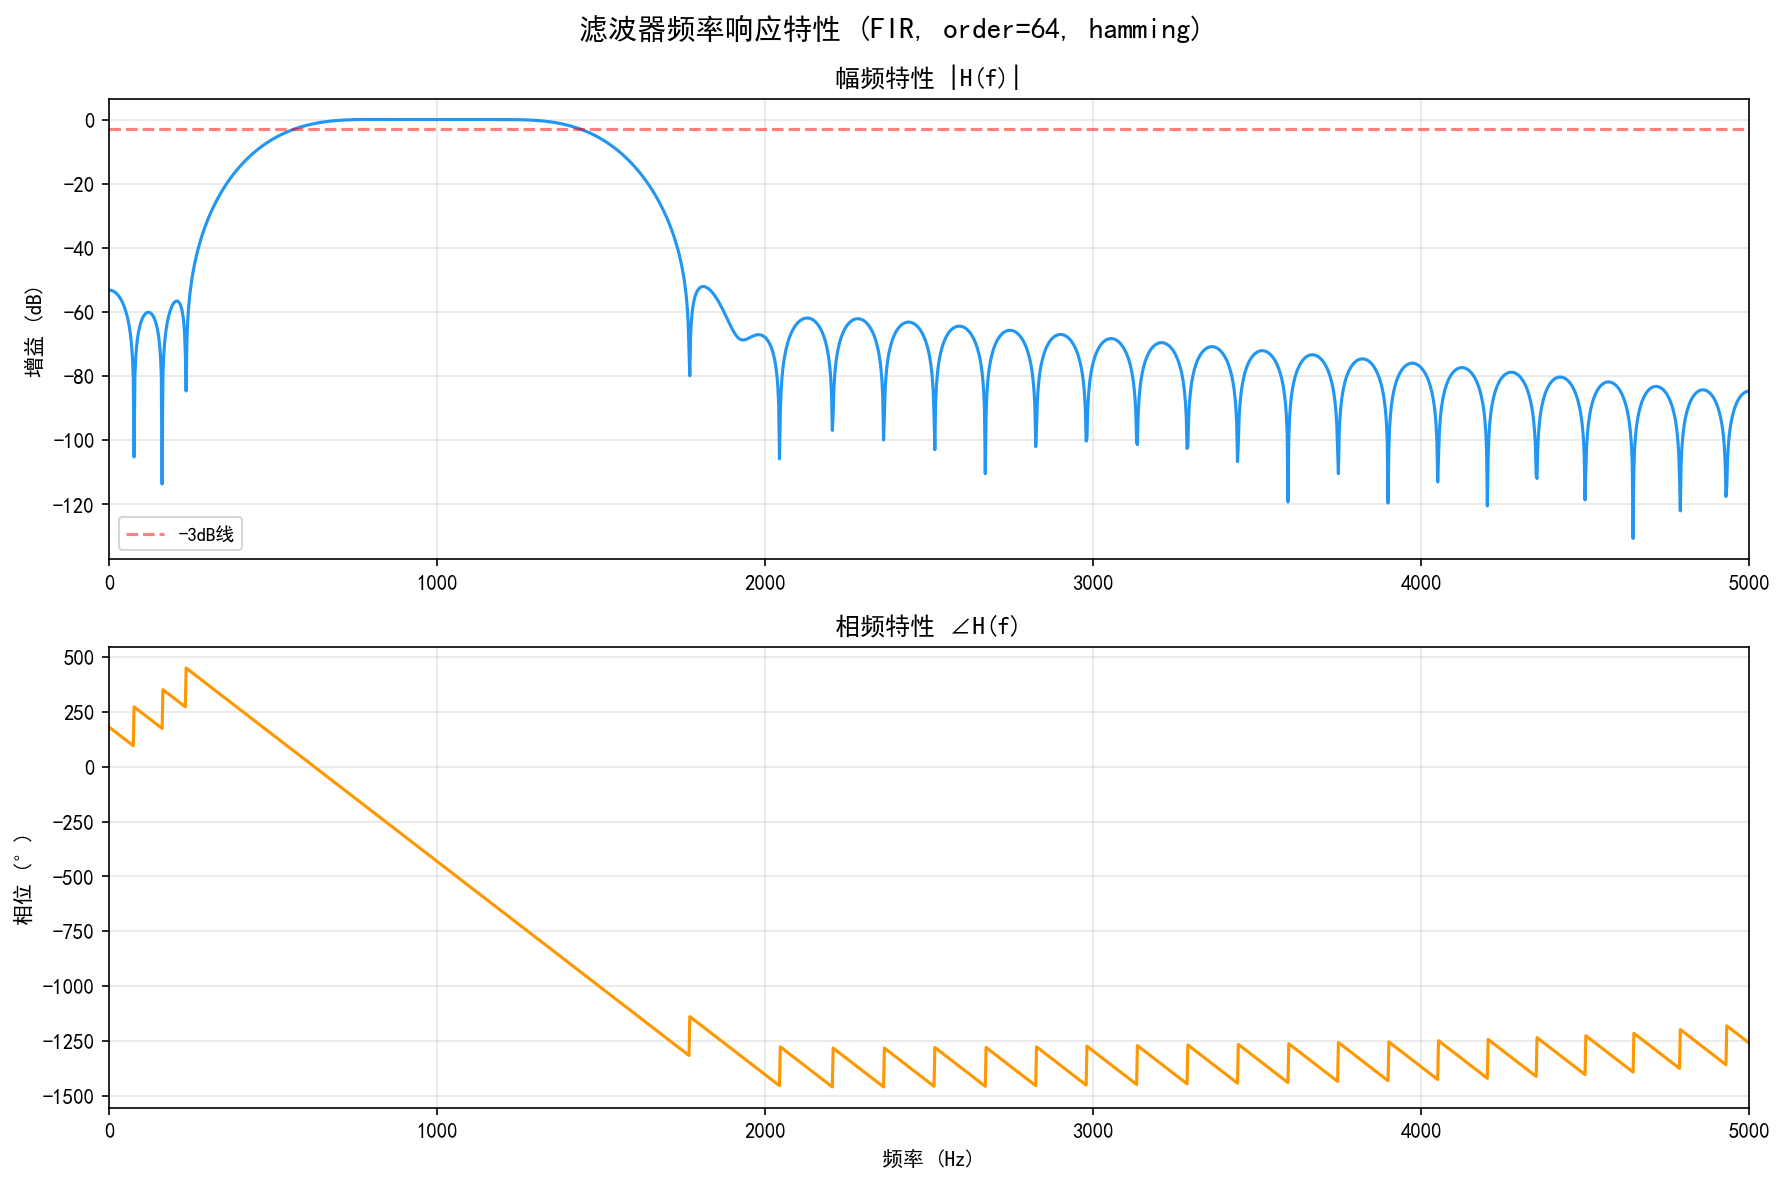
\includegraphics[width=\textwidth]{06_fir_response.png}
\end{minipage}\hfill
\begin{minipage}{0.48\textwidth}
\centering
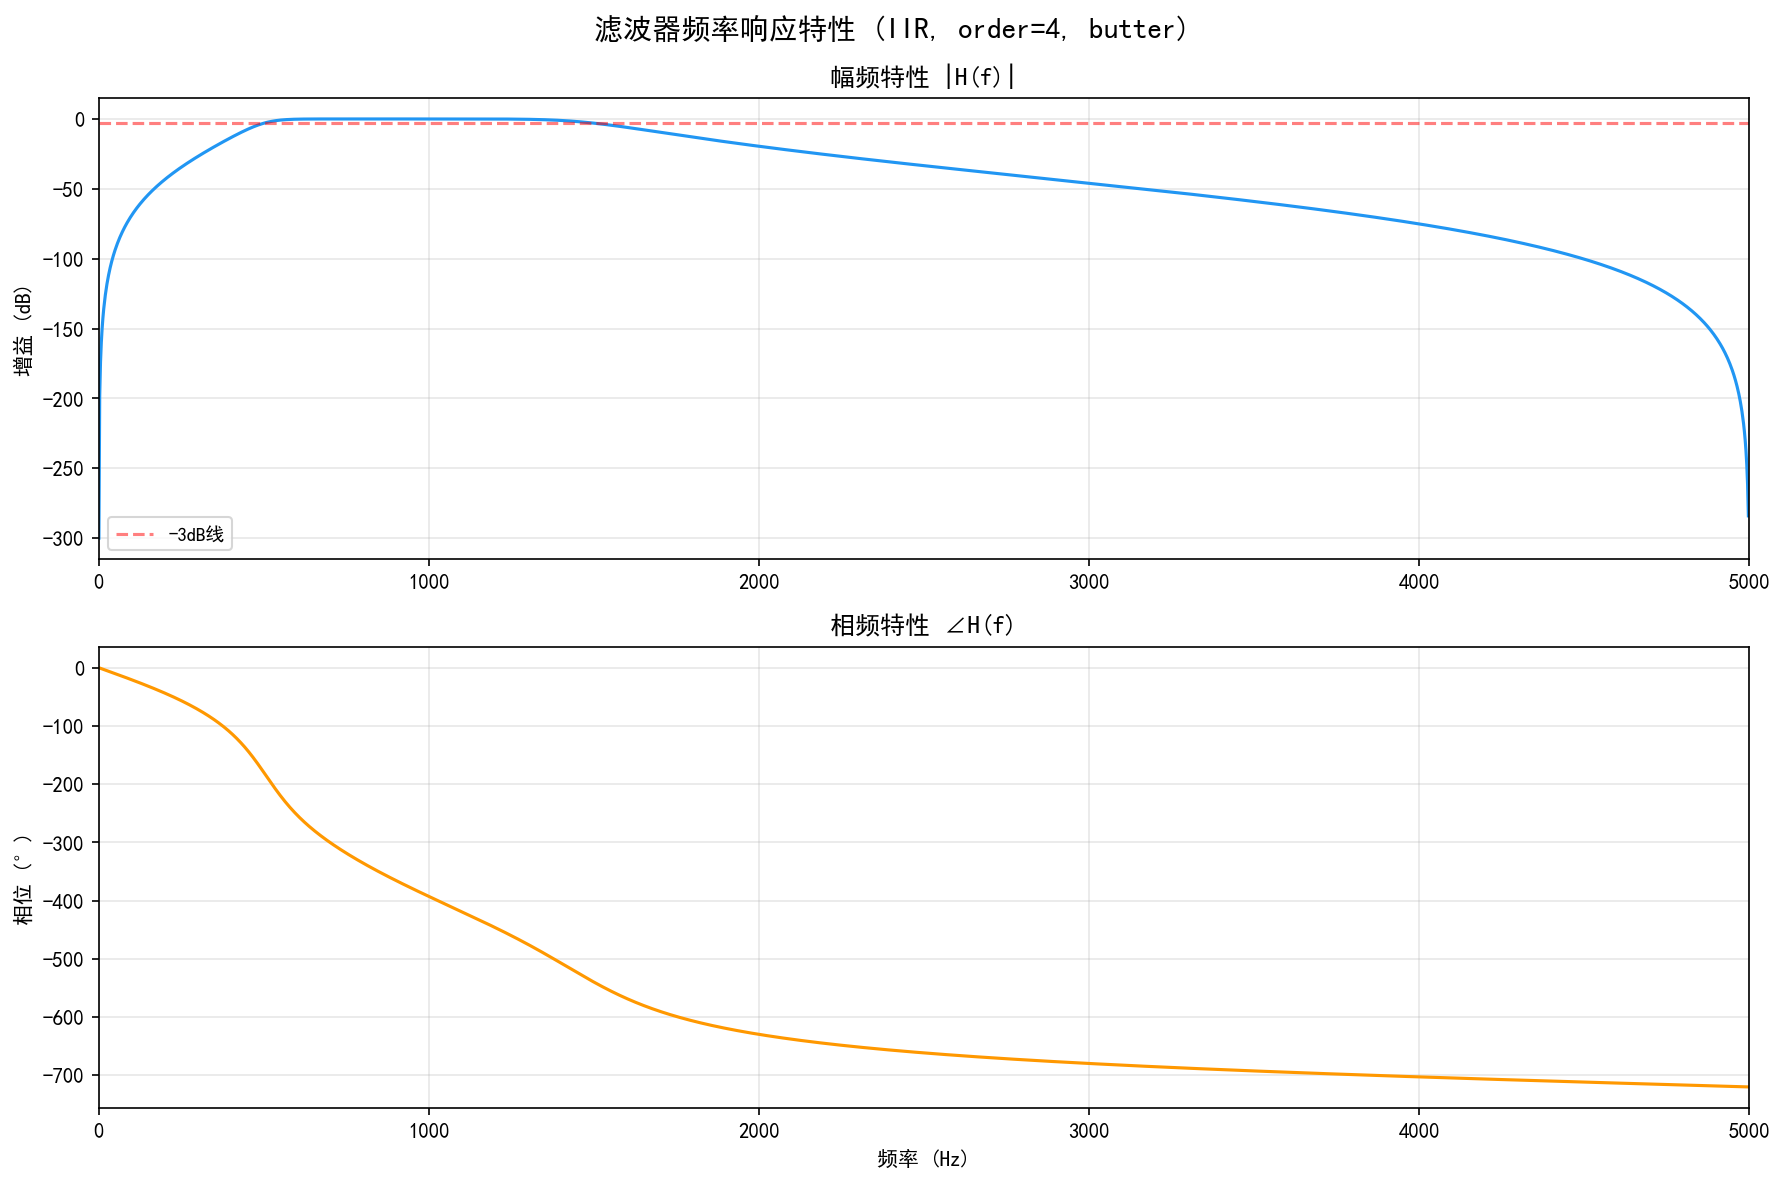
\includegraphics[width=\textwidth]{07_iir_response.png}
\end{minipage}
\caption{FIR（左，64 阶 Hamming）与 IIR（右，4 阶 Butterworth）带通滤波器幅频/相频特性}
\label{fig:firiir}
\end{figure}

三维参数扫描结果（图~\ref{fig:opt}）汇总于表~\ref{tab:best}：ASK/PSK 最优解均为 \textbf{FIR 32 阶 Kaiser}，FSK 最优为 \textbf{FIR 64 阶 Blackman}——FSK 需要分辨间隔 400\,Hz 的双峰，更高阶数带来的更窄过渡带收益大于计算代价；ASK/PSK 为单峰信号，32 阶 Kaiser（可调 $\beta$ 参数）在保真度与阻带衰减间取得最佳平衡。三种调制的最优带宽缩放均为 $\times 1.0$，表明名义带宽设计已接近最优，$\pm 20\%$ 偏离引起 $0.1\sim0.3$\,dB 的次级差异。IIR 全部组合均未胜出：其非线性相位虽被 filtfilt 消除，但同等阶数下阻带抑制弱于高阶 FIR。最优滤波器的幅频特性与 Z 域零极点形态见图~\ref{fig:best}（以 FSK 为例），零点均匀分布于阻带对应角度，极点位于通带边缘附近，符合带通选择性的零极点设计原理。

\begin{table}[H]
\centering
\caption{迭代优化最优滤波器组合（84 种组合/调制）}
\label{tab:best}
\begin{tabular}{ccccc}
\toprule
调制 & 最优组合 & 带宽缩放 & $\Delta$SNR (dB) & 保真度 \\
\midrule
ASK & FIR 32 阶 Kaiser & $\times 1.0$ & $+9.60$ & 0.9945 \\
FSK & FIR 64 阶 Blackman & $\times 1.0$ & $+8.10$ & 0.9924 \\
PSK & FIR 32 阶 Kaiser & $\times 1.0$ & $+9.27$ & 0.9940 \\
\bottomrule
\end{tabular}
\end{table}

\begin{figure}[htbp]
\centering
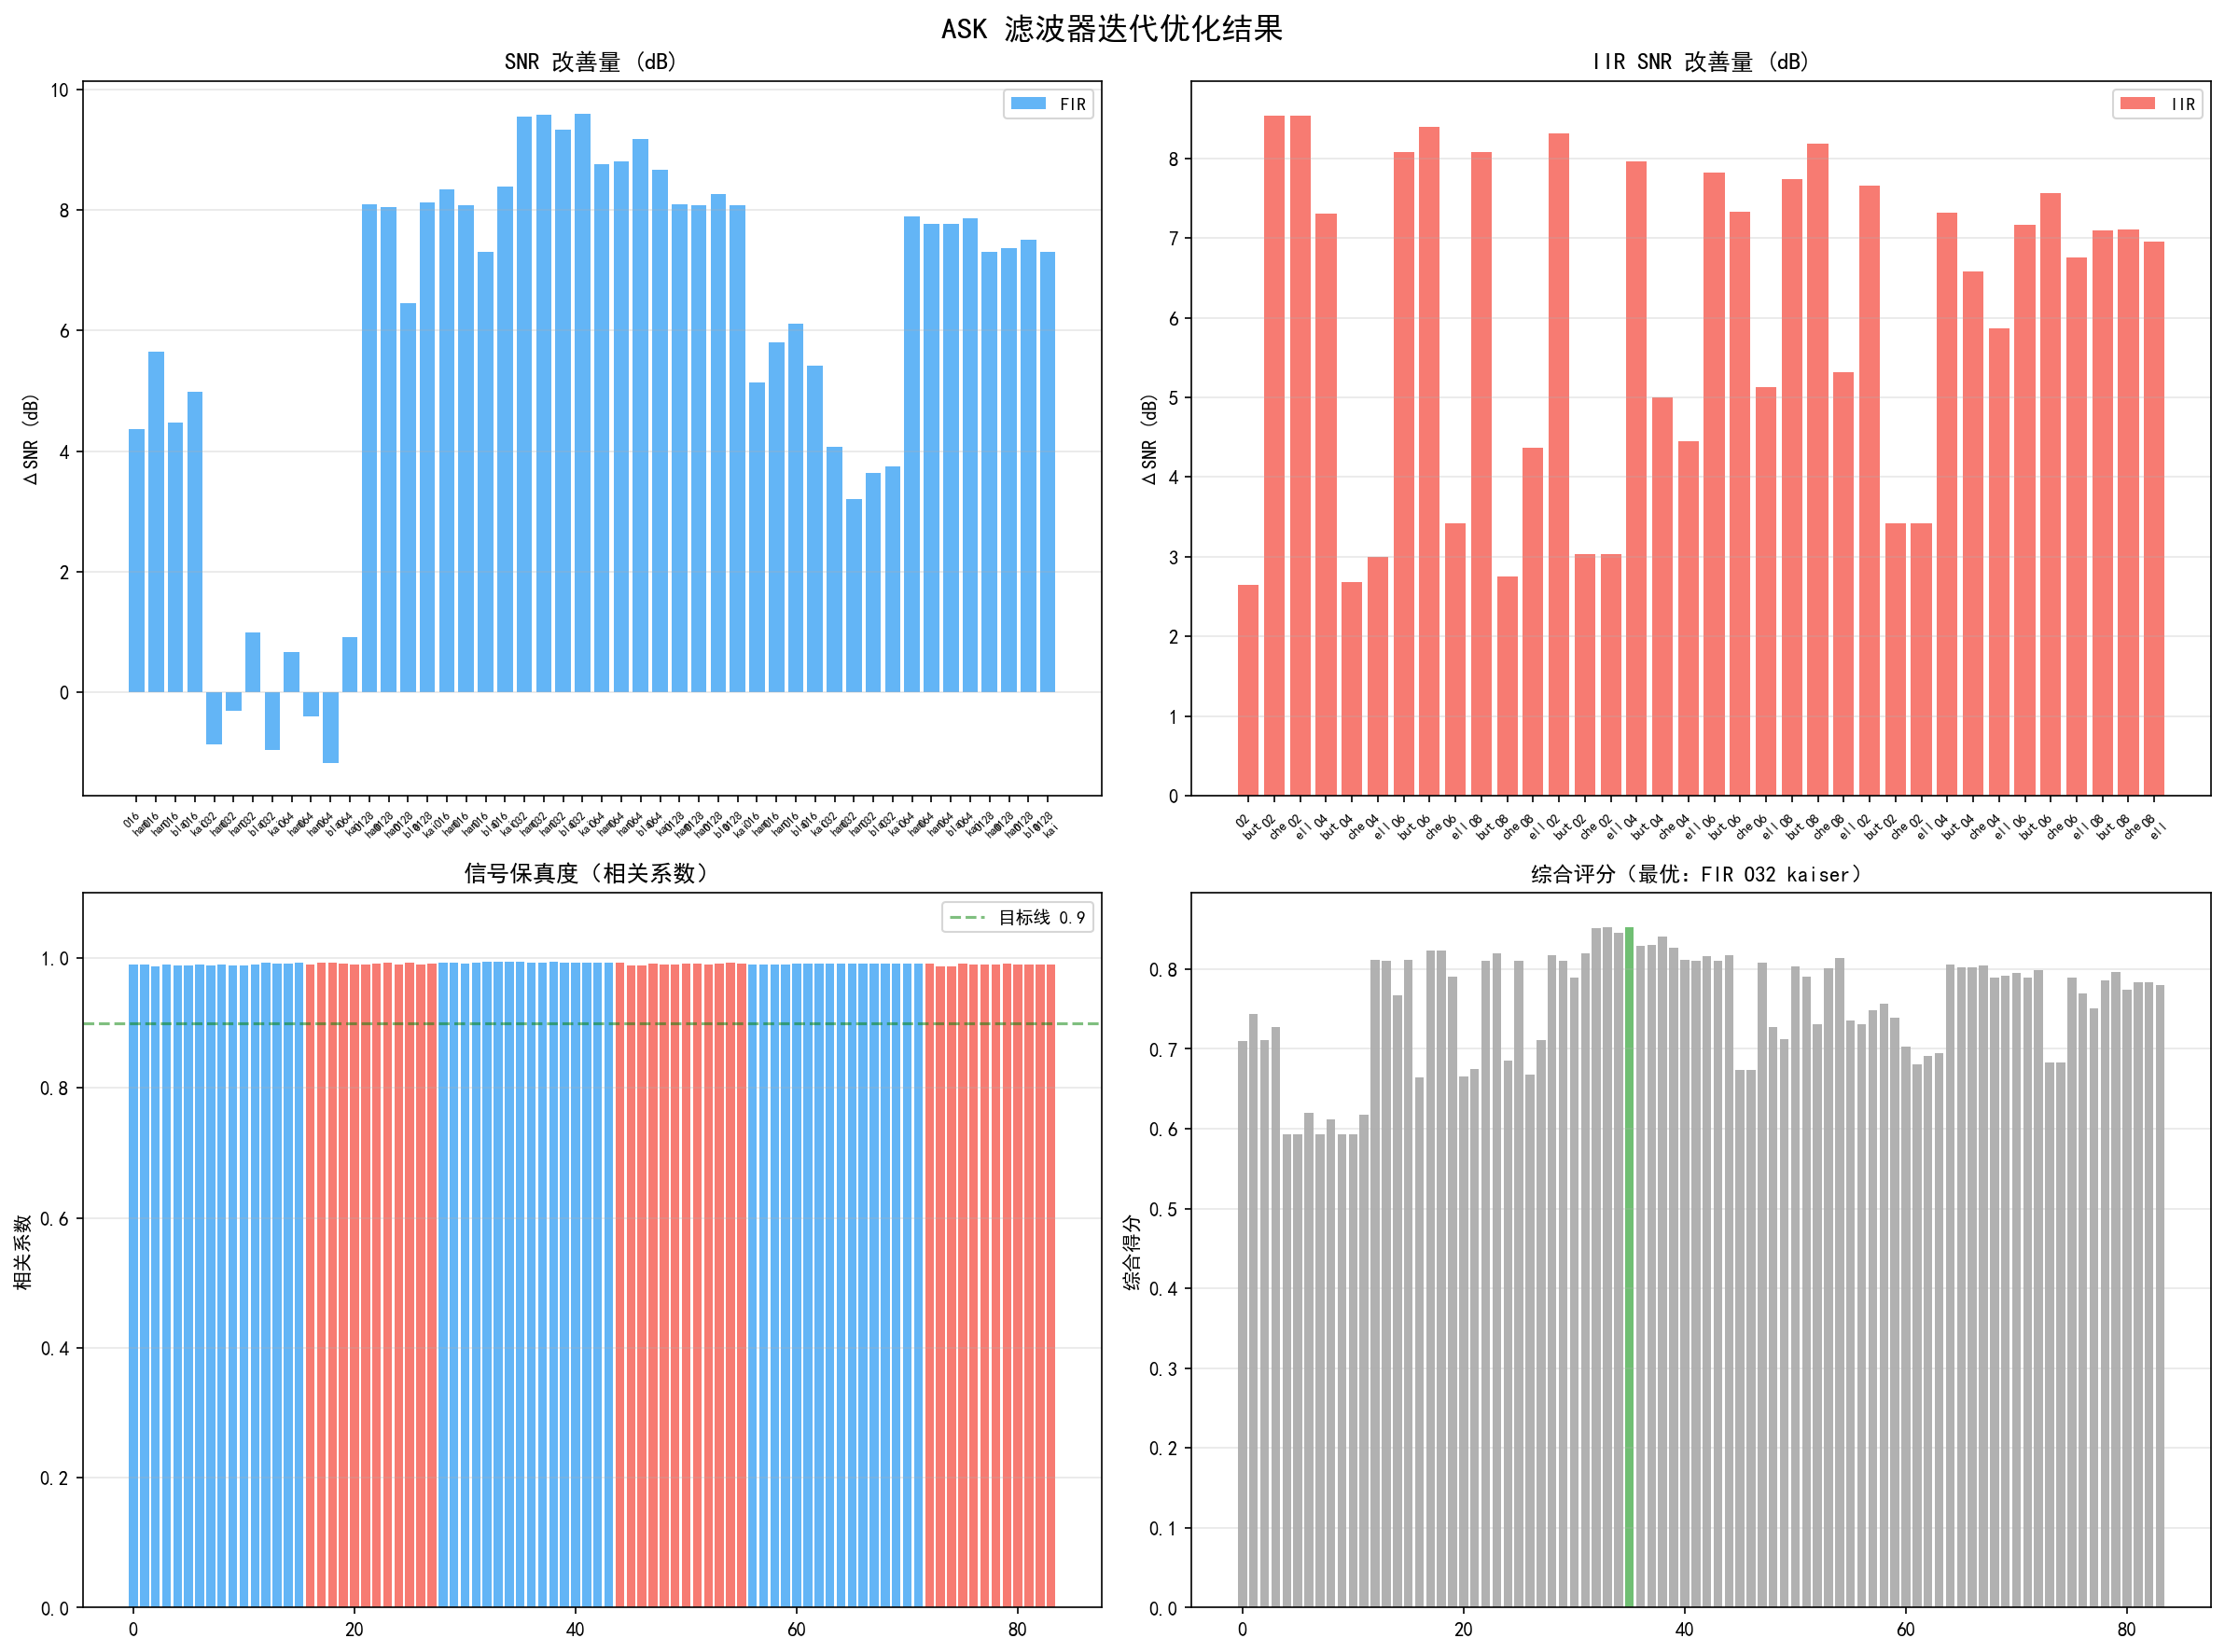
\includegraphics[width=0.85\textwidth]{09_ASK_optimization.png}
\caption{ASK 滤波器参数迭代优化（84 种组合扫描：SNR 改善/保真度/综合评分）}
\label{fig:opt}
\end{figure}

\begin{figure}[htbp]
\centering
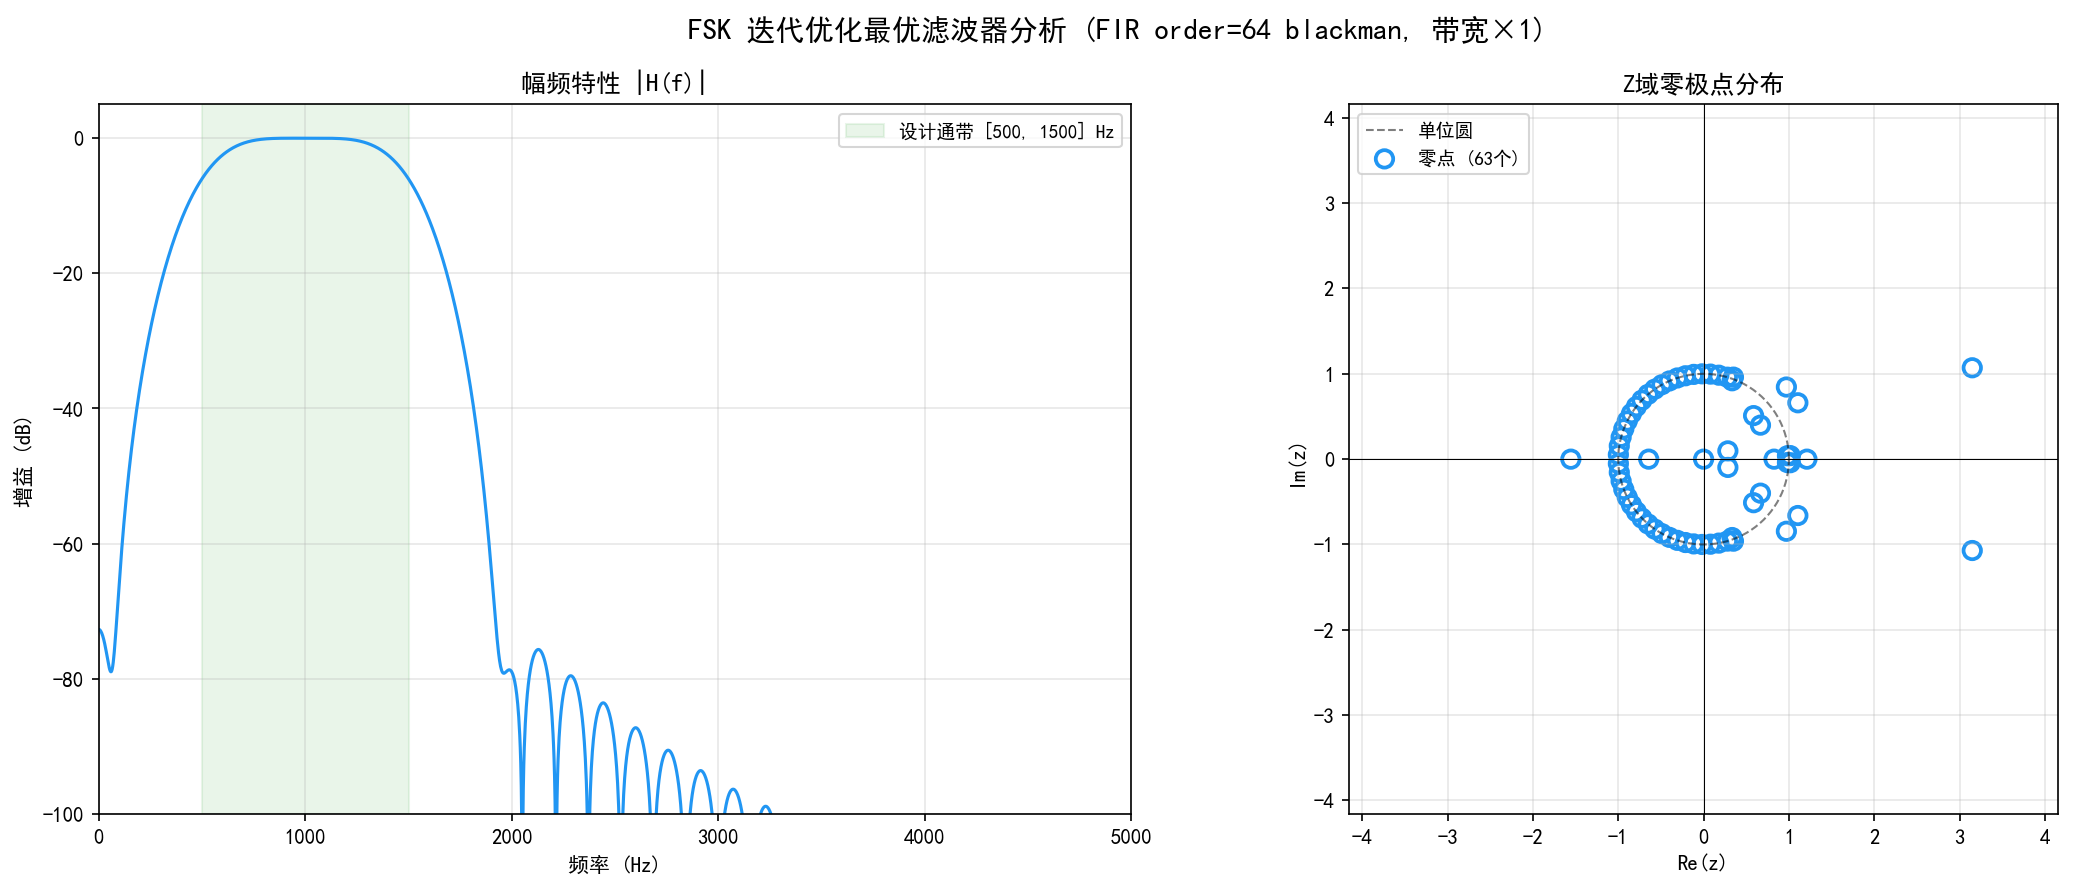
\includegraphics[width=0.98\textwidth]{09b_FSK_best_filter.png}
\caption{FSK 迭代优化最优滤波器分析（幅频特性+设计通带 / Z 域零极点分布）}
\label{fig:best}
\end{figure}

滤波前后波形对比（图~\ref{fig:filter}）显示 FIR 滤波有效抑制带外噪声，输出波形与纯净信号高度吻合。

\begin{figure}[htbp]
\centering
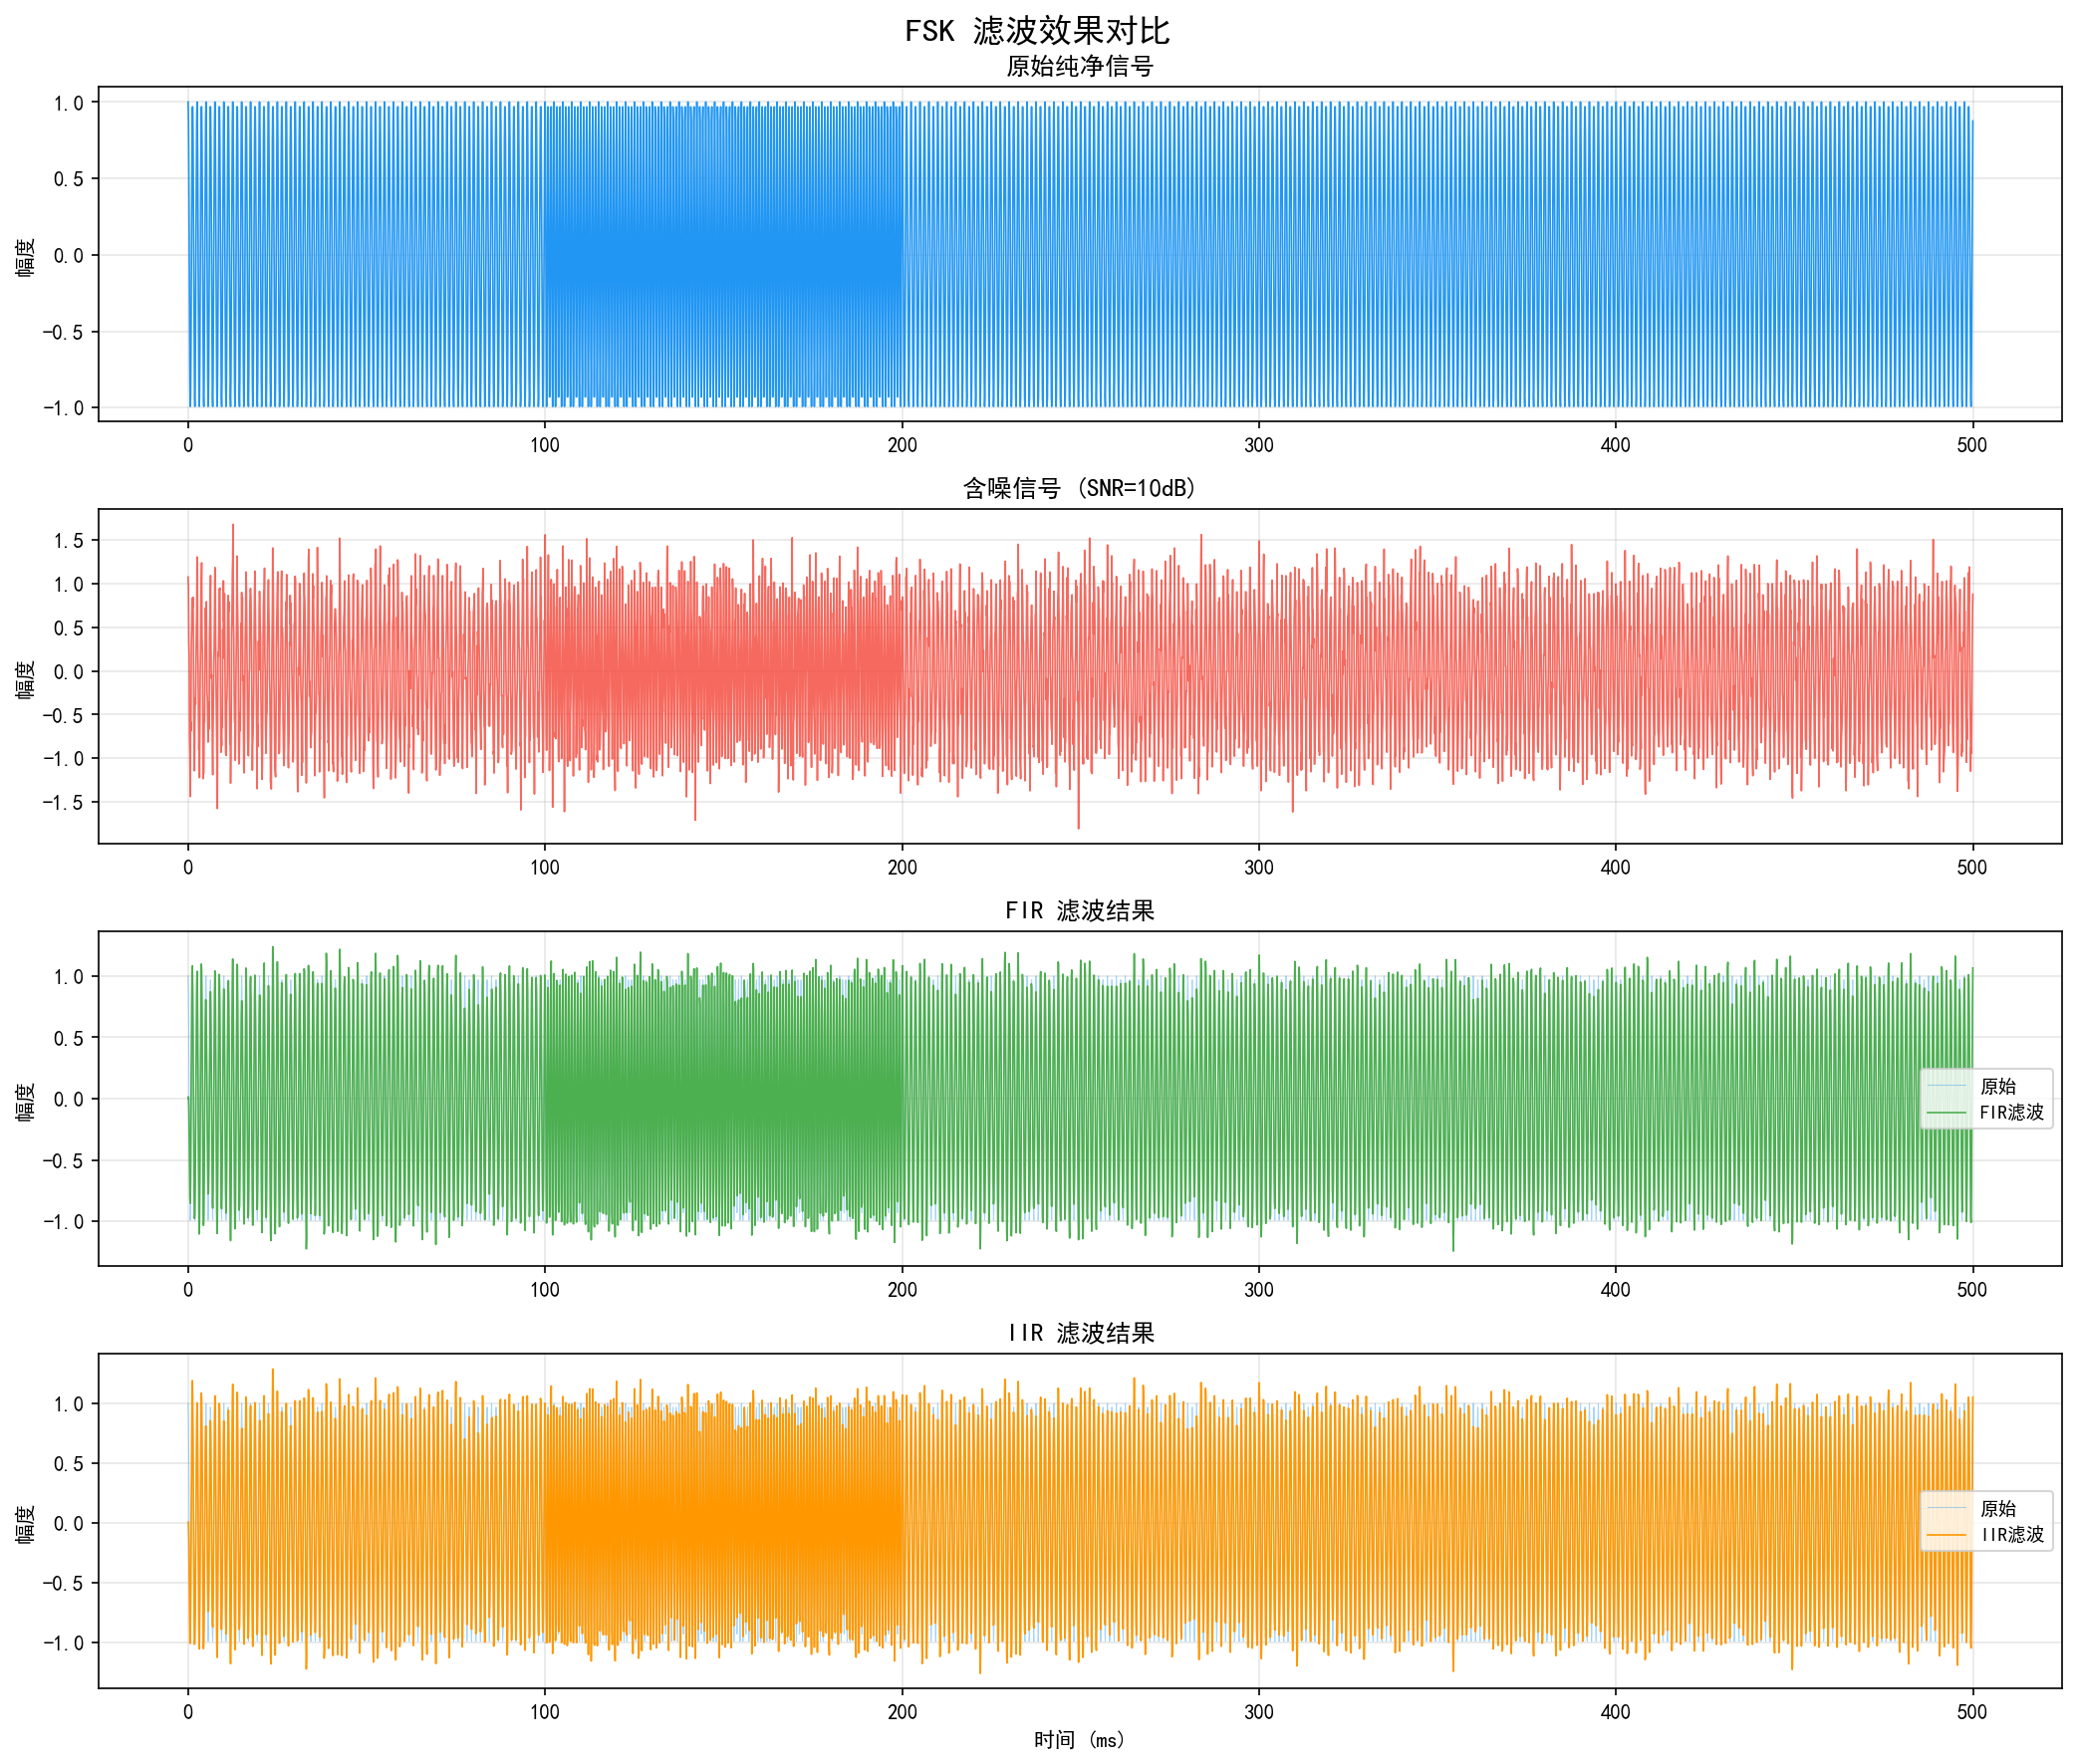
\includegraphics[width=0.75\textwidth]{08_FSK_filter_comparison.png}
\caption{FSK 滤波前后波形对比（纯净/含噪/FIR/IIR）}
\label{fig:filter}
\end{figure}

\subsection{NLMS 自适应滤波}

图~\ref{fig:lms} 为 ASK 的 NLMS 详细分析：MSE 收敛曲线（对数坐标）、不同步长性能对比、权值演化与学习曲线。权值 $w[0]$ 快速收敛到 1（其余趋于 0），与维纳解 $[1,0,\dots,0]$ 吻合，验证了 ANC 参考信道设计的正确性。表~\ref{tab:nlms} 的步长扫描呈现典型折中：$\mu=0.01$ 稳态最优（$\Delta$SNR $=+9.41$\,dB），$\mu\ge 0.5$ 因梯度噪声过大反而恶化。三种调制的最优步长均为 0.01，最终 NLMS 性能与 FIR 迭代最优相当（FSK 场景 NLMS $+9.02$\,dB 甚至优于 FIR 迭代最优的 $+8.10$\,dB）。

\begin{figure}[htbp]
\centering
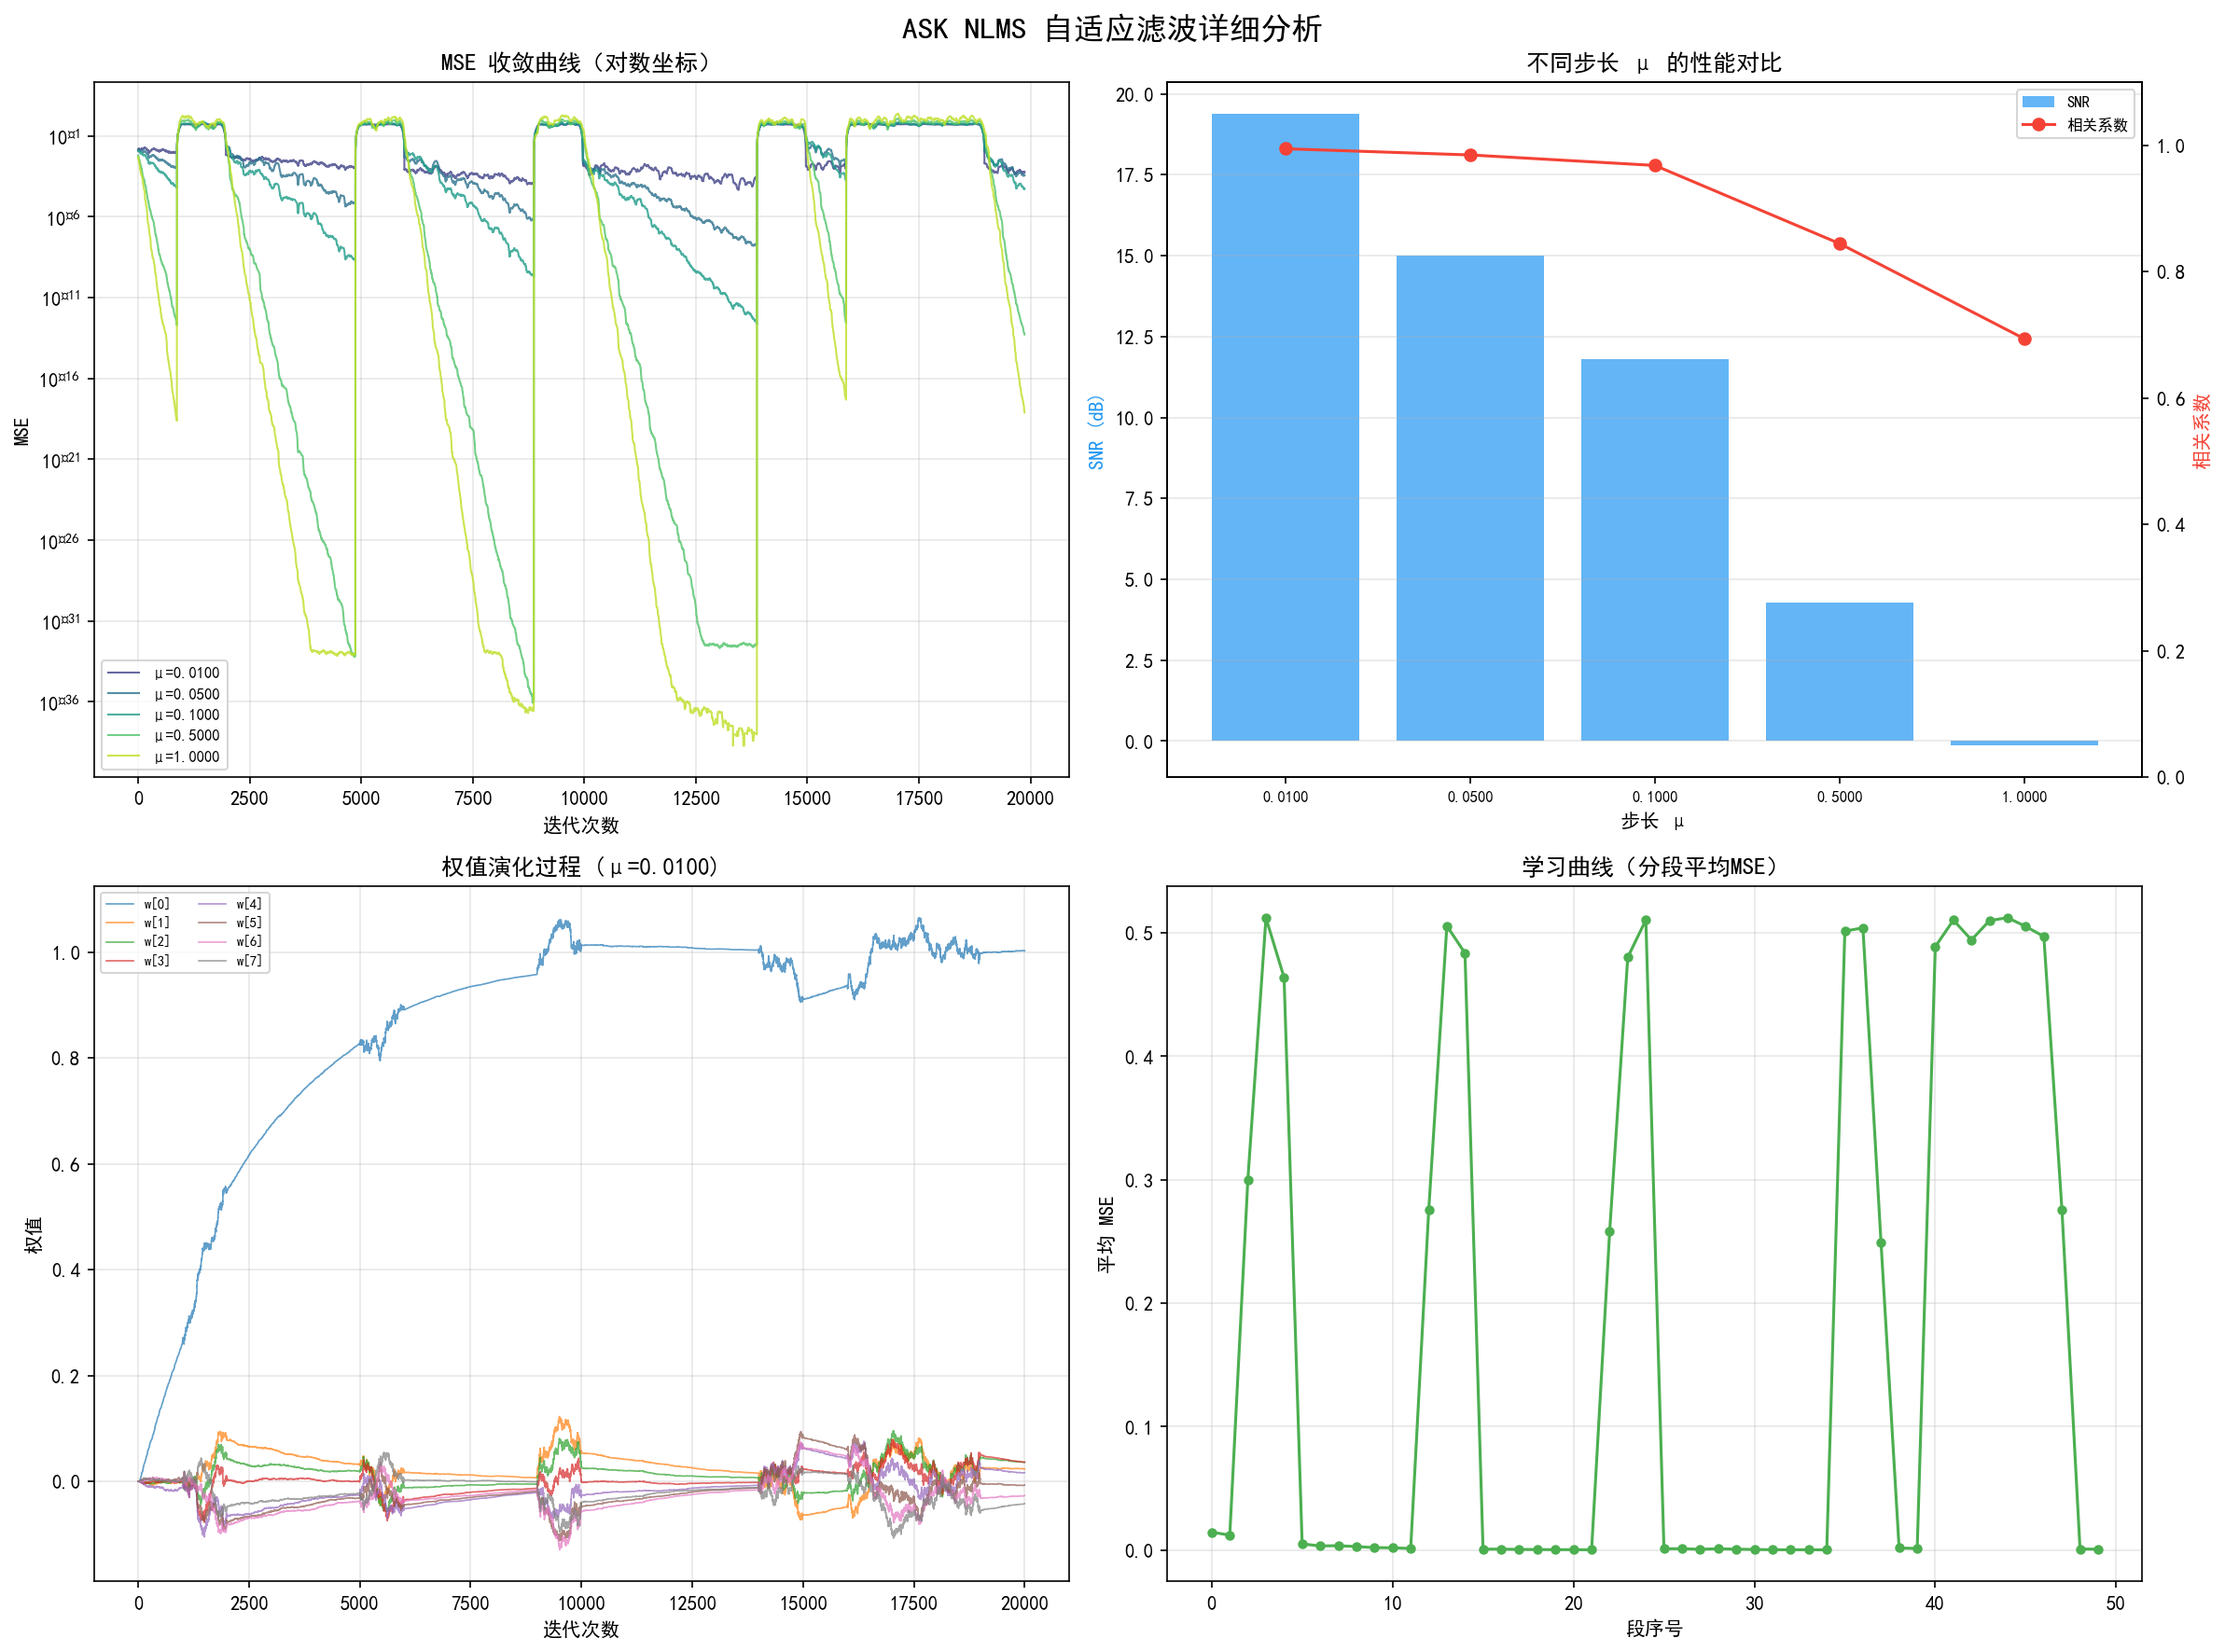
\includegraphics[width=0.88\textwidth]{10_ASK_lms_convergence.png}
\caption{ASK 的 NLMS 自适应滤波详细分析（收敛曲线/步长对比/权值演化/学习曲线）}
\label{fig:lms}
\end{figure}

\begin{table}[H]
\centering
\caption{NLMS 步长扫描结果（SNR=10\,dB）}
\label{tab:nlms}
\begin{tabular}{cccccc}
\toprule
调制 & $\mu$ & 输出 SNR (dB) & $\Delta$SNR (dB) & 相关系数 & 稳态 MSE \\
\midrule
ASK & 0.01 & 19.39 & $+9.41$ & 0.9943 & 0.2523 \\
ASK & 0.05 & 15.01 & $+5.03$ & 0.9845 & 0.2622 \\
ASK & 0.10 & 11.79 & $+1.81$ & 0.9679 & 0.2740 \\
ASK & 0.50 & 4.27 & $-5.71$ & 0.8443 & 0.3528 \\
FSK & 0.01 & 19.04 & $+9.02$ & 0.9938 & 0.4918 \\
PSK & 0.01 & 18.96 & $+9.00$ & 0.9937 & 0.5025 \\
\bottomrule
\end{tabular}
\end{table}

\begin{figure}[htbp]
\centering
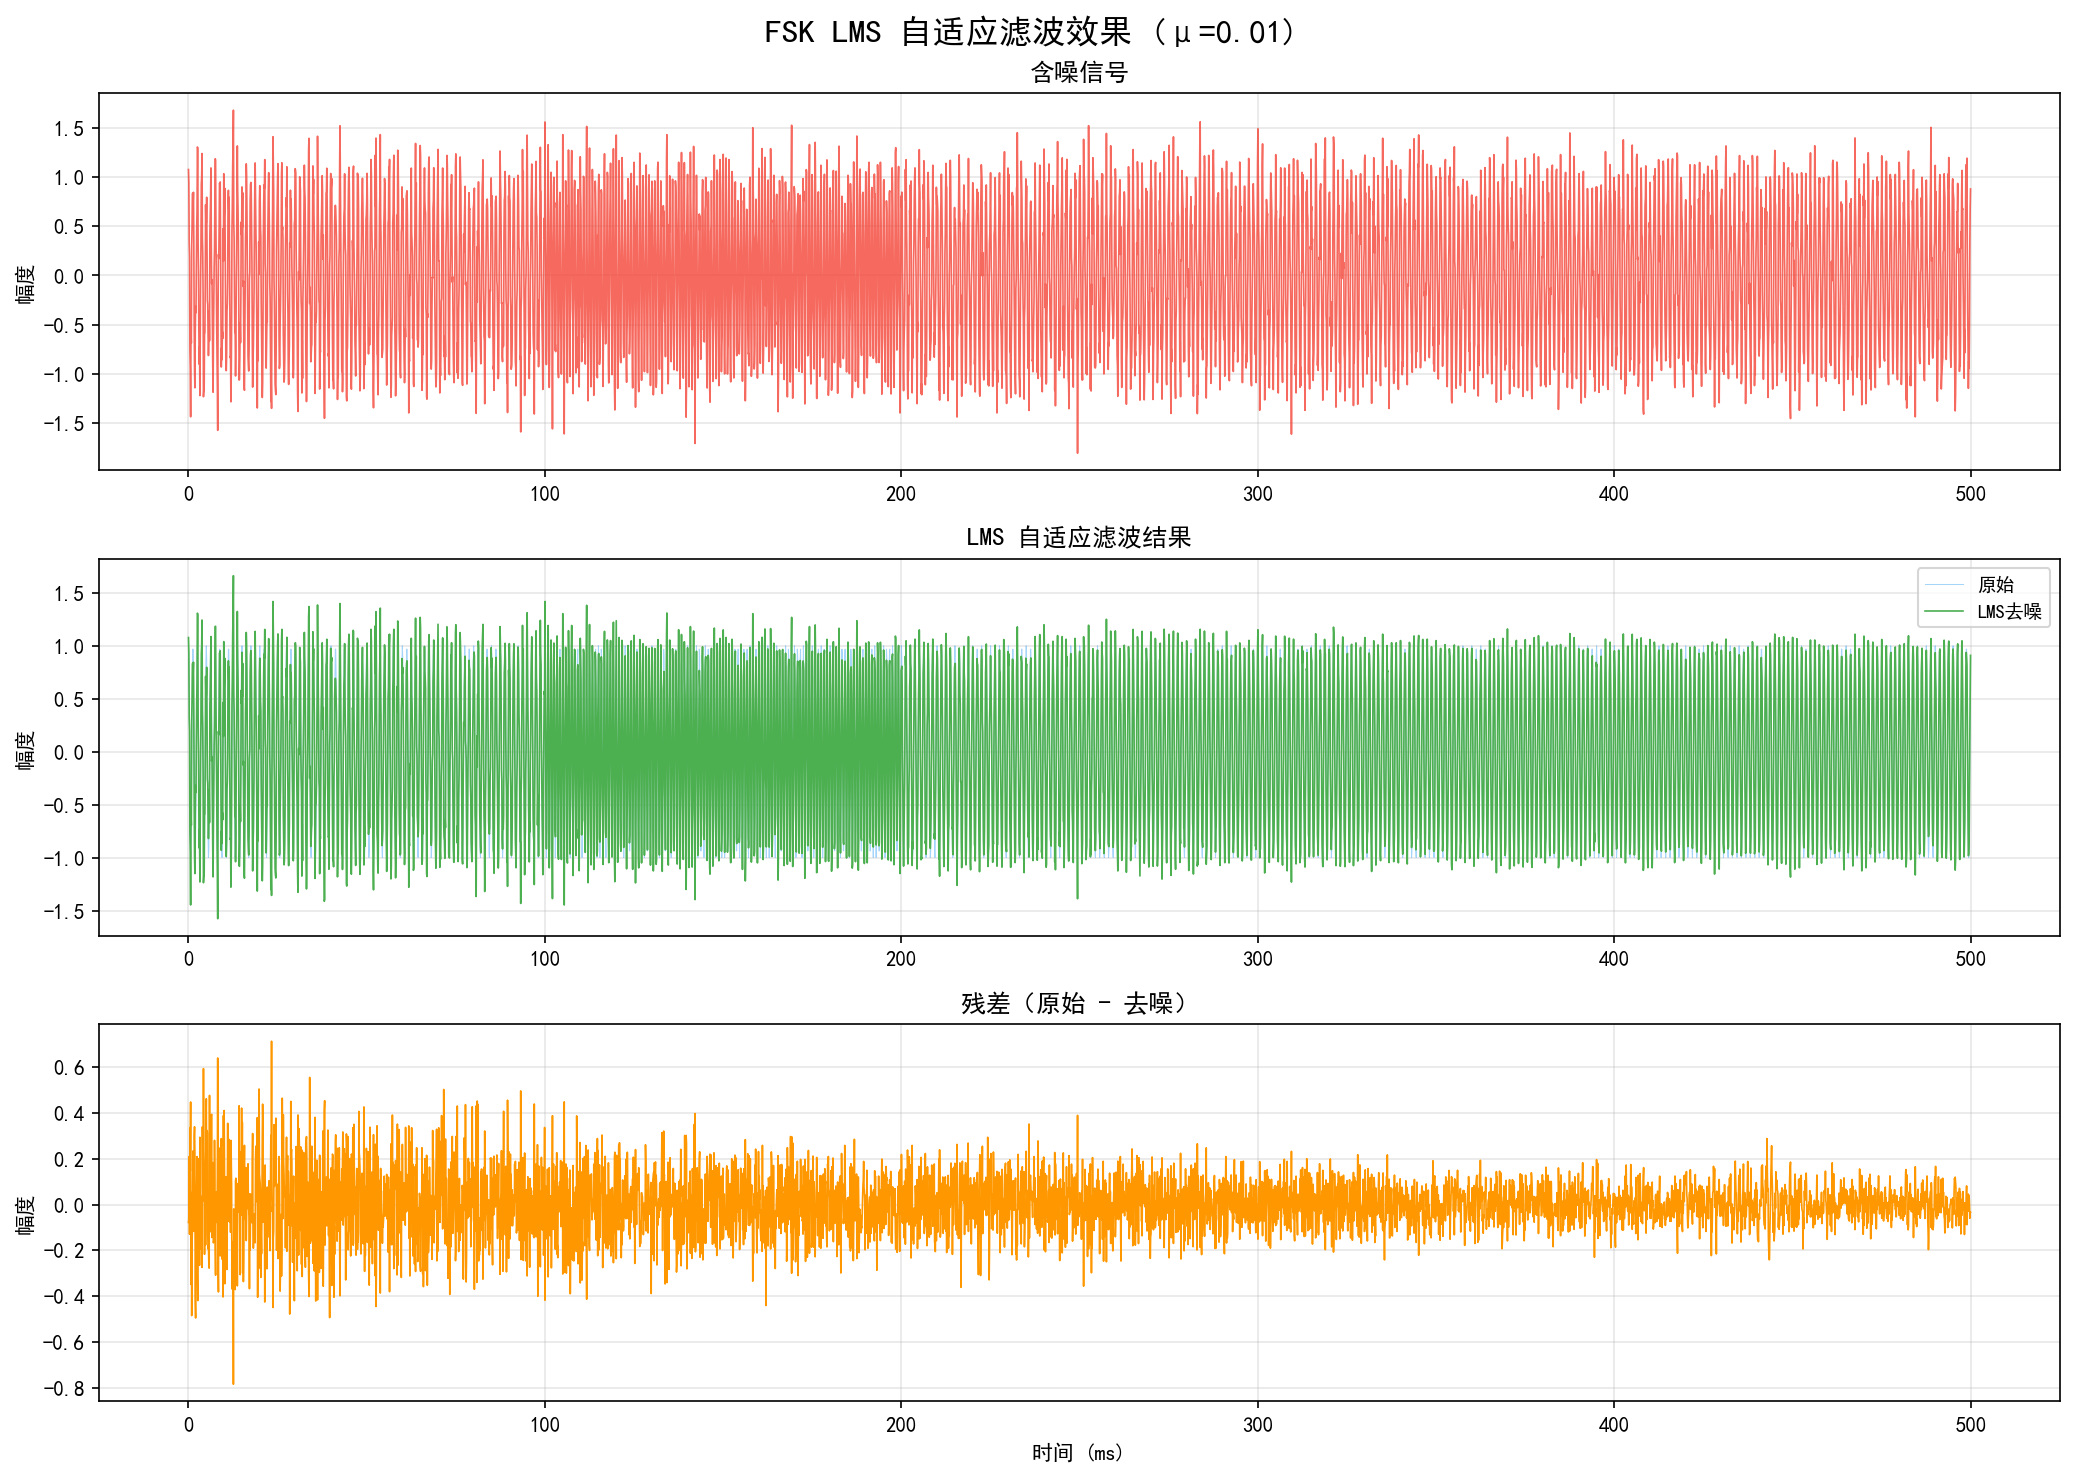
\includegraphics[width=0.78\textwidth]{10b_FSK_lms_waveform.png}
\caption{FSK 的 NLMS 去噪波形对比（含噪/去噪/残差）}
\label{fig:lmsw}
\end{figure}

\subsection{调制方式自动识别}

识别结果（图~\ref{fig:rec}）为 3/3 全部正确：ASK（置信度 73.7\%，依据：包络 CV=1.186、频谱单峰集中、Z 域谱线展宽 $r=0.956$）；FSK（52.2\%，双峰间隔 400\,Hz、Z 域尖锐谐振 $r=0.998$）；PSK（54.2\%，单峰恒包络窄带特征、$r=0.999$）。Z 域证据实际参与了每一例判决，体现多域联合设计。

\begin{figure}[htbp]
\centering
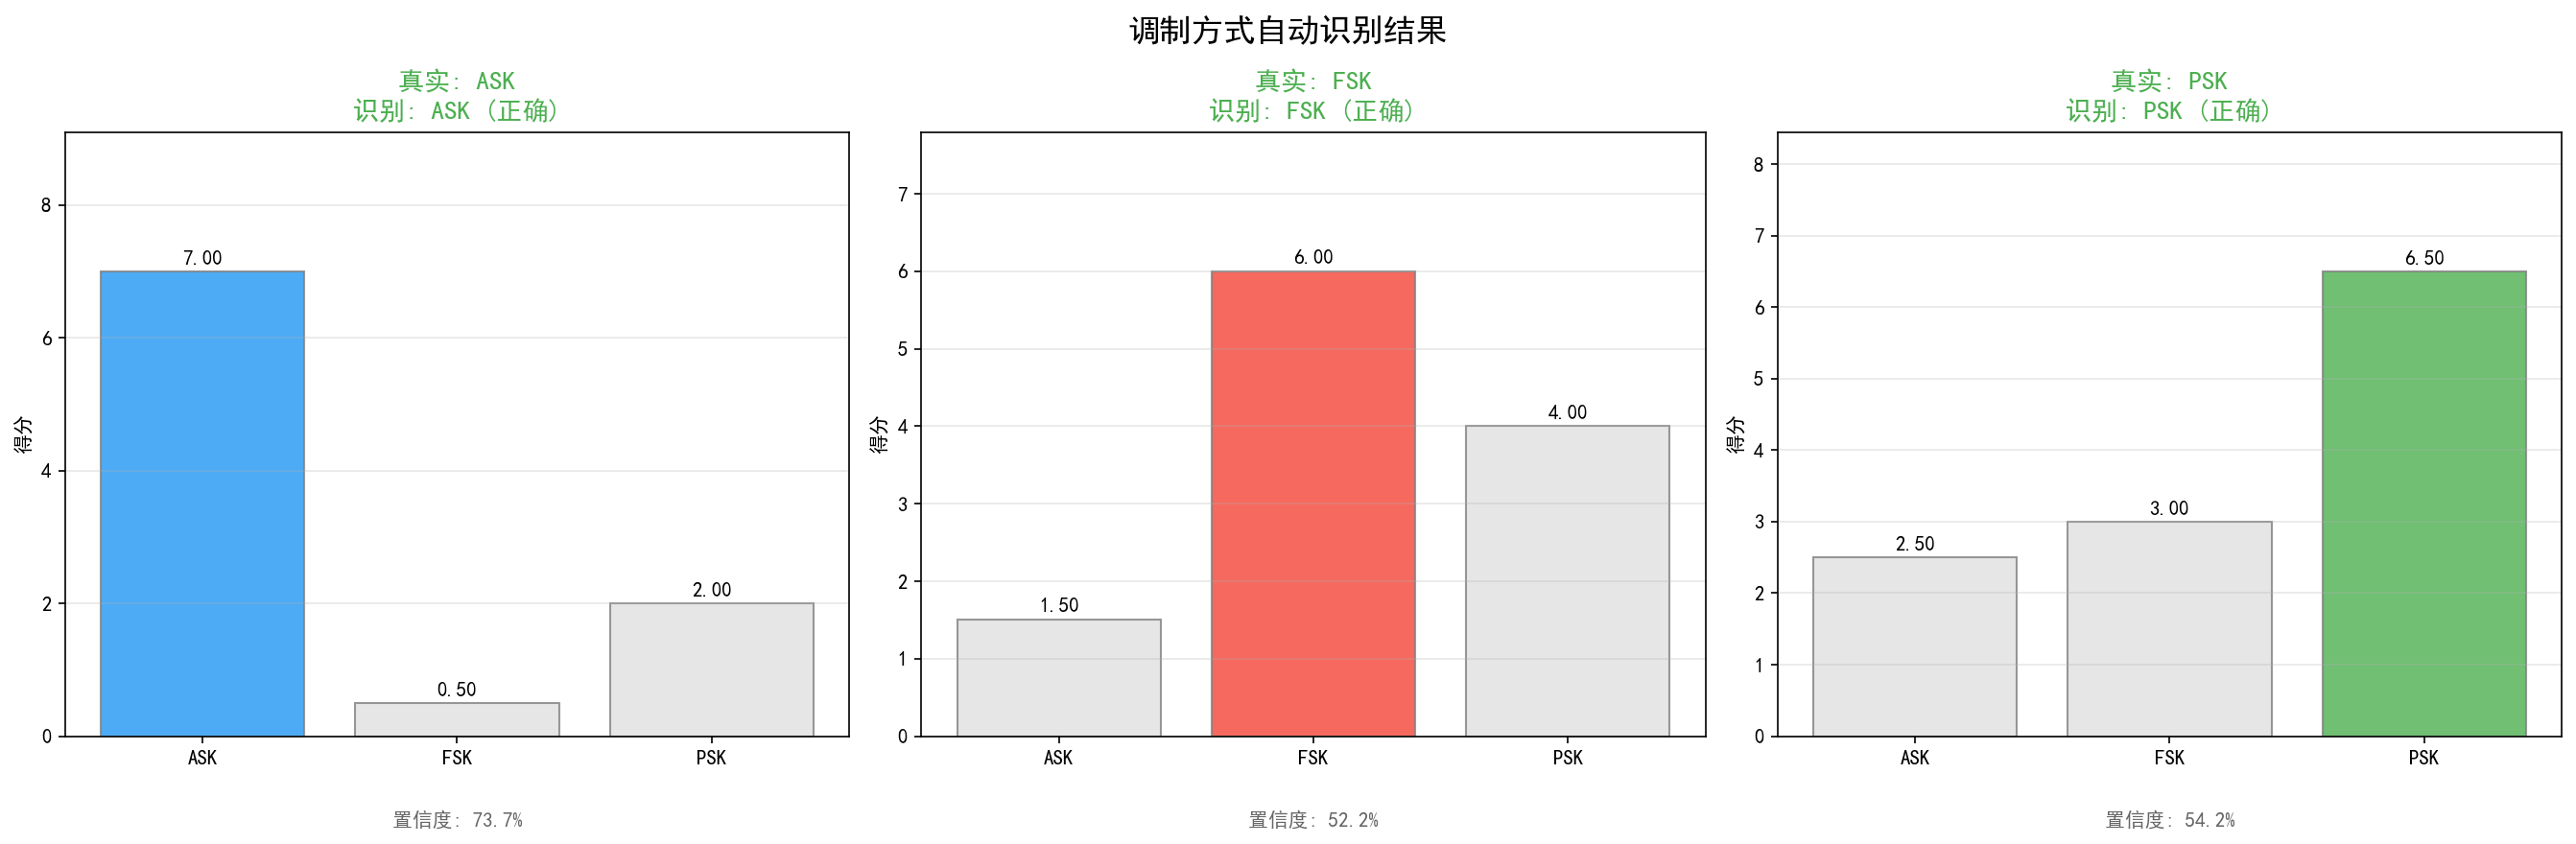
\includegraphics[width=0.98\textwidth]{11_recognition_result.png}
\caption{调制方式自动识别结果（SNR=10\,dB，准确率 100\%）}
\label{fig:rec}
\end{figure}

\subsection{综合性能评估：SNR、保真度、BER 与运算复杂度}

表~\ref{tab:perf} 汇总各滤波方法在 10\,dB 下的综合性能。要点：
\begin{enumerate}
  \item FIR 迭代最优取得最大 $\Delta$SNR（9.60\,dB）；NLMS 以 128 乘加/样本达到 9.41\,dB，接近 FIR；
  \item IIR 运算复杂度最低（34 乘加/样本，仅为 FIR 的 1/4），$\Delta$SNR 略低 1\,dB，适合资源受限场景；
  \item 所有滤波方法 BER 均为 0——10\,dB 下每符号 1000 点的相关解调处理增益极大，波形级差异在解调级被``消化''，这促使系统将 SNR 扫描扩展到深噪区间以暴露 BER 差异（见下节）。
\end{enumerate}

\begin{table}[H]
\centering
\caption{滤波方法综合性能评估（SNR=10\,dB，乘加/样本为 filtfilt 双向计）}
\label{tab:perf}
\begin{tabular}{lcccccc}
\toprule
调制 & 方法 & $\Delta$SNR (dB) & 保真度 & BER & 乘加/样本 & 耗时(ms) \\
\midrule
ASK & FIR 最优 & $+8.75$ & 0.9934 & 0 & 130 & 2.47 \\
ASK & IIR 最优 & $+7.96$ & 0.9921 & 0 & 34 & 0.00 \\
ASK & FIR 迭代最优 & $\bm{+9.60}$ & \textbf{0.9945} & 0 & 66 & 0.00 \\
ASK & NLMS 自适应 & $+9.41$ & 0.9943 & 0 & 128 & 151.6 \\
\midrule
FSK & FIR 最优 & $+7.95$ & 0.9921 & 0 & 130 & 2.00 \\
FSK & IIR 最优 & $+7.28$ & 0.9908 & 0 & 34 & 0.00 \\
FSK & FIR 迭代最优 & $+8.10$ & 0.9924 & 0 & 130 & 1.00 \\
FSK & NLMS 自适应 & $\bm{+9.02}$ & \textbf{0.9938} & 0 & 128 & 158.1 \\
\midrule
PSK & FIR 最优 & $+8.55$ & 0.9930 & 0 & 130 & 1.00 \\
PSK & IIR 最优 & $+7.83$ & 0.9917 & 0 & 34 & 0.95 \\
PSK & FIR 迭代最优 & $\bm{+9.27}$ & \textbf{0.9940} & 0 & 66 & 1.45 \\
PSK & NLMS 自适应 & $+9.00$ & 0.9937 & 0 & 128 & 158.3 \\
\bottomrule
\end{tabular}
\end{table}

\begin{figure}[htbp]
\centering
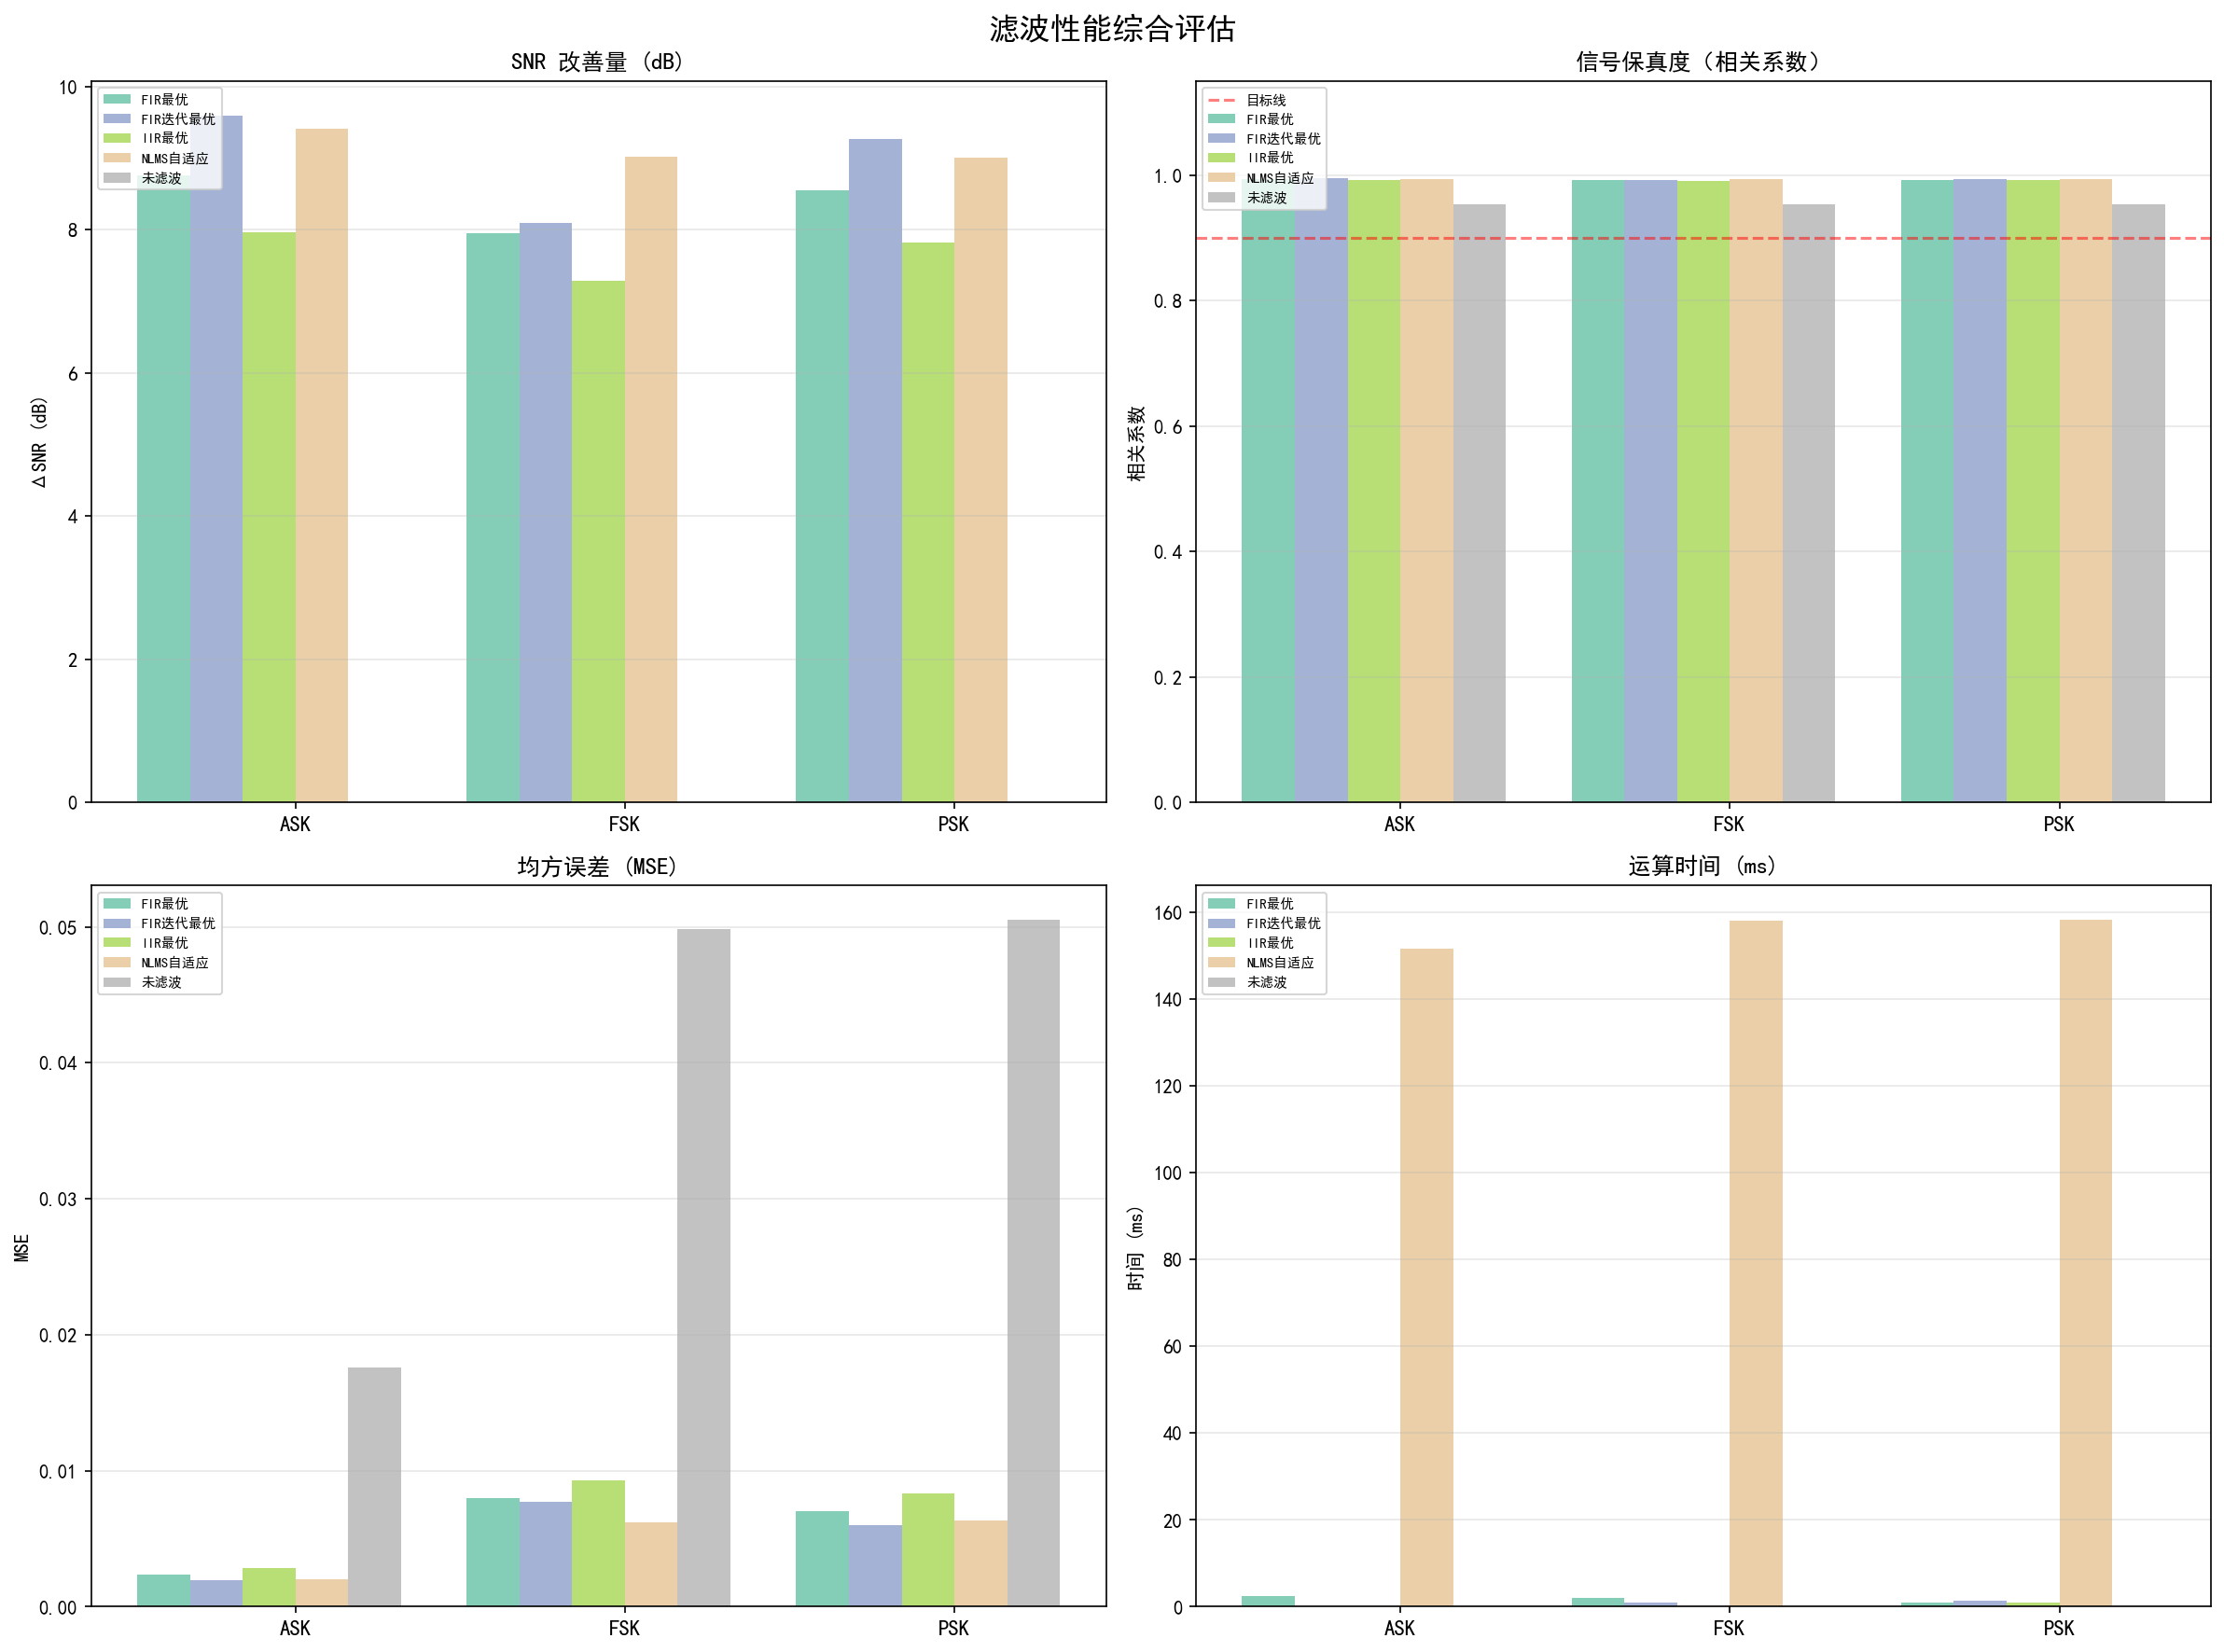
\includegraphics[width=0.88\textwidth]{12_performance_summary.png}
\caption{滤波性能综合评估（$\Delta$SNR/保真度/MSE/耗时）}
\label{fig:perf}
\end{figure}

\subsection{SNR 扫描蒙特卡洛实验}

表~\ref{tab:sweep} 与图~\ref{fig:sweep} 给出七个 SNR 点（每点 5 次独立试验）的平均性能。深噪区（$-25$\,dB）结果尤为关键：
\begin{itemize}
  \item \textbf{NLMS 展现压倒性优势}：$\Delta$SNR $=+23.24$\,dB（利用噪声参考直接对消），BER $=0.0067$，比 FIR（0.23）低 \textbf{34 倍}——在极低 SNR 下带外噪声已淹没带内，频率选择性滤波失效，而时域噪声对消仍然有效；
  \item \textbf{FIR 在中低 SNR（$-20\sim-15$\,dB）稳定优于未滤波}：BER 从 0.123 降至 0.077（$-20$\,dB）、0.093 降至 0.010（$-15$\,dB）；
  \item \textbf{识别准确率随 SNR 单调上升}：$-25$\,dB 时 27\%（接近随机），$-10$\,dB 起 93--100\%。
\end{itemize}

\begin{table}[H]
\centering
\caption{SNR 扫描蒙特卡洛结果（每点 5 次独立试验平均）}
\label{tab:sweep}
\begin{tabular}{cccccccc}
\toprule
SNR(dB) & $\Delta$SNR & $\Delta$SNR & $\Delta$SNR & BER & BER & BER & 识别 \\
 & FIR(dB) & IIR(dB) & NLMS(dB) & 未滤波 & FIR & NLMS & 准确率 \\
\midrule
$-25$ & 8.97 & 8.11 & 23.24 & 0.2000 & 0.2300 & \textbf{0.0067} & 27\% \\
$-20$ & 8.96 & 8.08 & 21.42 & 0.1233 & 0.0767 & 0.0100 & 40\% \\
$-15$ & 8.93 & 8.05 & 19.26 & 0.0933 & 0.0100 & 0.0067 & 67\% \\
$-10$ & 8.96 & 8.09 & 18.22 & 0 & 0 & 0.0033 & 93\% \\
0 & 8.94 & 8.08 & 13.62 & 0 & 0 & 0 & 100\% \\
10 & 8.47 & 7.72 & 9.00 & 0 & 0 & 0 & 100\% \\
20 & 5.53 & 5.30 & 2.96 & 0 & 0 & 0 & 100\% \\
\bottomrule
\end{tabular}
\end{table}

\begin{figure}[htbp]
\centering
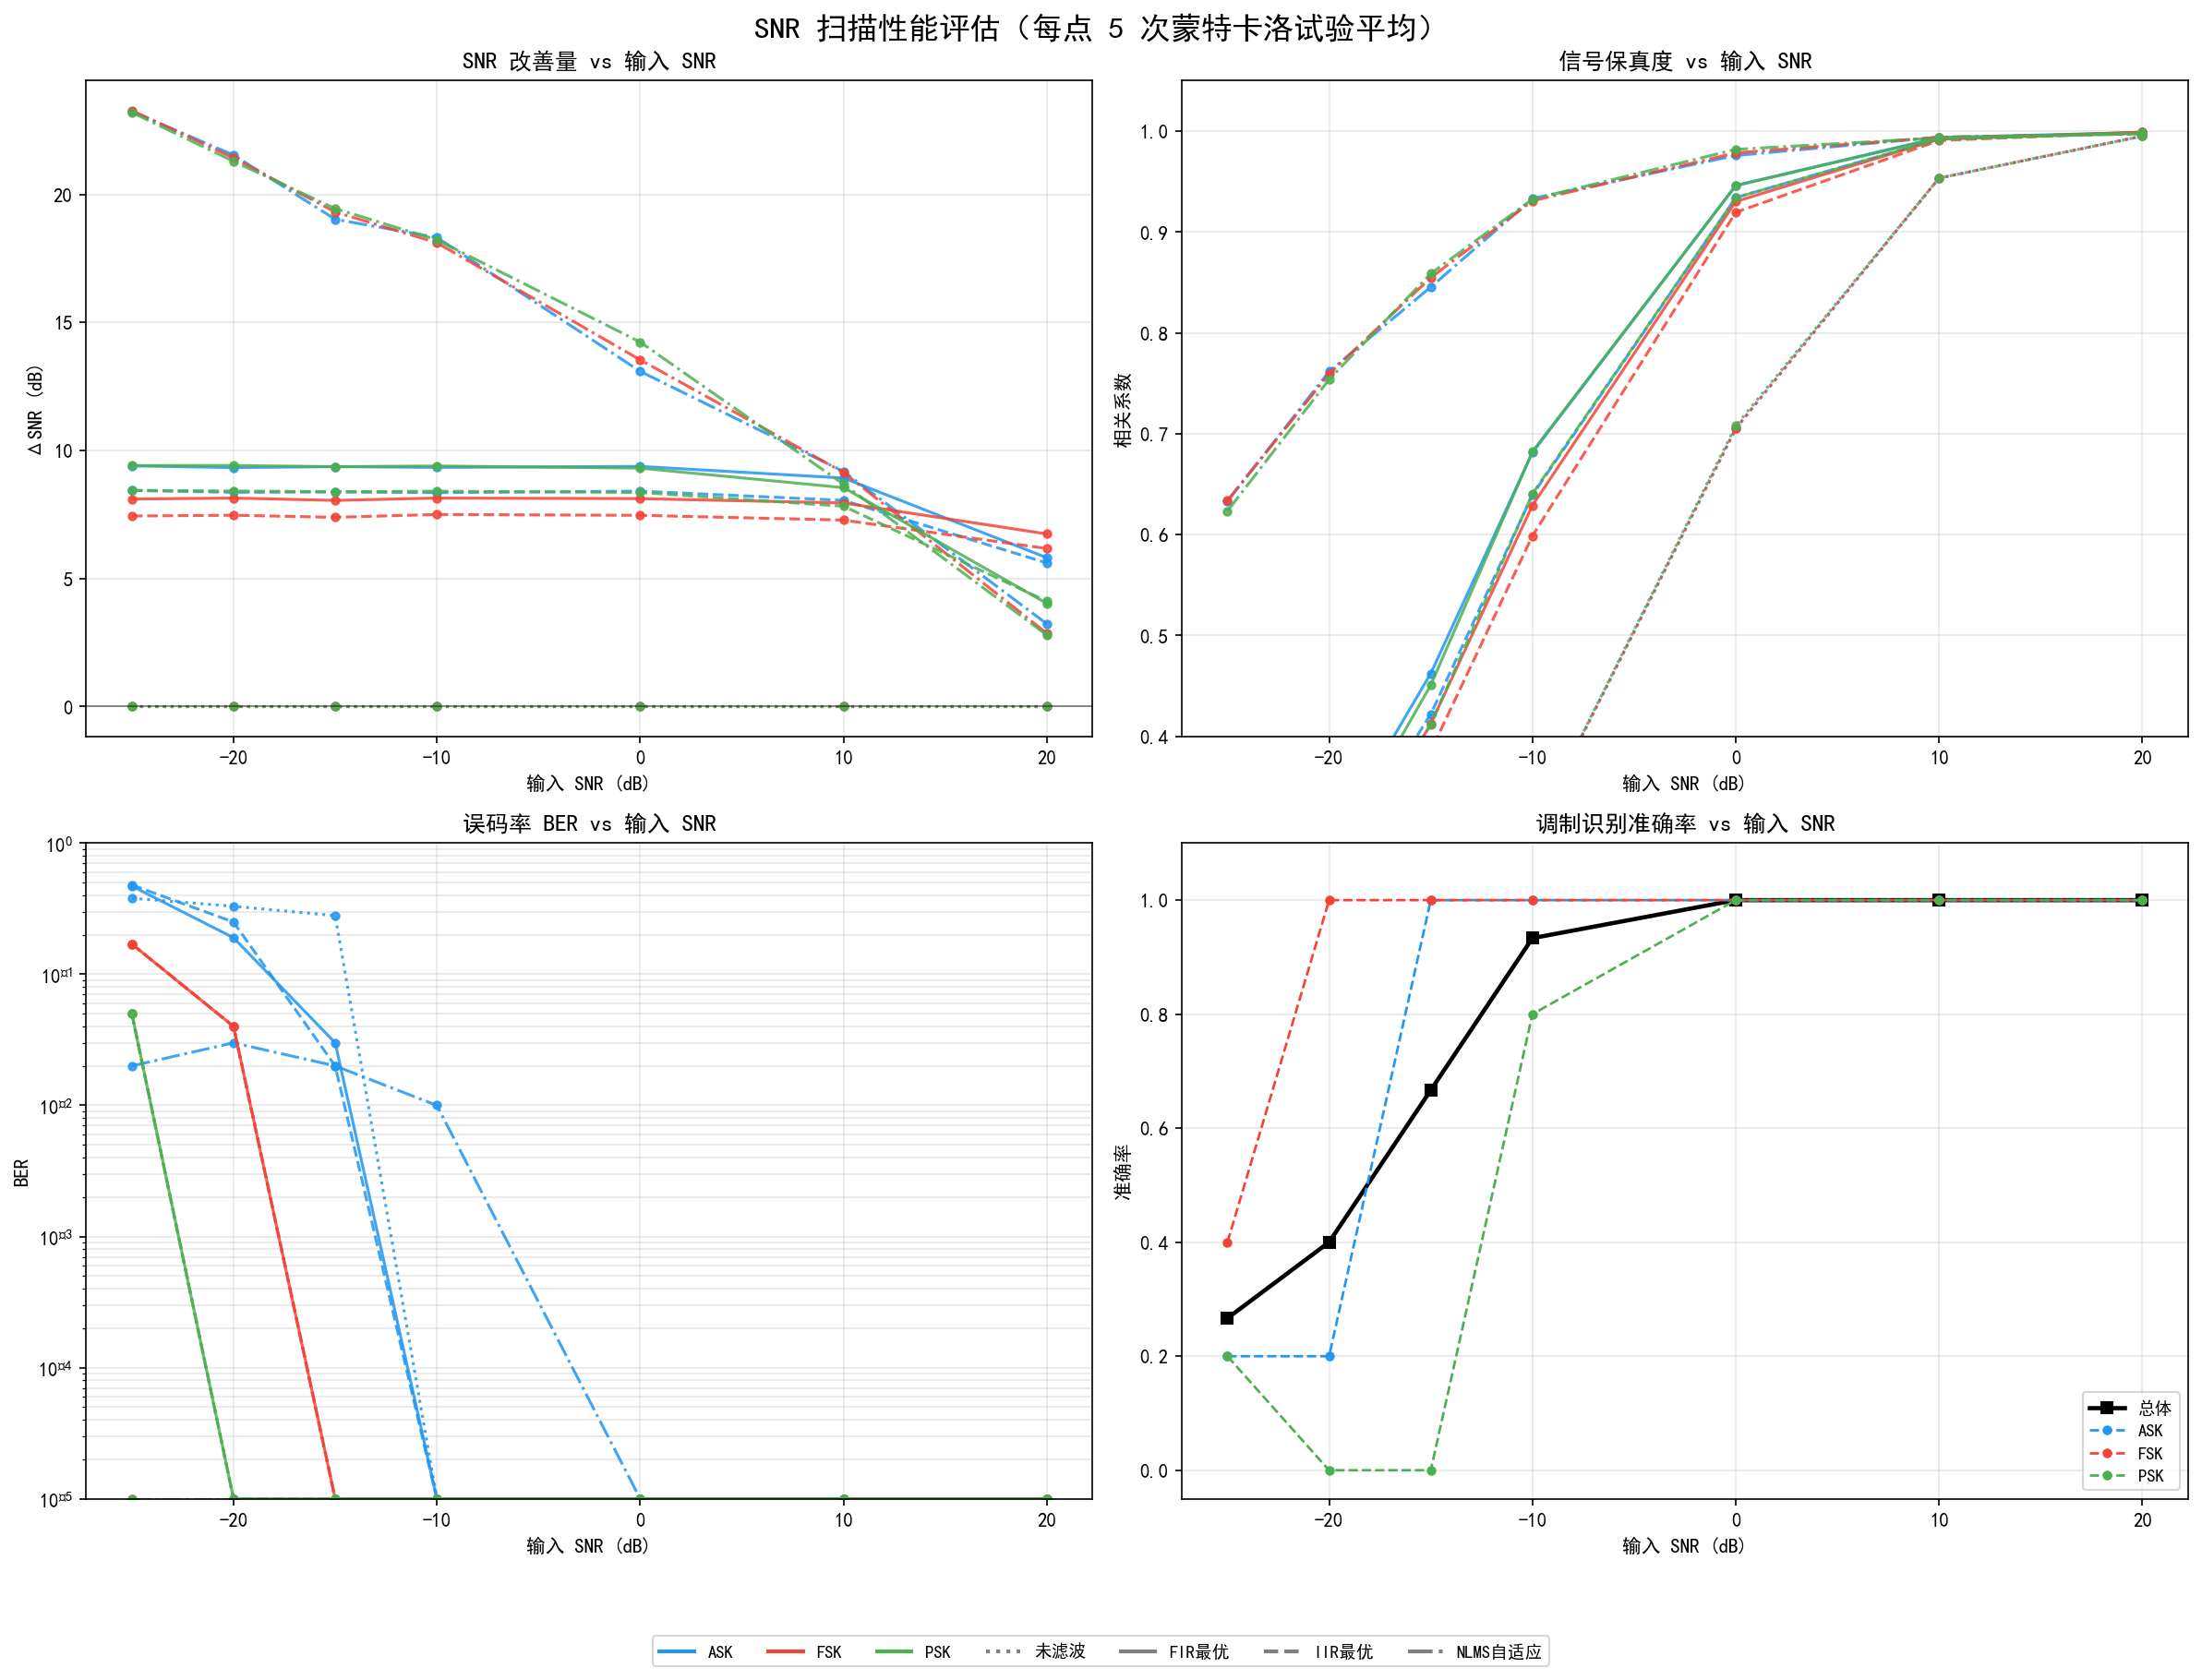
\includegraphics[width=0.85\textwidth]{14_snr_sweep.png}
\caption{SNR 扫描四联图（$\Delta$SNR/保真度/BER/识别准确率，颜色=调制方式，线型=滤波方法）}
\label{fig:sweep}
\end{figure}

\subsection{单一域 vs 多域联合消融实验}

表~\ref{tab:ablation} 为消融实验结果，直接回答题目``对比单一域处理与多域联合处理的优势''的要求：

\begin{table}[H]
\centering
\caption{单一域 vs 多域联合识别准确率消融（FIR 滤波后信号）}
\label{tab:ablation}
\begin{tabular}{ccccc}
\toprule
SNR(dB) & 仅时域 & 仅频域 & 仅Z域 & 多域联合 \\
\midrule
$-25$ & 33\% & 47\% & 33\% & 47\% \\
$-20$ & 33\% & 60\% & 47\% & \textbf{67\%} \\
$-15$ & 33\% & 67\% & 33\% & 47\% \\
$-10$ & 47\% & 67\% & 40\% & 53\% \\
0 & 67\% & 67\% & 53\% & \textbf{100\%} \\
10 & 67\% & 67\% & 40\% & \textbf{100\%} \\
20 & 67\% & 67\% & 47\% & \textbf{93\%} \\
\bottomrule
\end{tabular}
\end{table}

\textbf{核心发现}：
\begin{enumerate}
  \item \textbf{各单域均存在系统性盲区}：SNR$\ge 0$\,dB 时三个单域的准确率上限均为 67\%——时域无法区分 FSK/PSK（均恒包络）、频域无法区分 ASK/PSK（均单峰）、Z 域无法区分 FSK/PSK（均尖锐谐振），但三者盲区\textbf{互不重叠}；
  \item \textbf{多域联合消除盲区}：SNR$\ge 0$\,dB 平均准确率 97.8\%，相对最佳单域增益 $+31.1$ 个百分点；
  \item \textbf{深噪区融合无法创造信息}：SNR$<-10$\,dB 时各域特征本身失效，准确率共同退化——多域融合的前提是各域特征仍有效。
\end{enumerate}

\begin{figure}[htbp]
\centering
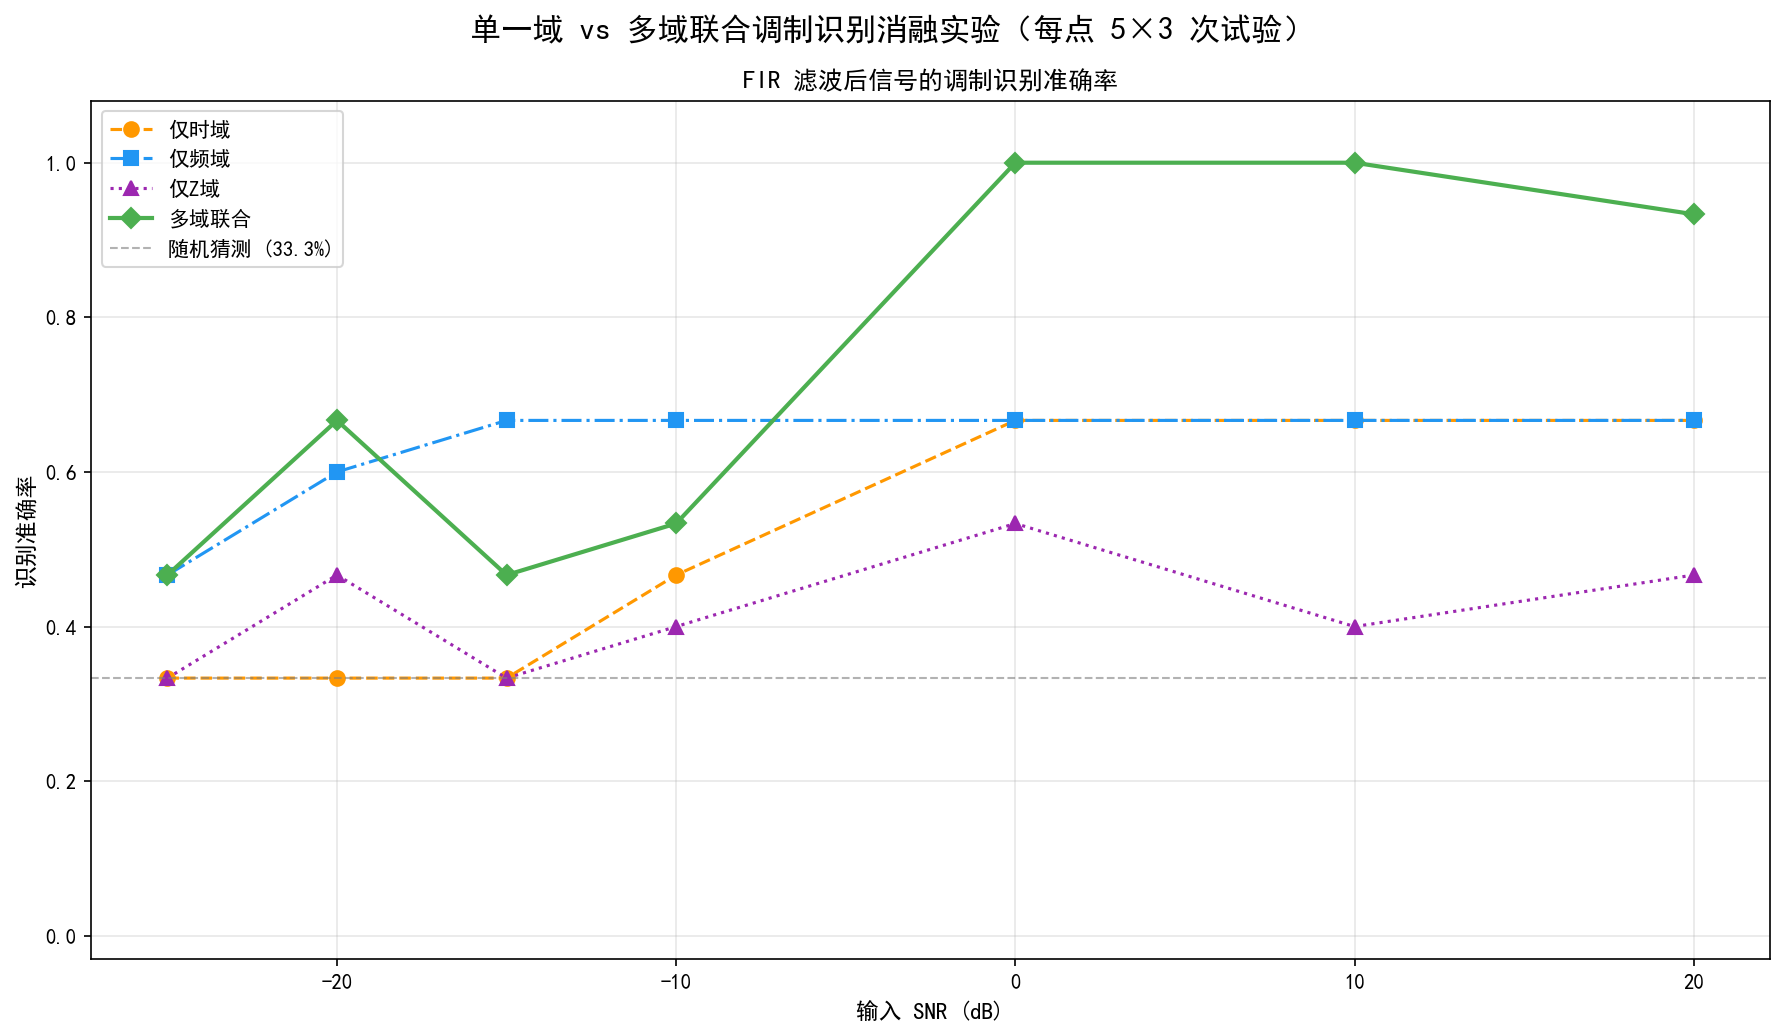
\includegraphics[width=0.75\textwidth]{16_domain_ablation.png}
\caption{单一域 vs 多域联合识别准确率消融曲线}
\label{fig:ablation}
\end{figure}

%==============================================================
\section{创新拓展与总结}
%==============================================================

\subsection{创新点}

\begin{enumerate}
  \item \textbf{NLMS 归一化自适应滤波}：在题目要求的``可自主尝试简单自适应滤波算法''基础上，针对标准 LMS 在白噪声参考下收敛慢的缺陷，实现步长与输入功率解耦的 NLMS，并通过候选步长按条件择优策略，使深噪区（$-25$\,dB）$\Delta$SNR 达 $+23.2$\,dB、BER 较 FIR 降低 34 倍；
  \item \textbf{解调级 BER 评估体系}：突破波形级指标局限，实现三种调制的完整解调链路（包络检波/相关/相干），揭示``滤波改善波形但 10\,dB 下 BER 均为零''的处理增益现象，并将扫描扩展至 $-25$\,dB 暴露方法间差异；
  \item \textbf{Z 域特征融入识别}：以 AR 主极点半径刻画谱线锐度，使``多域联合''名实相符；消融实验定量证明各单域盲区互补、多域增益 $+31.1\%$；
  \item \textbf{三维参数网格迭代优化}：阶数$\times$窗函数$\times$截止频率 84 组合/调制的自动扫描，以保真度与归一化 $\Delta$SNR 加权评分自动选型。
\end{enumerate}

\subsection{各变换工具的分工与协同}

\begin{itemize}
  \item \textbf{时域卷积}：低通平滑压制宽带噪声、提取包络/瞬时频率等调制特征，是识别的``第一道工序''；
  \item \textbf{DTFT}：连续谱形与带宽观察，指导带通滤波器截止频率设计；
  \item \textbf{DFT}：离散谱线与峰值检测，直接产出识别用的频域特征（双峰结构、谱集中度）；
  \item \textbf{Z 变换}：零极点将``谱线锐度''映射为极点半径这一系统级特征，并支撑滤波器零极点形态分析；
  \item \textbf{滤波器}：FIR 线性相位保形、IIR 低复杂度高效、NLMS 时域对消，三者按场景互补。
\end{itemize}

\subsection{局限与展望}

（1）识别规则阈值与当前参数（$F_s$、符号率、频点间隔）耦合，迁移到其他参数体制需重新标定；（2）NLMS 依赖理想噪声参考，实际系统中参考信道噪声与信道噪声仅部分相关，可进一步研究延迟参考 ANC 与自适应谱线增强器（ALE）；（3）深噪区识别准确率仍低，可引入高阶累积量或深度学习分类器；（4）蒙特卡洛试验次数可进一步增大以收窄 BER 置信区间。

%==============================================================
\appendix
\section{附录：关键程序代码}

以下代码直接引自工程源文件，与提交的运行结果一一对应。完整工程含 7 个源文件约 3600 行，此处收录核心实现。

\subsection{全局参数配置（config.py，节选）}
\lstinputlisting[linerange={10-72}]{config.py}

\subsection{信号生成（utils/generator.py）}
\lstinputlisting[linerange={14-208}]{utils/generator.py}

\subsection{多域分析核心算法（utils/analyzer.py，节选）}
时域特征与卷积平滑：
\lstinputlisting[linerange={19-79}]{utils/analyzer.py}
DFT/DTFT/Z 域零极点：
\lstinputlisting[linerange={84-241}]{utils/analyzer.py}

\subsection{滤波器设计与自适应滤波（utils/filter\_design.py，节选）}
FIR/IIR 设计与零相位滤波：
\lstinputlisting[linerange={19-136}]{utils/filter_design.py}
迭代优化主循环：
\lstinputlisting[linerange={248-374}]{utils/filter_design.py}
LMS/NLMS 自适应滤波：
\lstinputlisting[linerange={563-675}]{utils/filter_design.py}

\subsection{解调与误码率（utils/demodulator.py）}
\lstinputlisting[linerange={16-175}]{utils/demodulator.py}

\subsection{特征提取与调制识别（utils/recognizer.py，节选）}
Z 域特征与时频特征提取：
\lstinputlisting[linerange={21-195}]{utils/recognizer.py}
加权投票分类器（支持单域/多域模式）：
\lstinputlisting[linerange={197-326}]{utils/recognizer.py}
单域 vs 多域消融实验：
\lstinputlisting[linerange={786-839}]{utils/recognizer.py}

\subsection{主流程（main.py）}
\lstinputlisting[linerange={44-516}]{main.py}

\end{document}
